\chapter{Evaluation}

\section{Representative Benchmarks}
To determine the advantage provided by the core concept of the project requires assessing the impact of:
\begin{enumerate}
    \setlength\itemsep{0em}
    \item Optimising table access into returning references.
    \item Optimising table structures for append only workloads.
    \item Embedding application logic inside database queries.
\end{enumerate}
A direct comparison and evaluation of the specific benefits of code generation is not in the scope of this evaluation.
While there is clearly a performance advantage to be gained from running native, optimised code (without a runtime cost), emDB
is implemented with different operators, and is currently running a very simple iterator based backend.
\\
\\ Ideally we would use a benchmark considered representative of embedded database workloads,
and contains schemas for which the 3 features we want to investigate are applicable.
\subsubsection{TCP-H}
Covers aggregation as well as concurrent data modification, adherence to specification
requires either using a separate driver - not easily embedable while adhering to the specification.
\begin{itemize}
    \setlength\itemsep{0em}
    \item The benchmark is designed for a persisted business database, so uses all mutations (insert update, delete)
          which prevents the mutability optimisations that emDB performs,
          some embedded database workloads are append only, and thus choosing a benchmark that also
          supports
    \item Concurrent modification is only possible with the current Serialized emDB backend by placing
          the entire database behind a RWLock, but TCP-H is designed in part for benchmarking \textit{concurrent data modifications}\cite{TCPHSpec}
\end{itemize}
It would be possible to heavily modify TCP-H (data generator linked with benchmarks \& in-memory, on a
low scale factor with benchmarks including no updates or deletes).
\\
\\ However this benchmark would be TCP-H in schema \& queries only (not useful to compare with other TCP-H results)
and would not be particularly useful in validating the 4 key optimisations implemented without modifying
the sets of queries used (i.e. TCP-H, but append only).

\subsubsection{H2O.ai Database Benchmark}
This benchmark is designed for \textit{database like-tools [in] data-science}, and benchmarks aggregations
using groupby and join on an in-memory dataset\cite{H2Oai}.
\begin{itemize}
    \setlength\itemsep{0em}
    \item It is used by, and since 2023 has been maintained by the DuckDb project\cite{DuckDBH2O}, and is used by that project to benchmark DuckDB's
          aggregations.
    \item As it is primarily for benchmarking aggregations over dataframes, it does not consider the impact of updates, or extracting
          data from the database. Meaning it cannot be used to assess append only workloads or returning references.
\end{itemize}
\subsubsection{CrossDB Bench}
Designed by the CrossDB project, the (self advertised) \textit{"fastest embedded database"}\cite{CrossDBWebsite}. The incuded benchmark compares against lmdb and sqlite3.
\\
\\ CrossDB is more comparable to a key-value store, and does not support complex operators (SELECT with computation, groupby, join etc.).
As a result the benchmark benchmarks inserts, deletes, and updates.
\begin{itemize}
    \setlength\itemsep{0em}
    \item CrossDB could even be used as a backend for emDB, as emDB's operators are separate from the data storage.
    \item Despite being integrated into C (schemas are defined with C structs, cursors into tables are directly accessible as part of the API,
          and reference C types)
\end{itemize}

\subsubsection{Yahoo Cloud Serving Benchmark}
A popular and highly configurable set of benchmarks for key-value stores. Much like the CrossDB
benchmarks, the lack of complex queries means it is not useful in investigating the 3 features.

\subsubsection{Custom Benchmarks}
Rather than adapting an existing benchmark, designing a new set of test schemas and queries allowed the 3 key features to be targetted.
Given the popularity of SQLite and DuckDB in the Rust ecosystem, these were the other embedded databases chosen for the comparison.
\begin{center}
    \begin{tabular}{r | l | l | l | l |}
        Embedded Database            & SQLite       & DuckDB    & ExtremeDB & MonetDB/e       \\
        \hline
        crates.io All-TIme downloads & $17,780,740$ & $174,602$ & $1,757$   & (not available) \\
    \end{tabular}
\end{center}
Other more popular \textit{embedded databases} were ommitted from the selection as they are more akin
to transactional key-value stored. The popular \textit{"pure-rust transactional embedded database"} sled\cite{SledRepo}, LmDB\cite{LMDBWebsite} and CrossDB\cite{CrossDBWebsite} were ommitted for this reason.
\\
\\ In order to simplify the creation of new benchmarks, emDB includes an \mintinline{rust}{Interface} backend that generates traits that can be consumed and implemented by emDB's \mintinline{rust}{Serialized} backend, or implemented manually (to wrap other databases).
\begin{futurebox}{Develop a more comprehensive benchmark suite}
    Given there are no ideal existing suites that mix mutability, and test embedded logic, one will need to be properly developed for emDB (also serving as a higher coverage test suite).
\end{futurebox}

\section{[Quantitative] Performance}
\subsection{Benchmark Setup}
\subsubsection{Compilation}
All benchmarks were built with the following cargo build profile on \mintinline{bash}{rustc 1.80.0-nightly (032af18af 2024-06-02)}
\begin{minted}{toml}
[profile.release]
lto = "fat"        # Maximum link-time optimisation - important for linking for DuckDB and SQLite 
codegen-units = 1  # Single codegen unit gives compiler full context of benchmarks for optimisation
\end{minted}
Profile guided optimisation was not used in this case as while it is supported by DuckDB and SQLite it cannot be applied as they are built by separate build systems and compilers that do not interact with the \mintinline{bash}{cargo pgo}\cite{Cargopgo} tool.
\begin{center}
    \begin{tabular}{l l l }
        \textbf{Database} & \textbf{Version} & \textbf{Crate}                                                               \\
        DuckDB            & $0.10.1$         & \mintinline{toml}{duckdb =   { version = "0.10.2", features = ["bundled"] }} \\
        SQLite            & $3.46.0$         & \mintinline{toml}{rusqlite = { version = "0.31.0", features = ["bundled"] }} \\
    \end{tabular}
\end{center}
Both are build using gcc $11.4.0$ in release mode. Full build configuration used can be found in their associated crates.
\subsubsection{Benchmarking}
For each benchmark emDB generates a trait that is manually implemented for DuckDB and SQLite. A single benchmark function is used which takes a generic type implementing the trait.
\begin{minted}{rust}
#[divan::bench(
    name = "benchmark name",
    types = [EmDB, SQLite, DuckDB],
    consts = TABLE_SIZES,
)]
fn some_benchmark<DS: Datastore, const SCALE_FACTOR: usize>(bencher: Bencher) {
    // ... benchmark code
}
\end{minted}
\noindent
\begin{itemize}
    \setlength\itemsep{0em}
    \item All implementations have freedom of return type (i.e. on failure emDB returns errors, DuckDB and SQLite panic the benchmark).
    \item Each benchmark runs from a single threaded interface (query must end before another begins) but implementations can use multiple threads.
    \item \mintinline{rust}{prepare_cached("..query")} is used for the SQLite and DuckDB queries.
\end{itemize}
\noindent
\begin{minipage}{.24\textwidth}
    \includegraphics{evaluation/_diagrams/graph_notation.pdf}
\end{minipage}\hfill\begin{minipage}{.76\textwidth}
    For each benchmark we re-scale the results by the scale factor, and take the inverse (higher is better).
\end{minipage}

\subsubsection{Hardware}
All benchmarks were run on a single machine running Ubuntu 22.04.3 LTS on WSL version: 2.1.5.0 (Windows 11) with 12th Gen Intel i7-12800H and 8GB of available memory.

\subsection{Data Logs}
\subsubsection{Schema}
Designed to demonstrate the impact of removing large copies (in this case of the \mintinline{rust}{comment} string), for a query on static data (i.e. a typical ETL pattern, loading data into memory and then computing).
\begin{minted}{rust}
table logs { timestamp: usize, comment: Option<String>, level: LogLevel }
pub enum LogLevel { Error, Warning, Info }
\end{minted}
Prior to the benchmarks being run, the table is populated with a number of rows equal to the scale factor.
\begin{itemize}
    \setlength\itemsep{0em}
    \item \mintinline{rust}{timestamp} is added sequentially up to the scale factor.
    \item \mintinline{rust}{level} is added randomly, with $20\%$ \mintinline{rust}{LogLevel::Error}, $40\%$ \mintinline{rust}{LogLevel::Warning} and $40\%$ \mintinline{rust}{LogLevel::Info}.
    \item \mintinline{rust}{comment} is added with $50\%$ \mintinline{rust}{None}, and $50\%$ containing a random string of random (uniformly distributed) lengths from $0$ to $1024$ characters.
\end{itemize}
\noindent
\begin{tabular}{l p{.8\textwidth}}
    \textbf{Comment Summaries} & For each comment, get the length and the first 30 characters.                            \\
    \textbf{Errors per minute} & Group each error by its minute, and return the number of error logs.                     \\
    \textbf{Data Cleaning}     & Demote all \mintinline{rust}{LogLevel::Error} logs to \mintinline{rust}{LogLevel::Warn}. \\
\end{tabular}

\subsubsection{EmDB Implementations}
The \mintinline{rust}{NoCopySelector} table implementation selector is enabled for the no-copy emDB
implementation. It chooses the same column data structures as the default \mintinline{rust}{MutabilitySelector}
but places all values in the mutable side of the rows.
\subsubsection{Results}
\begin{figure}[h!]
    \centering
    \vspace{-0.4em}
    \resizebox{\textwidth}{!}{%% Creator: Matplotlib, PGF backend
%%
%% To include the figure in your LaTeX document, write
%%   \input{<filename>.pgf}
%%
%% Make sure the required packages are loaded in your preamble
%%   \usepackage{pgf}
%%
%% Also ensure that all the required font packages are loaded; for instance,
%% the lmodern package is sometimes necessary when using math font.
%%   \usepackage{lmodern}
%%
%% Figures using additional raster images can only be included by \input if
%% they are in the same directory as the main LaTeX file. For loading figures
%% from other directories you can use the `import` package
%%   \usepackage{import}
%%
%% and then include the figures with
%%   \import{<path to file>}{<filename>.pgf}
%%
%% Matplotlib used the following preamble
%%   
%%   \usepackage{fontspec}
%%   \setmainfont{DejaVuSerif.ttf}[Path=\detokenize{/home/oliverkillane/files/emDB/papers/oliverkillane_fyp/scripts/.venv/lib/python3.10/site-packages/matplotlib/mpl-data/fonts/ttf/}]
%%   \setsansfont{DejaVuSans.ttf}[Path=\detokenize{/home/oliverkillane/files/emDB/papers/oliverkillane_fyp/scripts/.venv/lib/python3.10/site-packages/matplotlib/mpl-data/fonts/ttf/}]
%%   \setmonofont{DejaVuSansMono.ttf}[Path=\detokenize{/home/oliverkillane/files/emDB/papers/oliverkillane_fyp/scripts/.venv/lib/python3.10/site-packages/matplotlib/mpl-data/fonts/ttf/}]
%%   \makeatletter\@ifpackageloaded{underscore}{}{\usepackage[strings]{underscore}}\makeatother
%%
\begingroup%
\makeatletter%
\begin{pgfpicture}%
\pgfpathrectangle{\pgfpointorigin}{\pgfqpoint{10.000000in}{4.000000in}}%
\pgfusepath{use as bounding box, clip}%
\begin{pgfscope}%
\pgfsetbuttcap%
\pgfsetmiterjoin%
\definecolor{currentfill}{rgb}{1.000000,1.000000,1.000000}%
\pgfsetfillcolor{currentfill}%
\pgfsetlinewidth{0.000000pt}%
\definecolor{currentstroke}{rgb}{1.000000,1.000000,1.000000}%
\pgfsetstrokecolor{currentstroke}%
\pgfsetdash{}{0pt}%
\pgfpathmoveto{\pgfqpoint{0.000000in}{0.000000in}}%
\pgfpathlineto{\pgfqpoint{10.000000in}{0.000000in}}%
\pgfpathlineto{\pgfqpoint{10.000000in}{4.000000in}}%
\pgfpathlineto{\pgfqpoint{0.000000in}{4.000000in}}%
\pgfpathlineto{\pgfqpoint{0.000000in}{0.000000in}}%
\pgfpathclose%
\pgfusepath{fill}%
\end{pgfscope}%
\begin{pgfscope}%
\pgfsetbuttcap%
\pgfsetmiterjoin%
\definecolor{currentfill}{rgb}{1.000000,1.000000,1.000000}%
\pgfsetfillcolor{currentfill}%
\pgfsetlinewidth{0.000000pt}%
\definecolor{currentstroke}{rgb}{0.000000,0.000000,0.000000}%
\pgfsetstrokecolor{currentstroke}%
\pgfsetstrokeopacity{0.000000}%
\pgfsetdash{}{0pt}%
\pgfpathmoveto{\pgfqpoint{0.545028in}{0.811556in}}%
\pgfpathlineto{\pgfqpoint{10.000000in}{0.811556in}}%
\pgfpathlineto{\pgfqpoint{10.000000in}{3.453444in}}%
\pgfpathlineto{\pgfqpoint{0.545028in}{3.453444in}}%
\pgfpathlineto{\pgfqpoint{0.545028in}{0.811556in}}%
\pgfpathclose%
\pgfusepath{fill}%
\end{pgfscope}%
\begin{pgfscope}%
\pgfsetbuttcap%
\pgfsetmiterjoin%
\definecolor{currentfill}{rgb}{1.000000,1.000000,1.000000}%
\pgfsetfillcolor{currentfill}%
\pgfsetlinewidth{0.000000pt}%
\definecolor{currentstroke}{rgb}{0.000000,0.000000,0.000000}%
\pgfsetstrokecolor{currentstroke}%
\pgfsetstrokeopacity{0.000000}%
\pgfsetdash{}{0pt}%
\pgfpathmoveto{\pgfqpoint{0.545028in}{0.283178in}}%
\pgfpathlineto{\pgfqpoint{10.000000in}{0.283178in}}%
\pgfpathlineto{\pgfqpoint{10.000000in}{0.283178in}}%
\pgfpathlineto{\pgfqpoint{0.545028in}{0.283178in}}%
\pgfpathlineto{\pgfqpoint{0.545028in}{0.283178in}}%
\pgfpathclose%
\pgfusepath{fill}%
\end{pgfscope}%
\begin{pgfscope}%
\pgfsetbuttcap%
\pgfsetroundjoin%
\definecolor{currentfill}{rgb}{0.000000,0.000000,0.000000}%
\pgfsetfillcolor{currentfill}%
\pgfsetlinewidth{0.803000pt}%
\definecolor{currentstroke}{rgb}{0.000000,0.000000,0.000000}%
\pgfsetstrokecolor{currentstroke}%
\pgfsetdash{}{0pt}%
\pgfsys@defobject{currentmarker}{\pgfqpoint{0.000000in}{0.000000in}}{\pgfqpoint{0.000000in}{0.048611in}}{%
\pgfpathmoveto{\pgfqpoint{0.000000in}{0.000000in}}%
\pgfpathlineto{\pgfqpoint{0.000000in}{0.048611in}}%
\pgfusepath{stroke,fill}%
}%
\begin{pgfscope}%
\pgfsys@transformshift{2.238833in}{0.283178in}%
\pgfsys@useobject{currentmarker}{}%
\end{pgfscope}%
\end{pgfscope}%
\begin{pgfscope}%
\definecolor{textcolor}{rgb}{0.000000,0.000000,0.000000}%
\pgfsetstrokecolor{textcolor}%
\pgfsetfillcolor{textcolor}%
\pgftext[x=2.238833in,y=0.380400in,,bottom]{\color{textcolor}\sffamily\fontsize{10.000000}{12.000000}\selectfont data cleaning}%
\end{pgfscope}%
\begin{pgfscope}%
\pgfsetbuttcap%
\pgfsetroundjoin%
\definecolor{currentfill}{rgb}{0.000000,0.000000,0.000000}%
\pgfsetfillcolor{currentfill}%
\pgfsetlinewidth{0.803000pt}%
\definecolor{currentstroke}{rgb}{0.000000,0.000000,0.000000}%
\pgfsetstrokecolor{currentstroke}%
\pgfsetdash{}{0pt}%
\pgfsys@defobject{currentmarker}{\pgfqpoint{0.000000in}{0.000000in}}{\pgfqpoint{0.000000in}{0.048611in}}{%
\pgfpathmoveto{\pgfqpoint{0.000000in}{0.000000in}}%
\pgfpathlineto{\pgfqpoint{0.000000in}{0.048611in}}%
\pgfusepath{stroke,fill}%
}%
\begin{pgfscope}%
\pgfsys@transformshift{5.272514in}{0.283178in}%
\pgfsys@useobject{currentmarker}{}%
\end{pgfscope}%
\end{pgfscope}%
\begin{pgfscope}%
\definecolor{textcolor}{rgb}{0.000000,0.000000,0.000000}%
\pgfsetstrokecolor{textcolor}%
\pgfsetfillcolor{textcolor}%
\pgftext[x=5.272514in,y=0.380400in,,bottom]{\color{textcolor}\sffamily\fontsize{10.000000}{12.000000}\selectfont comment summaries}%
\end{pgfscope}%
\begin{pgfscope}%
\pgfsetbuttcap%
\pgfsetroundjoin%
\definecolor{currentfill}{rgb}{0.000000,0.000000,0.000000}%
\pgfsetfillcolor{currentfill}%
\pgfsetlinewidth{0.803000pt}%
\definecolor{currentstroke}{rgb}{0.000000,0.000000,0.000000}%
\pgfsetstrokecolor{currentstroke}%
\pgfsetdash{}{0pt}%
\pgfsys@defobject{currentmarker}{\pgfqpoint{0.000000in}{0.000000in}}{\pgfqpoint{0.000000in}{0.048611in}}{%
\pgfpathmoveto{\pgfqpoint{0.000000in}{0.000000in}}%
\pgfpathlineto{\pgfqpoint{0.000000in}{0.048611in}}%
\pgfusepath{stroke,fill}%
}%
\begin{pgfscope}%
\pgfsys@transformshift{8.306195in}{0.283178in}%
\pgfsys@useobject{currentmarker}{}%
\end{pgfscope}%
\end{pgfscope}%
\begin{pgfscope}%
\definecolor{textcolor}{rgb}{0.000000,0.000000,0.000000}%
\pgfsetstrokecolor{textcolor}%
\pgfsetfillcolor{textcolor}%
\pgftext[x=8.306195in,y=0.380400in,,bottom]{\color{textcolor}\sffamily\fontsize{10.000000}{12.000000}\selectfont errors per minute}%
\end{pgfscope}%
\begin{pgfscope}%
\definecolor{textcolor}{rgb}{0.000000,0.000000,0.000000}%
\pgfsetstrokecolor{textcolor}%
\pgfsetfillcolor{textcolor}%
\pgftext[x=5.272514in,y=0.227622in,,top]{\color{textcolor}\sffamily\fontsize{10.000000}{12.000000}\selectfont Query and Scale Factor}%
\end{pgfscope}%
\begin{pgfscope}%
\pgfsetrectcap%
\pgfsetmiterjoin%
\pgfsetlinewidth{0.803000pt}%
\definecolor{currentstroke}{rgb}{0.000000,0.000000,0.000000}%
\pgfsetstrokecolor{currentstroke}%
\pgfsetdash{}{0pt}%
\pgfpathmoveto{\pgfqpoint{0.545028in}{0.283178in}}%
\pgfpathlineto{\pgfqpoint{10.000000in}{0.283178in}}%
\pgfusepath{stroke}%
\end{pgfscope}%
\begin{pgfscope}%
\pgfsetbuttcap%
\pgfsetroundjoin%
\definecolor{currentfill}{rgb}{0.000000,0.000000,0.000000}%
\pgfsetfillcolor{currentfill}%
\pgfsetlinewidth{0.803000pt}%
\definecolor{currentstroke}{rgb}{0.000000,0.000000,0.000000}%
\pgfsetstrokecolor{currentstroke}%
\pgfsetdash{}{0pt}%
\pgfsys@defobject{currentmarker}{\pgfqpoint{0.000000in}{-0.048611in}}{\pgfqpoint{0.000000in}{0.000000in}}{%
\pgfpathmoveto{\pgfqpoint{0.000000in}{0.000000in}}%
\pgfpathlineto{\pgfqpoint{0.000000in}{-0.048611in}}%
\pgfusepath{stroke,fill}%
}%
\begin{pgfscope}%
\pgfsys@transformshift{1.263721in}{0.811556in}%
\pgfsys@useobject{currentmarker}{}%
\end{pgfscope}%
\end{pgfscope}%
\begin{pgfscope}%
\definecolor{textcolor}{rgb}{0.000000,0.000000,0.000000}%
\pgfsetstrokecolor{textcolor}%
\pgfsetfillcolor{textcolor}%
\pgftext[x=1.263721in,y=0.714333in,,top]{\color{textcolor}\sffamily\fontsize{10.000000}{12.000000}\selectfont 32,768}%
\end{pgfscope}%
\begin{pgfscope}%
\pgfsetbuttcap%
\pgfsetroundjoin%
\definecolor{currentfill}{rgb}{0.000000,0.000000,0.000000}%
\pgfsetfillcolor{currentfill}%
\pgfsetlinewidth{0.803000pt}%
\definecolor{currentstroke}{rgb}{0.000000,0.000000,0.000000}%
\pgfsetstrokecolor{currentstroke}%
\pgfsetdash{}{0pt}%
\pgfsys@defobject{currentmarker}{\pgfqpoint{0.000000in}{-0.048611in}}{\pgfqpoint{0.000000in}{0.000000in}}{%
\pgfpathmoveto{\pgfqpoint{0.000000in}{0.000000in}}%
\pgfpathlineto{\pgfqpoint{0.000000in}{-0.048611in}}%
\pgfusepath{stroke,fill}%
}%
\begin{pgfscope}%
\pgfsys@transformshift{1.913796in}{0.811556in}%
\pgfsys@useobject{currentmarker}{}%
\end{pgfscope}%
\end{pgfscope}%
\begin{pgfscope}%
\definecolor{textcolor}{rgb}{0.000000,0.000000,0.000000}%
\pgfsetstrokecolor{textcolor}%
\pgfsetfillcolor{textcolor}%
\pgftext[x=1.913796in,y=0.714333in,,top]{\color{textcolor}\sffamily\fontsize{10.000000}{12.000000}\selectfont 65,536}%
\end{pgfscope}%
\begin{pgfscope}%
\pgfsetbuttcap%
\pgfsetroundjoin%
\definecolor{currentfill}{rgb}{0.000000,0.000000,0.000000}%
\pgfsetfillcolor{currentfill}%
\pgfsetlinewidth{0.803000pt}%
\definecolor{currentstroke}{rgb}{0.000000,0.000000,0.000000}%
\pgfsetstrokecolor{currentstroke}%
\pgfsetdash{}{0pt}%
\pgfsys@defobject{currentmarker}{\pgfqpoint{0.000000in}{-0.048611in}}{\pgfqpoint{0.000000in}{0.000000in}}{%
\pgfpathmoveto{\pgfqpoint{0.000000in}{0.000000in}}%
\pgfpathlineto{\pgfqpoint{0.000000in}{-0.048611in}}%
\pgfusepath{stroke,fill}%
}%
\begin{pgfscope}%
\pgfsys@transformshift{2.563870in}{0.811556in}%
\pgfsys@useobject{currentmarker}{}%
\end{pgfscope}%
\end{pgfscope}%
\begin{pgfscope}%
\definecolor{textcolor}{rgb}{0.000000,0.000000,0.000000}%
\pgfsetstrokecolor{textcolor}%
\pgfsetfillcolor{textcolor}%
\pgftext[x=2.563870in,y=0.714333in,,top]{\color{textcolor}\sffamily\fontsize{10.000000}{12.000000}\selectfont 131,072}%
\end{pgfscope}%
\begin{pgfscope}%
\pgfsetbuttcap%
\pgfsetroundjoin%
\definecolor{currentfill}{rgb}{0.000000,0.000000,0.000000}%
\pgfsetfillcolor{currentfill}%
\pgfsetlinewidth{0.803000pt}%
\definecolor{currentstroke}{rgb}{0.000000,0.000000,0.000000}%
\pgfsetstrokecolor{currentstroke}%
\pgfsetdash{}{0pt}%
\pgfsys@defobject{currentmarker}{\pgfqpoint{0.000000in}{-0.048611in}}{\pgfqpoint{0.000000in}{0.000000in}}{%
\pgfpathmoveto{\pgfqpoint{0.000000in}{0.000000in}}%
\pgfpathlineto{\pgfqpoint{0.000000in}{-0.048611in}}%
\pgfusepath{stroke,fill}%
}%
\begin{pgfscope}%
\pgfsys@transformshift{3.213945in}{0.811556in}%
\pgfsys@useobject{currentmarker}{}%
\end{pgfscope}%
\end{pgfscope}%
\begin{pgfscope}%
\definecolor{textcolor}{rgb}{0.000000,0.000000,0.000000}%
\pgfsetstrokecolor{textcolor}%
\pgfsetfillcolor{textcolor}%
\pgftext[x=3.213945in,y=0.714333in,,top]{\color{textcolor}\sffamily\fontsize{10.000000}{12.000000}\selectfont 262,144}%
\end{pgfscope}%
\begin{pgfscope}%
\pgfsetbuttcap%
\pgfsetroundjoin%
\definecolor{currentfill}{rgb}{0.000000,0.000000,0.000000}%
\pgfsetfillcolor{currentfill}%
\pgfsetlinewidth{0.803000pt}%
\definecolor{currentstroke}{rgb}{0.000000,0.000000,0.000000}%
\pgfsetstrokecolor{currentstroke}%
\pgfsetdash{}{0pt}%
\pgfsys@defobject{currentmarker}{\pgfqpoint{0.000000in}{-0.048611in}}{\pgfqpoint{0.000000in}{0.000000in}}{%
\pgfpathmoveto{\pgfqpoint{0.000000in}{0.000000in}}%
\pgfpathlineto{\pgfqpoint{0.000000in}{-0.048611in}}%
\pgfusepath{stroke,fill}%
}%
\begin{pgfscope}%
\pgfsys@transformshift{4.297402in}{0.811556in}%
\pgfsys@useobject{currentmarker}{}%
\end{pgfscope}%
\end{pgfscope}%
\begin{pgfscope}%
\definecolor{textcolor}{rgb}{0.000000,0.000000,0.000000}%
\pgfsetstrokecolor{textcolor}%
\pgfsetfillcolor{textcolor}%
\pgftext[x=4.297402in,y=0.714333in,,top]{\color{textcolor}\sffamily\fontsize{10.000000}{12.000000}\selectfont 32,768}%
\end{pgfscope}%
\begin{pgfscope}%
\pgfsetbuttcap%
\pgfsetroundjoin%
\definecolor{currentfill}{rgb}{0.000000,0.000000,0.000000}%
\pgfsetfillcolor{currentfill}%
\pgfsetlinewidth{0.803000pt}%
\definecolor{currentstroke}{rgb}{0.000000,0.000000,0.000000}%
\pgfsetstrokecolor{currentstroke}%
\pgfsetdash{}{0pt}%
\pgfsys@defobject{currentmarker}{\pgfqpoint{0.000000in}{-0.048611in}}{\pgfqpoint{0.000000in}{0.000000in}}{%
\pgfpathmoveto{\pgfqpoint{0.000000in}{0.000000in}}%
\pgfpathlineto{\pgfqpoint{0.000000in}{-0.048611in}}%
\pgfusepath{stroke,fill}%
}%
\begin{pgfscope}%
\pgfsys@transformshift{4.947477in}{0.811556in}%
\pgfsys@useobject{currentmarker}{}%
\end{pgfscope}%
\end{pgfscope}%
\begin{pgfscope}%
\definecolor{textcolor}{rgb}{0.000000,0.000000,0.000000}%
\pgfsetstrokecolor{textcolor}%
\pgfsetfillcolor{textcolor}%
\pgftext[x=4.947477in,y=0.714333in,,top]{\color{textcolor}\sffamily\fontsize{10.000000}{12.000000}\selectfont 65,536}%
\end{pgfscope}%
\begin{pgfscope}%
\pgfsetbuttcap%
\pgfsetroundjoin%
\definecolor{currentfill}{rgb}{0.000000,0.000000,0.000000}%
\pgfsetfillcolor{currentfill}%
\pgfsetlinewidth{0.803000pt}%
\definecolor{currentstroke}{rgb}{0.000000,0.000000,0.000000}%
\pgfsetstrokecolor{currentstroke}%
\pgfsetdash{}{0pt}%
\pgfsys@defobject{currentmarker}{\pgfqpoint{0.000000in}{-0.048611in}}{\pgfqpoint{0.000000in}{0.000000in}}{%
\pgfpathmoveto{\pgfqpoint{0.000000in}{0.000000in}}%
\pgfpathlineto{\pgfqpoint{0.000000in}{-0.048611in}}%
\pgfusepath{stroke,fill}%
}%
\begin{pgfscope}%
\pgfsys@transformshift{5.597551in}{0.811556in}%
\pgfsys@useobject{currentmarker}{}%
\end{pgfscope}%
\end{pgfscope}%
\begin{pgfscope}%
\definecolor{textcolor}{rgb}{0.000000,0.000000,0.000000}%
\pgfsetstrokecolor{textcolor}%
\pgfsetfillcolor{textcolor}%
\pgftext[x=5.597551in,y=0.714333in,,top]{\color{textcolor}\sffamily\fontsize{10.000000}{12.000000}\selectfont 131,072}%
\end{pgfscope}%
\begin{pgfscope}%
\pgfsetbuttcap%
\pgfsetroundjoin%
\definecolor{currentfill}{rgb}{0.000000,0.000000,0.000000}%
\pgfsetfillcolor{currentfill}%
\pgfsetlinewidth{0.803000pt}%
\definecolor{currentstroke}{rgb}{0.000000,0.000000,0.000000}%
\pgfsetstrokecolor{currentstroke}%
\pgfsetdash{}{0pt}%
\pgfsys@defobject{currentmarker}{\pgfqpoint{0.000000in}{-0.048611in}}{\pgfqpoint{0.000000in}{0.000000in}}{%
\pgfpathmoveto{\pgfqpoint{0.000000in}{0.000000in}}%
\pgfpathlineto{\pgfqpoint{0.000000in}{-0.048611in}}%
\pgfusepath{stroke,fill}%
}%
\begin{pgfscope}%
\pgfsys@transformshift{6.247626in}{0.811556in}%
\pgfsys@useobject{currentmarker}{}%
\end{pgfscope}%
\end{pgfscope}%
\begin{pgfscope}%
\definecolor{textcolor}{rgb}{0.000000,0.000000,0.000000}%
\pgfsetstrokecolor{textcolor}%
\pgfsetfillcolor{textcolor}%
\pgftext[x=6.247626in,y=0.714333in,,top]{\color{textcolor}\sffamily\fontsize{10.000000}{12.000000}\selectfont 262,144}%
\end{pgfscope}%
\begin{pgfscope}%
\pgfsetbuttcap%
\pgfsetroundjoin%
\definecolor{currentfill}{rgb}{0.000000,0.000000,0.000000}%
\pgfsetfillcolor{currentfill}%
\pgfsetlinewidth{0.803000pt}%
\definecolor{currentstroke}{rgb}{0.000000,0.000000,0.000000}%
\pgfsetstrokecolor{currentstroke}%
\pgfsetdash{}{0pt}%
\pgfsys@defobject{currentmarker}{\pgfqpoint{0.000000in}{-0.048611in}}{\pgfqpoint{0.000000in}{0.000000in}}{%
\pgfpathmoveto{\pgfqpoint{0.000000in}{0.000000in}}%
\pgfpathlineto{\pgfqpoint{0.000000in}{-0.048611in}}%
\pgfusepath{stroke,fill}%
}%
\begin{pgfscope}%
\pgfsys@transformshift{7.331083in}{0.811556in}%
\pgfsys@useobject{currentmarker}{}%
\end{pgfscope}%
\end{pgfscope}%
\begin{pgfscope}%
\definecolor{textcolor}{rgb}{0.000000,0.000000,0.000000}%
\pgfsetstrokecolor{textcolor}%
\pgfsetfillcolor{textcolor}%
\pgftext[x=7.331083in,y=0.714333in,,top]{\color{textcolor}\sffamily\fontsize{10.000000}{12.000000}\selectfont 32,768}%
\end{pgfscope}%
\begin{pgfscope}%
\pgfsetbuttcap%
\pgfsetroundjoin%
\definecolor{currentfill}{rgb}{0.000000,0.000000,0.000000}%
\pgfsetfillcolor{currentfill}%
\pgfsetlinewidth{0.803000pt}%
\definecolor{currentstroke}{rgb}{0.000000,0.000000,0.000000}%
\pgfsetstrokecolor{currentstroke}%
\pgfsetdash{}{0pt}%
\pgfsys@defobject{currentmarker}{\pgfqpoint{0.000000in}{-0.048611in}}{\pgfqpoint{0.000000in}{0.000000in}}{%
\pgfpathmoveto{\pgfqpoint{0.000000in}{0.000000in}}%
\pgfpathlineto{\pgfqpoint{0.000000in}{-0.048611in}}%
\pgfusepath{stroke,fill}%
}%
\begin{pgfscope}%
\pgfsys@transformshift{7.981158in}{0.811556in}%
\pgfsys@useobject{currentmarker}{}%
\end{pgfscope}%
\end{pgfscope}%
\begin{pgfscope}%
\definecolor{textcolor}{rgb}{0.000000,0.000000,0.000000}%
\pgfsetstrokecolor{textcolor}%
\pgfsetfillcolor{textcolor}%
\pgftext[x=7.981158in,y=0.714333in,,top]{\color{textcolor}\sffamily\fontsize{10.000000}{12.000000}\selectfont 65,536}%
\end{pgfscope}%
\begin{pgfscope}%
\pgfsetbuttcap%
\pgfsetroundjoin%
\definecolor{currentfill}{rgb}{0.000000,0.000000,0.000000}%
\pgfsetfillcolor{currentfill}%
\pgfsetlinewidth{0.803000pt}%
\definecolor{currentstroke}{rgb}{0.000000,0.000000,0.000000}%
\pgfsetstrokecolor{currentstroke}%
\pgfsetdash{}{0pt}%
\pgfsys@defobject{currentmarker}{\pgfqpoint{0.000000in}{-0.048611in}}{\pgfqpoint{0.000000in}{0.000000in}}{%
\pgfpathmoveto{\pgfqpoint{0.000000in}{0.000000in}}%
\pgfpathlineto{\pgfqpoint{0.000000in}{-0.048611in}}%
\pgfusepath{stroke,fill}%
}%
\begin{pgfscope}%
\pgfsys@transformshift{8.631232in}{0.811556in}%
\pgfsys@useobject{currentmarker}{}%
\end{pgfscope}%
\end{pgfscope}%
\begin{pgfscope}%
\definecolor{textcolor}{rgb}{0.000000,0.000000,0.000000}%
\pgfsetstrokecolor{textcolor}%
\pgfsetfillcolor{textcolor}%
\pgftext[x=8.631232in,y=0.714333in,,top]{\color{textcolor}\sffamily\fontsize{10.000000}{12.000000}\selectfont 131,072}%
\end{pgfscope}%
\begin{pgfscope}%
\pgfsetbuttcap%
\pgfsetroundjoin%
\definecolor{currentfill}{rgb}{0.000000,0.000000,0.000000}%
\pgfsetfillcolor{currentfill}%
\pgfsetlinewidth{0.803000pt}%
\definecolor{currentstroke}{rgb}{0.000000,0.000000,0.000000}%
\pgfsetstrokecolor{currentstroke}%
\pgfsetdash{}{0pt}%
\pgfsys@defobject{currentmarker}{\pgfqpoint{0.000000in}{-0.048611in}}{\pgfqpoint{0.000000in}{0.000000in}}{%
\pgfpathmoveto{\pgfqpoint{0.000000in}{0.000000in}}%
\pgfpathlineto{\pgfqpoint{0.000000in}{-0.048611in}}%
\pgfusepath{stroke,fill}%
}%
\begin{pgfscope}%
\pgfsys@transformshift{9.281307in}{0.811556in}%
\pgfsys@useobject{currentmarker}{}%
\end{pgfscope}%
\end{pgfscope}%
\begin{pgfscope}%
\definecolor{textcolor}{rgb}{0.000000,0.000000,0.000000}%
\pgfsetstrokecolor{textcolor}%
\pgfsetfillcolor{textcolor}%
\pgftext[x=9.281307in,y=0.714333in,,top]{\color{textcolor}\sffamily\fontsize{10.000000}{12.000000}\selectfont 262,144}%
\end{pgfscope}%
\begin{pgfscope}%
\pgfpathrectangle{\pgfqpoint{0.545028in}{0.811556in}}{\pgfqpoint{9.454972in}{2.641889in}}%
\pgfusepath{clip}%
\pgfsetrectcap%
\pgfsetroundjoin%
\pgfsetlinewidth{0.803000pt}%
\definecolor{currentstroke}{rgb}{0.000000,0.000000,0.000000}%
\pgfsetstrokecolor{currentstroke}%
\pgfsetdash{}{0pt}%
\pgfpathmoveto{\pgfqpoint{0.545028in}{0.811556in}}%
\pgfpathlineto{\pgfqpoint{10.000000in}{0.811556in}}%
\pgfusepath{stroke}%
\end{pgfscope}%
\begin{pgfscope}%
\pgfsetbuttcap%
\pgfsetroundjoin%
\definecolor{currentfill}{rgb}{0.000000,0.000000,0.000000}%
\pgfsetfillcolor{currentfill}%
\pgfsetlinewidth{0.803000pt}%
\definecolor{currentstroke}{rgb}{0.000000,0.000000,0.000000}%
\pgfsetstrokecolor{currentstroke}%
\pgfsetdash{}{0pt}%
\pgfsys@defobject{currentmarker}{\pgfqpoint{-0.048611in}{0.000000in}}{\pgfqpoint{-0.000000in}{0.000000in}}{%
\pgfpathmoveto{\pgfqpoint{-0.000000in}{0.000000in}}%
\pgfpathlineto{\pgfqpoint{-0.048611in}{0.000000in}}%
\pgfusepath{stroke,fill}%
}%
\begin{pgfscope}%
\pgfsys@transformshift{0.545028in}{0.811556in}%
\pgfsys@useobject{currentmarker}{}%
\end{pgfscope}%
\end{pgfscope}%
\begin{pgfscope}%
\definecolor{textcolor}{rgb}{0.000000,0.000000,0.000000}%
\pgfsetstrokecolor{textcolor}%
\pgfsetfillcolor{textcolor}%
\pgftext[x=0.359440in, y=0.758794in, left, base]{\color{textcolor}\sffamily\fontsize{10.000000}{12.000000}\selectfont 0}%
\end{pgfscope}%
\begin{pgfscope}%
\pgfpathrectangle{\pgfqpoint{0.545028in}{0.811556in}}{\pgfqpoint{9.454972in}{2.641889in}}%
\pgfusepath{clip}%
\pgfsetrectcap%
\pgfsetroundjoin%
\pgfsetlinewidth{0.803000pt}%
\definecolor{currentstroke}{rgb}{0.000000,0.000000,0.000000}%
\pgfsetstrokecolor{currentstroke}%
\pgfsetdash{}{0pt}%
\pgfpathmoveto{\pgfqpoint{0.545028in}{1.390748in}}%
\pgfpathlineto{\pgfqpoint{10.000000in}{1.390748in}}%
\pgfusepath{stroke}%
\end{pgfscope}%
\begin{pgfscope}%
\pgfsetbuttcap%
\pgfsetroundjoin%
\definecolor{currentfill}{rgb}{0.000000,0.000000,0.000000}%
\pgfsetfillcolor{currentfill}%
\pgfsetlinewidth{0.803000pt}%
\definecolor{currentstroke}{rgb}{0.000000,0.000000,0.000000}%
\pgfsetstrokecolor{currentstroke}%
\pgfsetdash{}{0pt}%
\pgfsys@defobject{currentmarker}{\pgfqpoint{-0.048611in}{0.000000in}}{\pgfqpoint{-0.000000in}{0.000000in}}{%
\pgfpathmoveto{\pgfqpoint{-0.000000in}{0.000000in}}%
\pgfpathlineto{\pgfqpoint{-0.048611in}{0.000000in}}%
\pgfusepath{stroke,fill}%
}%
\begin{pgfscope}%
\pgfsys@transformshift{0.545028in}{1.390748in}%
\pgfsys@useobject{currentmarker}{}%
\end{pgfscope}%
\end{pgfscope}%
\begin{pgfscope}%
\definecolor{textcolor}{rgb}{0.000000,0.000000,0.000000}%
\pgfsetstrokecolor{textcolor}%
\pgfsetfillcolor{textcolor}%
\pgftext[x=0.271075in, y=1.337986in, left, base]{\color{textcolor}\sffamily\fontsize{10.000000}{12.000000}\selectfont 10}%
\end{pgfscope}%
\begin{pgfscope}%
\pgfpathrectangle{\pgfqpoint{0.545028in}{0.811556in}}{\pgfqpoint{9.454972in}{2.641889in}}%
\pgfusepath{clip}%
\pgfsetrectcap%
\pgfsetroundjoin%
\pgfsetlinewidth{0.803000pt}%
\definecolor{currentstroke}{rgb}{0.000000,0.000000,0.000000}%
\pgfsetstrokecolor{currentstroke}%
\pgfsetdash{}{0pt}%
\pgfpathmoveto{\pgfqpoint{0.545028in}{1.969940in}}%
\pgfpathlineto{\pgfqpoint{10.000000in}{1.969940in}}%
\pgfusepath{stroke}%
\end{pgfscope}%
\begin{pgfscope}%
\pgfsetbuttcap%
\pgfsetroundjoin%
\definecolor{currentfill}{rgb}{0.000000,0.000000,0.000000}%
\pgfsetfillcolor{currentfill}%
\pgfsetlinewidth{0.803000pt}%
\definecolor{currentstroke}{rgb}{0.000000,0.000000,0.000000}%
\pgfsetstrokecolor{currentstroke}%
\pgfsetdash{}{0pt}%
\pgfsys@defobject{currentmarker}{\pgfqpoint{-0.048611in}{0.000000in}}{\pgfqpoint{-0.000000in}{0.000000in}}{%
\pgfpathmoveto{\pgfqpoint{-0.000000in}{0.000000in}}%
\pgfpathlineto{\pgfqpoint{-0.048611in}{0.000000in}}%
\pgfusepath{stroke,fill}%
}%
\begin{pgfscope}%
\pgfsys@transformshift{0.545028in}{1.969940in}%
\pgfsys@useobject{currentmarker}{}%
\end{pgfscope}%
\end{pgfscope}%
\begin{pgfscope}%
\definecolor{textcolor}{rgb}{0.000000,0.000000,0.000000}%
\pgfsetstrokecolor{textcolor}%
\pgfsetfillcolor{textcolor}%
\pgftext[x=0.271075in, y=1.917179in, left, base]{\color{textcolor}\sffamily\fontsize{10.000000}{12.000000}\selectfont 20}%
\end{pgfscope}%
\begin{pgfscope}%
\pgfpathrectangle{\pgfqpoint{0.545028in}{0.811556in}}{\pgfqpoint{9.454972in}{2.641889in}}%
\pgfusepath{clip}%
\pgfsetrectcap%
\pgfsetroundjoin%
\pgfsetlinewidth{0.803000pt}%
\definecolor{currentstroke}{rgb}{0.000000,0.000000,0.000000}%
\pgfsetstrokecolor{currentstroke}%
\pgfsetdash{}{0pt}%
\pgfpathmoveto{\pgfqpoint{0.545028in}{2.549133in}}%
\pgfpathlineto{\pgfqpoint{10.000000in}{2.549133in}}%
\pgfusepath{stroke}%
\end{pgfscope}%
\begin{pgfscope}%
\pgfsetbuttcap%
\pgfsetroundjoin%
\definecolor{currentfill}{rgb}{0.000000,0.000000,0.000000}%
\pgfsetfillcolor{currentfill}%
\pgfsetlinewidth{0.803000pt}%
\definecolor{currentstroke}{rgb}{0.000000,0.000000,0.000000}%
\pgfsetstrokecolor{currentstroke}%
\pgfsetdash{}{0pt}%
\pgfsys@defobject{currentmarker}{\pgfqpoint{-0.048611in}{0.000000in}}{\pgfqpoint{-0.000000in}{0.000000in}}{%
\pgfpathmoveto{\pgfqpoint{-0.000000in}{0.000000in}}%
\pgfpathlineto{\pgfqpoint{-0.048611in}{0.000000in}}%
\pgfusepath{stroke,fill}%
}%
\begin{pgfscope}%
\pgfsys@transformshift{0.545028in}{2.549133in}%
\pgfsys@useobject{currentmarker}{}%
\end{pgfscope}%
\end{pgfscope}%
\begin{pgfscope}%
\definecolor{textcolor}{rgb}{0.000000,0.000000,0.000000}%
\pgfsetstrokecolor{textcolor}%
\pgfsetfillcolor{textcolor}%
\pgftext[x=0.271075in, y=2.496371in, left, base]{\color{textcolor}\sffamily\fontsize{10.000000}{12.000000}\selectfont 30}%
\end{pgfscope}%
\begin{pgfscope}%
\pgfpathrectangle{\pgfqpoint{0.545028in}{0.811556in}}{\pgfqpoint{9.454972in}{2.641889in}}%
\pgfusepath{clip}%
\pgfsetrectcap%
\pgfsetroundjoin%
\pgfsetlinewidth{0.803000pt}%
\definecolor{currentstroke}{rgb}{0.000000,0.000000,0.000000}%
\pgfsetstrokecolor{currentstroke}%
\pgfsetdash{}{0pt}%
\pgfpathmoveto{\pgfqpoint{0.545028in}{3.128325in}}%
\pgfpathlineto{\pgfqpoint{10.000000in}{3.128325in}}%
\pgfusepath{stroke}%
\end{pgfscope}%
\begin{pgfscope}%
\pgfsetbuttcap%
\pgfsetroundjoin%
\definecolor{currentfill}{rgb}{0.000000,0.000000,0.000000}%
\pgfsetfillcolor{currentfill}%
\pgfsetlinewidth{0.803000pt}%
\definecolor{currentstroke}{rgb}{0.000000,0.000000,0.000000}%
\pgfsetstrokecolor{currentstroke}%
\pgfsetdash{}{0pt}%
\pgfsys@defobject{currentmarker}{\pgfqpoint{-0.048611in}{0.000000in}}{\pgfqpoint{-0.000000in}{0.000000in}}{%
\pgfpathmoveto{\pgfqpoint{-0.000000in}{0.000000in}}%
\pgfpathlineto{\pgfqpoint{-0.048611in}{0.000000in}}%
\pgfusepath{stroke,fill}%
}%
\begin{pgfscope}%
\pgfsys@transformshift{0.545028in}{3.128325in}%
\pgfsys@useobject{currentmarker}{}%
\end{pgfscope}%
\end{pgfscope}%
\begin{pgfscope}%
\definecolor{textcolor}{rgb}{0.000000,0.000000,0.000000}%
\pgfsetstrokecolor{textcolor}%
\pgfsetfillcolor{textcolor}%
\pgftext[x=0.271075in, y=3.075563in, left, base]{\color{textcolor}\sffamily\fontsize{10.000000}{12.000000}\selectfont 40}%
\end{pgfscope}%
\begin{pgfscope}%
\definecolor{textcolor}{rgb}{0.000000,0.000000,0.000000}%
\pgfsetstrokecolor{textcolor}%
\pgfsetfillcolor{textcolor}%
\pgftext[x=0.215519in,y=2.132500in,,bottom,rotate=90.000000]{\color{textcolor}\sffamily\fontsize{10.000000}{12.000000}\selectfont Scale Factor / Query Time (\(\displaystyle \mu s^{-1}\))}%
\end{pgfscope}%
\begin{pgfscope}%
\pgfpathrectangle{\pgfqpoint{0.545028in}{0.811556in}}{\pgfqpoint{9.454972in}{2.641889in}}%
\pgfusepath{clip}%
\pgfsetbuttcap%
\pgfsetmiterjoin%
\definecolor{currentfill}{rgb}{1.000000,1.000000,0.000000}%
\pgfsetfillcolor{currentfill}%
\pgfsetlinewidth{0.000000pt}%
\definecolor{currentstroke}{rgb}{0.000000,0.000000,0.000000}%
\pgfsetstrokecolor{currentstroke}%
\pgfsetstrokeopacity{0.000000}%
\pgfsetdash{}{0pt}%
\pgfpathmoveto{\pgfqpoint{0.974799in}{0.811556in}}%
\pgfpathlineto{\pgfqpoint{1.119260in}{0.811556in}}%
\pgfpathlineto{\pgfqpoint{1.119260in}{1.544493in}}%
\pgfpathlineto{\pgfqpoint{0.974799in}{1.544493in}}%
\pgfpathlineto{\pgfqpoint{0.974799in}{0.811556in}}%
\pgfpathclose%
\pgfusepath{fill}%
\end{pgfscope}%
\begin{pgfscope}%
\pgfpathrectangle{\pgfqpoint{0.545028in}{0.811556in}}{\pgfqpoint{9.454972in}{2.641889in}}%
\pgfusepath{clip}%
\pgfsetbuttcap%
\pgfsetmiterjoin%
\definecolor{currentfill}{rgb}{0.501961,0.000000,0.501961}%
\pgfsetfillcolor{currentfill}%
\pgfsetlinewidth{0.000000pt}%
\definecolor{currentstroke}{rgb}{0.000000,0.000000,0.000000}%
\pgfsetstrokecolor{currentstroke}%
\pgfsetstrokeopacity{0.000000}%
\pgfsetdash{}{0pt}%
\pgfpathmoveto{\pgfqpoint{1.119260in}{0.811556in}}%
\pgfpathlineto{\pgfqpoint{1.263721in}{0.811556in}}%
\pgfpathlineto{\pgfqpoint{1.263721in}{2.773921in}}%
\pgfpathlineto{\pgfqpoint{1.119260in}{2.773921in}}%
\pgfpathlineto{\pgfqpoint{1.119260in}{0.811556in}}%
\pgfpathclose%
\pgfusepath{fill}%
\end{pgfscope}%
\begin{pgfscope}%
\pgfpathrectangle{\pgfqpoint{0.545028in}{0.811556in}}{\pgfqpoint{9.454972in}{2.641889in}}%
\pgfusepath{clip}%
\pgfsetbuttcap%
\pgfsetmiterjoin%
\definecolor{currentfill}{rgb}{0.000000,0.501961,0.000000}%
\pgfsetfillcolor{currentfill}%
\pgfsetlinewidth{0.000000pt}%
\definecolor{currentstroke}{rgb}{0.000000,0.000000,0.000000}%
\pgfsetstrokecolor{currentstroke}%
\pgfsetstrokeopacity{0.000000}%
\pgfsetdash{}{0pt}%
\pgfpathmoveto{\pgfqpoint{1.263721in}{0.811556in}}%
\pgfpathlineto{\pgfqpoint{1.408182in}{0.811556in}}%
\pgfpathlineto{\pgfqpoint{1.408182in}{1.451329in}}%
\pgfpathlineto{\pgfqpoint{1.263721in}{1.451329in}}%
\pgfpathlineto{\pgfqpoint{1.263721in}{0.811556in}}%
\pgfpathclose%
\pgfusepath{fill}%
\end{pgfscope}%
\begin{pgfscope}%
\pgfpathrectangle{\pgfqpoint{0.545028in}{0.811556in}}{\pgfqpoint{9.454972in}{2.641889in}}%
\pgfusepath{clip}%
\pgfsetbuttcap%
\pgfsetmiterjoin%
\definecolor{currentfill}{rgb}{0.000000,0.000000,1.000000}%
\pgfsetfillcolor{currentfill}%
\pgfsetlinewidth{0.000000pt}%
\definecolor{currentstroke}{rgb}{0.000000,0.000000,0.000000}%
\pgfsetstrokecolor{currentstroke}%
\pgfsetstrokeopacity{0.000000}%
\pgfsetdash{}{0pt}%
\pgfpathmoveto{\pgfqpoint{1.408182in}{0.811556in}}%
\pgfpathlineto{\pgfqpoint{1.552643in}{0.811556in}}%
\pgfpathlineto{\pgfqpoint{1.552643in}{1.951788in}}%
\pgfpathlineto{\pgfqpoint{1.408182in}{1.951788in}}%
\pgfpathlineto{\pgfqpoint{1.408182in}{0.811556in}}%
\pgfpathclose%
\pgfusepath{fill}%
\end{pgfscope}%
\begin{pgfscope}%
\pgfpathrectangle{\pgfqpoint{0.545028in}{0.811556in}}{\pgfqpoint{9.454972in}{2.641889in}}%
\pgfusepath{clip}%
\pgfsetbuttcap%
\pgfsetmiterjoin%
\definecolor{currentfill}{rgb}{1.000000,1.000000,0.000000}%
\pgfsetfillcolor{currentfill}%
\pgfsetlinewidth{0.000000pt}%
\definecolor{currentstroke}{rgb}{0.000000,0.000000,0.000000}%
\pgfsetstrokecolor{currentstroke}%
\pgfsetstrokeopacity{0.000000}%
\pgfsetdash{}{0pt}%
\pgfpathmoveto{\pgfqpoint{1.624874in}{0.811556in}}%
\pgfpathlineto{\pgfqpoint{1.769335in}{0.811556in}}%
\pgfpathlineto{\pgfqpoint{1.769335in}{2.127287in}}%
\pgfpathlineto{\pgfqpoint{1.624874in}{2.127287in}}%
\pgfpathlineto{\pgfqpoint{1.624874in}{0.811556in}}%
\pgfpathclose%
\pgfusepath{fill}%
\end{pgfscope}%
\begin{pgfscope}%
\pgfpathrectangle{\pgfqpoint{0.545028in}{0.811556in}}{\pgfqpoint{9.454972in}{2.641889in}}%
\pgfusepath{clip}%
\pgfsetbuttcap%
\pgfsetmiterjoin%
\definecolor{currentfill}{rgb}{0.501961,0.000000,0.501961}%
\pgfsetfillcolor{currentfill}%
\pgfsetlinewidth{0.000000pt}%
\definecolor{currentstroke}{rgb}{0.000000,0.000000,0.000000}%
\pgfsetstrokecolor{currentstroke}%
\pgfsetstrokeopacity{0.000000}%
\pgfsetdash{}{0pt}%
\pgfpathmoveto{\pgfqpoint{1.769335in}{0.811556in}}%
\pgfpathlineto{\pgfqpoint{1.913796in}{0.811556in}}%
\pgfpathlineto{\pgfqpoint{1.913796in}{2.893244in}}%
\pgfpathlineto{\pgfqpoint{1.769335in}{2.893244in}}%
\pgfpathlineto{\pgfqpoint{1.769335in}{0.811556in}}%
\pgfpathclose%
\pgfusepath{fill}%
\end{pgfscope}%
\begin{pgfscope}%
\pgfpathrectangle{\pgfqpoint{0.545028in}{0.811556in}}{\pgfqpoint{9.454972in}{2.641889in}}%
\pgfusepath{clip}%
\pgfsetbuttcap%
\pgfsetmiterjoin%
\definecolor{currentfill}{rgb}{0.000000,0.501961,0.000000}%
\pgfsetfillcolor{currentfill}%
\pgfsetlinewidth{0.000000pt}%
\definecolor{currentstroke}{rgb}{0.000000,0.000000,0.000000}%
\pgfsetstrokecolor{currentstroke}%
\pgfsetstrokeopacity{0.000000}%
\pgfsetdash{}{0pt}%
\pgfpathmoveto{\pgfqpoint{1.913796in}{0.811556in}}%
\pgfpathlineto{\pgfqpoint{2.058257in}{0.811556in}}%
\pgfpathlineto{\pgfqpoint{2.058257in}{1.557773in}}%
\pgfpathlineto{\pgfqpoint{1.913796in}{1.557773in}}%
\pgfpathlineto{\pgfqpoint{1.913796in}{0.811556in}}%
\pgfpathclose%
\pgfusepath{fill}%
\end{pgfscope}%
\begin{pgfscope}%
\pgfpathrectangle{\pgfqpoint{0.545028in}{0.811556in}}{\pgfqpoint{9.454972in}{2.641889in}}%
\pgfusepath{clip}%
\pgfsetbuttcap%
\pgfsetmiterjoin%
\definecolor{currentfill}{rgb}{0.000000,0.000000,1.000000}%
\pgfsetfillcolor{currentfill}%
\pgfsetlinewidth{0.000000pt}%
\definecolor{currentstroke}{rgb}{0.000000,0.000000,0.000000}%
\pgfsetstrokecolor{currentstroke}%
\pgfsetstrokeopacity{0.000000}%
\pgfsetdash{}{0pt}%
\pgfpathmoveto{\pgfqpoint{2.058257in}{0.811556in}}%
\pgfpathlineto{\pgfqpoint{2.202718in}{0.811556in}}%
\pgfpathlineto{\pgfqpoint{2.202718in}{2.062809in}}%
\pgfpathlineto{\pgfqpoint{2.058257in}{2.062809in}}%
\pgfpathlineto{\pgfqpoint{2.058257in}{0.811556in}}%
\pgfpathclose%
\pgfusepath{fill}%
\end{pgfscope}%
\begin{pgfscope}%
\pgfpathrectangle{\pgfqpoint{0.545028in}{0.811556in}}{\pgfqpoint{9.454972in}{2.641889in}}%
\pgfusepath{clip}%
\pgfsetbuttcap%
\pgfsetmiterjoin%
\definecolor{currentfill}{rgb}{1.000000,1.000000,0.000000}%
\pgfsetfillcolor{currentfill}%
\pgfsetlinewidth{0.000000pt}%
\definecolor{currentstroke}{rgb}{0.000000,0.000000,0.000000}%
\pgfsetstrokecolor{currentstroke}%
\pgfsetstrokeopacity{0.000000}%
\pgfsetdash{}{0pt}%
\pgfpathmoveto{\pgfqpoint{2.274948in}{0.811556in}}%
\pgfpathlineto{\pgfqpoint{2.419409in}{0.811556in}}%
\pgfpathlineto{\pgfqpoint{2.419409in}{2.975138in}}%
\pgfpathlineto{\pgfqpoint{2.274948in}{2.975138in}}%
\pgfpathlineto{\pgfqpoint{2.274948in}{0.811556in}}%
\pgfpathclose%
\pgfusepath{fill}%
\end{pgfscope}%
\begin{pgfscope}%
\pgfpathrectangle{\pgfqpoint{0.545028in}{0.811556in}}{\pgfqpoint{9.454972in}{2.641889in}}%
\pgfusepath{clip}%
\pgfsetbuttcap%
\pgfsetmiterjoin%
\definecolor{currentfill}{rgb}{0.501961,0.000000,0.501961}%
\pgfsetfillcolor{currentfill}%
\pgfsetlinewidth{0.000000pt}%
\definecolor{currentstroke}{rgb}{0.000000,0.000000,0.000000}%
\pgfsetstrokecolor{currentstroke}%
\pgfsetstrokeopacity{0.000000}%
\pgfsetdash{}{0pt}%
\pgfpathmoveto{\pgfqpoint{2.419409in}{0.811556in}}%
\pgfpathlineto{\pgfqpoint{2.563870in}{0.811556in}}%
\pgfpathlineto{\pgfqpoint{2.563870in}{2.583612in}}%
\pgfpathlineto{\pgfqpoint{2.419409in}{2.583612in}}%
\pgfpathlineto{\pgfqpoint{2.419409in}{0.811556in}}%
\pgfpathclose%
\pgfusepath{fill}%
\end{pgfscope}%
\begin{pgfscope}%
\pgfpathrectangle{\pgfqpoint{0.545028in}{0.811556in}}{\pgfqpoint{9.454972in}{2.641889in}}%
\pgfusepath{clip}%
\pgfsetbuttcap%
\pgfsetmiterjoin%
\definecolor{currentfill}{rgb}{0.000000,0.501961,0.000000}%
\pgfsetfillcolor{currentfill}%
\pgfsetlinewidth{0.000000pt}%
\definecolor{currentstroke}{rgb}{0.000000,0.000000,0.000000}%
\pgfsetstrokecolor{currentstroke}%
\pgfsetstrokeopacity{0.000000}%
\pgfsetdash{}{0pt}%
\pgfpathmoveto{\pgfqpoint{2.563870in}{0.811556in}}%
\pgfpathlineto{\pgfqpoint{2.708331in}{0.811556in}}%
\pgfpathlineto{\pgfqpoint{2.708331in}{1.495276in}}%
\pgfpathlineto{\pgfqpoint{2.563870in}{1.495276in}}%
\pgfpathlineto{\pgfqpoint{2.563870in}{0.811556in}}%
\pgfpathclose%
\pgfusepath{fill}%
\end{pgfscope}%
\begin{pgfscope}%
\pgfpathrectangle{\pgfqpoint{0.545028in}{0.811556in}}{\pgfqpoint{9.454972in}{2.641889in}}%
\pgfusepath{clip}%
\pgfsetbuttcap%
\pgfsetmiterjoin%
\definecolor{currentfill}{rgb}{0.000000,0.000000,1.000000}%
\pgfsetfillcolor{currentfill}%
\pgfsetlinewidth{0.000000pt}%
\definecolor{currentstroke}{rgb}{0.000000,0.000000,0.000000}%
\pgfsetstrokecolor{currentstroke}%
\pgfsetstrokeopacity{0.000000}%
\pgfsetdash{}{0pt}%
\pgfpathmoveto{\pgfqpoint{2.708331in}{0.811556in}}%
\pgfpathlineto{\pgfqpoint{2.852792in}{0.811556in}}%
\pgfpathlineto{\pgfqpoint{2.852792in}{2.043518in}}%
\pgfpathlineto{\pgfqpoint{2.708331in}{2.043518in}}%
\pgfpathlineto{\pgfqpoint{2.708331in}{0.811556in}}%
\pgfpathclose%
\pgfusepath{fill}%
\end{pgfscope}%
\begin{pgfscope}%
\pgfpathrectangle{\pgfqpoint{0.545028in}{0.811556in}}{\pgfqpoint{9.454972in}{2.641889in}}%
\pgfusepath{clip}%
\pgfsetbuttcap%
\pgfsetmiterjoin%
\definecolor{currentfill}{rgb}{1.000000,1.000000,0.000000}%
\pgfsetfillcolor{currentfill}%
\pgfsetlinewidth{0.000000pt}%
\definecolor{currentstroke}{rgb}{0.000000,0.000000,0.000000}%
\pgfsetstrokecolor{currentstroke}%
\pgfsetstrokeopacity{0.000000}%
\pgfsetdash{}{0pt}%
\pgfpathmoveto{\pgfqpoint{2.925023in}{0.811556in}}%
\pgfpathlineto{\pgfqpoint{3.069484in}{0.811556in}}%
\pgfpathlineto{\pgfqpoint{3.069484in}{2.803620in}}%
\pgfpathlineto{\pgfqpoint{2.925023in}{2.803620in}}%
\pgfpathlineto{\pgfqpoint{2.925023in}{0.811556in}}%
\pgfpathclose%
\pgfusepath{fill}%
\end{pgfscope}%
\begin{pgfscope}%
\pgfpathrectangle{\pgfqpoint{0.545028in}{0.811556in}}{\pgfqpoint{9.454972in}{2.641889in}}%
\pgfusepath{clip}%
\pgfsetbuttcap%
\pgfsetmiterjoin%
\definecolor{currentfill}{rgb}{0.501961,0.000000,0.501961}%
\pgfsetfillcolor{currentfill}%
\pgfsetlinewidth{0.000000pt}%
\definecolor{currentstroke}{rgb}{0.000000,0.000000,0.000000}%
\pgfsetstrokecolor{currentstroke}%
\pgfsetstrokeopacity{0.000000}%
\pgfsetdash{}{0pt}%
\pgfpathmoveto{\pgfqpoint{3.069484in}{0.811556in}}%
\pgfpathlineto{\pgfqpoint{3.213945in}{0.811556in}}%
\pgfpathlineto{\pgfqpoint{3.213945in}{2.625557in}}%
\pgfpathlineto{\pgfqpoint{3.069484in}{2.625557in}}%
\pgfpathlineto{\pgfqpoint{3.069484in}{0.811556in}}%
\pgfpathclose%
\pgfusepath{fill}%
\end{pgfscope}%
\begin{pgfscope}%
\pgfpathrectangle{\pgfqpoint{0.545028in}{0.811556in}}{\pgfqpoint{9.454972in}{2.641889in}}%
\pgfusepath{clip}%
\pgfsetbuttcap%
\pgfsetmiterjoin%
\definecolor{currentfill}{rgb}{0.000000,0.501961,0.000000}%
\pgfsetfillcolor{currentfill}%
\pgfsetlinewidth{0.000000pt}%
\definecolor{currentstroke}{rgb}{0.000000,0.000000,0.000000}%
\pgfsetstrokecolor{currentstroke}%
\pgfsetstrokeopacity{0.000000}%
\pgfsetdash{}{0pt}%
\pgfpathmoveto{\pgfqpoint{3.213945in}{0.811556in}}%
\pgfpathlineto{\pgfqpoint{3.358406in}{0.811556in}}%
\pgfpathlineto{\pgfqpoint{3.358406in}{1.465864in}}%
\pgfpathlineto{\pgfqpoint{3.213945in}{1.465864in}}%
\pgfpathlineto{\pgfqpoint{3.213945in}{0.811556in}}%
\pgfpathclose%
\pgfusepath{fill}%
\end{pgfscope}%
\begin{pgfscope}%
\pgfpathrectangle{\pgfqpoint{0.545028in}{0.811556in}}{\pgfqpoint{9.454972in}{2.641889in}}%
\pgfusepath{clip}%
\pgfsetbuttcap%
\pgfsetmiterjoin%
\definecolor{currentfill}{rgb}{0.000000,0.000000,1.000000}%
\pgfsetfillcolor{currentfill}%
\pgfsetlinewidth{0.000000pt}%
\definecolor{currentstroke}{rgb}{0.000000,0.000000,0.000000}%
\pgfsetstrokecolor{currentstroke}%
\pgfsetstrokeopacity{0.000000}%
\pgfsetdash{}{0pt}%
\pgfpathmoveto{\pgfqpoint{3.358406in}{0.811556in}}%
\pgfpathlineto{\pgfqpoint{3.502867in}{0.811556in}}%
\pgfpathlineto{\pgfqpoint{3.502867in}{2.024607in}}%
\pgfpathlineto{\pgfqpoint{3.358406in}{2.024607in}}%
\pgfpathlineto{\pgfqpoint{3.358406in}{0.811556in}}%
\pgfpathclose%
\pgfusepath{fill}%
\end{pgfscope}%
\begin{pgfscope}%
\pgfpathrectangle{\pgfqpoint{0.545028in}{0.811556in}}{\pgfqpoint{9.454972in}{2.641889in}}%
\pgfusepath{clip}%
\pgfsetbuttcap%
\pgfsetmiterjoin%
\definecolor{currentfill}{rgb}{1.000000,1.000000,0.000000}%
\pgfsetfillcolor{currentfill}%
\pgfsetlinewidth{0.000000pt}%
\definecolor{currentstroke}{rgb}{0.000000,0.000000,0.000000}%
\pgfsetstrokecolor{currentstroke}%
\pgfsetstrokeopacity{0.000000}%
\pgfsetdash{}{0pt}%
\pgfpathmoveto{\pgfqpoint{4.008480in}{0.811556in}}%
\pgfpathlineto{\pgfqpoint{4.152941in}{0.811556in}}%
\pgfpathlineto{\pgfqpoint{4.152941in}{1.050907in}}%
\pgfpathlineto{\pgfqpoint{4.008480in}{1.050907in}}%
\pgfpathlineto{\pgfqpoint{4.008480in}{0.811556in}}%
\pgfpathclose%
\pgfusepath{fill}%
\end{pgfscope}%
\begin{pgfscope}%
\pgfpathrectangle{\pgfqpoint{0.545028in}{0.811556in}}{\pgfqpoint{9.454972in}{2.641889in}}%
\pgfusepath{clip}%
\pgfsetbuttcap%
\pgfsetmiterjoin%
\definecolor{currentfill}{rgb}{0.501961,0.000000,0.501961}%
\pgfsetfillcolor{currentfill}%
\pgfsetlinewidth{0.000000pt}%
\definecolor{currentstroke}{rgb}{0.000000,0.000000,0.000000}%
\pgfsetstrokecolor{currentstroke}%
\pgfsetstrokeopacity{0.000000}%
\pgfsetdash{}{0pt}%
\pgfpathmoveto{\pgfqpoint{4.152941in}{0.811556in}}%
\pgfpathlineto{\pgfqpoint{4.297402in}{0.811556in}}%
\pgfpathlineto{\pgfqpoint{4.297402in}{3.088872in}}%
\pgfpathlineto{\pgfqpoint{4.152941in}{3.088872in}}%
\pgfpathlineto{\pgfqpoint{4.152941in}{0.811556in}}%
\pgfpathclose%
\pgfusepath{fill}%
\end{pgfscope}%
\begin{pgfscope}%
\pgfpathrectangle{\pgfqpoint{0.545028in}{0.811556in}}{\pgfqpoint{9.454972in}{2.641889in}}%
\pgfusepath{clip}%
\pgfsetbuttcap%
\pgfsetmiterjoin%
\definecolor{currentfill}{rgb}{0.000000,0.501961,0.000000}%
\pgfsetfillcolor{currentfill}%
\pgfsetlinewidth{0.000000pt}%
\definecolor{currentstroke}{rgb}{0.000000,0.000000,0.000000}%
\pgfsetstrokecolor{currentstroke}%
\pgfsetstrokeopacity{0.000000}%
\pgfsetdash{}{0pt}%
\pgfpathmoveto{\pgfqpoint{4.297402in}{0.811556in}}%
\pgfpathlineto{\pgfqpoint{4.441863in}{0.811556in}}%
\pgfpathlineto{\pgfqpoint{4.441863in}{1.376060in}}%
\pgfpathlineto{\pgfqpoint{4.297402in}{1.376060in}}%
\pgfpathlineto{\pgfqpoint{4.297402in}{0.811556in}}%
\pgfpathclose%
\pgfusepath{fill}%
\end{pgfscope}%
\begin{pgfscope}%
\pgfpathrectangle{\pgfqpoint{0.545028in}{0.811556in}}{\pgfqpoint{9.454972in}{2.641889in}}%
\pgfusepath{clip}%
\pgfsetbuttcap%
\pgfsetmiterjoin%
\definecolor{currentfill}{rgb}{0.000000,0.000000,1.000000}%
\pgfsetfillcolor{currentfill}%
\pgfsetlinewidth{0.000000pt}%
\definecolor{currentstroke}{rgb}{0.000000,0.000000,0.000000}%
\pgfsetstrokecolor{currentstroke}%
\pgfsetstrokeopacity{0.000000}%
\pgfsetdash{}{0pt}%
\pgfpathmoveto{\pgfqpoint{4.441863in}{0.811556in}}%
\pgfpathlineto{\pgfqpoint{4.586324in}{0.811556in}}%
\pgfpathlineto{\pgfqpoint{4.586324in}{1.262420in}}%
\pgfpathlineto{\pgfqpoint{4.441863in}{1.262420in}}%
\pgfpathlineto{\pgfqpoint{4.441863in}{0.811556in}}%
\pgfpathclose%
\pgfusepath{fill}%
\end{pgfscope}%
\begin{pgfscope}%
\pgfpathrectangle{\pgfqpoint{0.545028in}{0.811556in}}{\pgfqpoint{9.454972in}{2.641889in}}%
\pgfusepath{clip}%
\pgfsetbuttcap%
\pgfsetmiterjoin%
\definecolor{currentfill}{rgb}{1.000000,1.000000,0.000000}%
\pgfsetfillcolor{currentfill}%
\pgfsetlinewidth{0.000000pt}%
\definecolor{currentstroke}{rgb}{0.000000,0.000000,0.000000}%
\pgfsetstrokecolor{currentstroke}%
\pgfsetstrokeopacity{0.000000}%
\pgfsetdash{}{0pt}%
\pgfpathmoveto{\pgfqpoint{4.658555in}{0.811556in}}%
\pgfpathlineto{\pgfqpoint{4.803016in}{0.811556in}}%
\pgfpathlineto{\pgfqpoint{4.803016in}{1.099864in}}%
\pgfpathlineto{\pgfqpoint{4.658555in}{1.099864in}}%
\pgfpathlineto{\pgfqpoint{4.658555in}{0.811556in}}%
\pgfpathclose%
\pgfusepath{fill}%
\end{pgfscope}%
\begin{pgfscope}%
\pgfpathrectangle{\pgfqpoint{0.545028in}{0.811556in}}{\pgfqpoint{9.454972in}{2.641889in}}%
\pgfusepath{clip}%
\pgfsetbuttcap%
\pgfsetmiterjoin%
\definecolor{currentfill}{rgb}{0.501961,0.000000,0.501961}%
\pgfsetfillcolor{currentfill}%
\pgfsetlinewidth{0.000000pt}%
\definecolor{currentstroke}{rgb}{0.000000,0.000000,0.000000}%
\pgfsetstrokecolor{currentstroke}%
\pgfsetstrokeopacity{0.000000}%
\pgfsetdash{}{0pt}%
\pgfpathmoveto{\pgfqpoint{4.803016in}{0.811556in}}%
\pgfpathlineto{\pgfqpoint{4.947477in}{0.811556in}}%
\pgfpathlineto{\pgfqpoint{4.947477in}{2.887980in}}%
\pgfpathlineto{\pgfqpoint{4.803016in}{2.887980in}}%
\pgfpathlineto{\pgfqpoint{4.803016in}{0.811556in}}%
\pgfpathclose%
\pgfusepath{fill}%
\end{pgfscope}%
\begin{pgfscope}%
\pgfpathrectangle{\pgfqpoint{0.545028in}{0.811556in}}{\pgfqpoint{9.454972in}{2.641889in}}%
\pgfusepath{clip}%
\pgfsetbuttcap%
\pgfsetmiterjoin%
\definecolor{currentfill}{rgb}{0.000000,0.501961,0.000000}%
\pgfsetfillcolor{currentfill}%
\pgfsetlinewidth{0.000000pt}%
\definecolor{currentstroke}{rgb}{0.000000,0.000000,0.000000}%
\pgfsetstrokecolor{currentstroke}%
\pgfsetstrokeopacity{0.000000}%
\pgfsetdash{}{0pt}%
\pgfpathmoveto{\pgfqpoint{4.947477in}{0.811556in}}%
\pgfpathlineto{\pgfqpoint{5.091938in}{0.811556in}}%
\pgfpathlineto{\pgfqpoint{5.091938in}{1.356160in}}%
\pgfpathlineto{\pgfqpoint{4.947477in}{1.356160in}}%
\pgfpathlineto{\pgfqpoint{4.947477in}{0.811556in}}%
\pgfpathclose%
\pgfusepath{fill}%
\end{pgfscope}%
\begin{pgfscope}%
\pgfpathrectangle{\pgfqpoint{0.545028in}{0.811556in}}{\pgfqpoint{9.454972in}{2.641889in}}%
\pgfusepath{clip}%
\pgfsetbuttcap%
\pgfsetmiterjoin%
\definecolor{currentfill}{rgb}{0.000000,0.000000,1.000000}%
\pgfsetfillcolor{currentfill}%
\pgfsetlinewidth{0.000000pt}%
\definecolor{currentstroke}{rgb}{0.000000,0.000000,0.000000}%
\pgfsetstrokecolor{currentstroke}%
\pgfsetstrokeopacity{0.000000}%
\pgfsetdash{}{0pt}%
\pgfpathmoveto{\pgfqpoint{5.091938in}{0.811556in}}%
\pgfpathlineto{\pgfqpoint{5.236399in}{0.811556in}}%
\pgfpathlineto{\pgfqpoint{5.236399in}{1.311832in}}%
\pgfpathlineto{\pgfqpoint{5.091938in}{1.311832in}}%
\pgfpathlineto{\pgfqpoint{5.091938in}{0.811556in}}%
\pgfpathclose%
\pgfusepath{fill}%
\end{pgfscope}%
\begin{pgfscope}%
\pgfpathrectangle{\pgfqpoint{0.545028in}{0.811556in}}{\pgfqpoint{9.454972in}{2.641889in}}%
\pgfusepath{clip}%
\pgfsetbuttcap%
\pgfsetmiterjoin%
\definecolor{currentfill}{rgb}{1.000000,1.000000,0.000000}%
\pgfsetfillcolor{currentfill}%
\pgfsetlinewidth{0.000000pt}%
\definecolor{currentstroke}{rgb}{0.000000,0.000000,0.000000}%
\pgfsetstrokecolor{currentstroke}%
\pgfsetstrokeopacity{0.000000}%
\pgfsetdash{}{0pt}%
\pgfpathmoveto{\pgfqpoint{5.308629in}{0.811556in}}%
\pgfpathlineto{\pgfqpoint{5.453090in}{0.811556in}}%
\pgfpathlineto{\pgfqpoint{5.453090in}{1.264315in}}%
\pgfpathlineto{\pgfqpoint{5.308629in}{1.264315in}}%
\pgfpathlineto{\pgfqpoint{5.308629in}{0.811556in}}%
\pgfpathclose%
\pgfusepath{fill}%
\end{pgfscope}%
\begin{pgfscope}%
\pgfpathrectangle{\pgfqpoint{0.545028in}{0.811556in}}{\pgfqpoint{9.454972in}{2.641889in}}%
\pgfusepath{clip}%
\pgfsetbuttcap%
\pgfsetmiterjoin%
\definecolor{currentfill}{rgb}{0.501961,0.000000,0.501961}%
\pgfsetfillcolor{currentfill}%
\pgfsetlinewidth{0.000000pt}%
\definecolor{currentstroke}{rgb}{0.000000,0.000000,0.000000}%
\pgfsetstrokecolor{currentstroke}%
\pgfsetstrokeopacity{0.000000}%
\pgfsetdash{}{0pt}%
\pgfpathmoveto{\pgfqpoint{5.453090in}{0.811556in}}%
\pgfpathlineto{\pgfqpoint{5.597551in}{0.811556in}}%
\pgfpathlineto{\pgfqpoint{5.597551in}{2.756257in}}%
\pgfpathlineto{\pgfqpoint{5.453090in}{2.756257in}}%
\pgfpathlineto{\pgfqpoint{5.453090in}{0.811556in}}%
\pgfpathclose%
\pgfusepath{fill}%
\end{pgfscope}%
\begin{pgfscope}%
\pgfpathrectangle{\pgfqpoint{0.545028in}{0.811556in}}{\pgfqpoint{9.454972in}{2.641889in}}%
\pgfusepath{clip}%
\pgfsetbuttcap%
\pgfsetmiterjoin%
\definecolor{currentfill}{rgb}{0.000000,0.501961,0.000000}%
\pgfsetfillcolor{currentfill}%
\pgfsetlinewidth{0.000000pt}%
\definecolor{currentstroke}{rgb}{0.000000,0.000000,0.000000}%
\pgfsetstrokecolor{currentstroke}%
\pgfsetstrokeopacity{0.000000}%
\pgfsetdash{}{0pt}%
\pgfpathmoveto{\pgfqpoint{5.597551in}{0.811556in}}%
\pgfpathlineto{\pgfqpoint{5.742012in}{0.811556in}}%
\pgfpathlineto{\pgfqpoint{5.742012in}{1.318281in}}%
\pgfpathlineto{\pgfqpoint{5.597551in}{1.318281in}}%
\pgfpathlineto{\pgfqpoint{5.597551in}{0.811556in}}%
\pgfpathclose%
\pgfusepath{fill}%
\end{pgfscope}%
\begin{pgfscope}%
\pgfpathrectangle{\pgfqpoint{0.545028in}{0.811556in}}{\pgfqpoint{9.454972in}{2.641889in}}%
\pgfusepath{clip}%
\pgfsetbuttcap%
\pgfsetmiterjoin%
\definecolor{currentfill}{rgb}{0.000000,0.000000,1.000000}%
\pgfsetfillcolor{currentfill}%
\pgfsetlinewidth{0.000000pt}%
\definecolor{currentstroke}{rgb}{0.000000,0.000000,0.000000}%
\pgfsetstrokecolor{currentstroke}%
\pgfsetstrokeopacity{0.000000}%
\pgfsetdash{}{0pt}%
\pgfpathmoveto{\pgfqpoint{5.742012in}{0.811556in}}%
\pgfpathlineto{\pgfqpoint{5.886473in}{0.811556in}}%
\pgfpathlineto{\pgfqpoint{5.886473in}{1.304554in}}%
\pgfpathlineto{\pgfqpoint{5.742012in}{1.304554in}}%
\pgfpathlineto{\pgfqpoint{5.742012in}{0.811556in}}%
\pgfpathclose%
\pgfusepath{fill}%
\end{pgfscope}%
\begin{pgfscope}%
\pgfpathrectangle{\pgfqpoint{0.545028in}{0.811556in}}{\pgfqpoint{9.454972in}{2.641889in}}%
\pgfusepath{clip}%
\pgfsetbuttcap%
\pgfsetmiterjoin%
\definecolor{currentfill}{rgb}{1.000000,1.000000,0.000000}%
\pgfsetfillcolor{currentfill}%
\pgfsetlinewidth{0.000000pt}%
\definecolor{currentstroke}{rgb}{0.000000,0.000000,0.000000}%
\pgfsetstrokecolor{currentstroke}%
\pgfsetstrokeopacity{0.000000}%
\pgfsetdash{}{0pt}%
\pgfpathmoveto{\pgfqpoint{5.958704in}{0.811556in}}%
\pgfpathlineto{\pgfqpoint{6.103165in}{0.811556in}}%
\pgfpathlineto{\pgfqpoint{6.103165in}{1.360004in}}%
\pgfpathlineto{\pgfqpoint{5.958704in}{1.360004in}}%
\pgfpathlineto{\pgfqpoint{5.958704in}{0.811556in}}%
\pgfpathclose%
\pgfusepath{fill}%
\end{pgfscope}%
\begin{pgfscope}%
\pgfpathrectangle{\pgfqpoint{0.545028in}{0.811556in}}{\pgfqpoint{9.454972in}{2.641889in}}%
\pgfusepath{clip}%
\pgfsetbuttcap%
\pgfsetmiterjoin%
\definecolor{currentfill}{rgb}{0.501961,0.000000,0.501961}%
\pgfsetfillcolor{currentfill}%
\pgfsetlinewidth{0.000000pt}%
\definecolor{currentstroke}{rgb}{0.000000,0.000000,0.000000}%
\pgfsetstrokecolor{currentstroke}%
\pgfsetstrokeopacity{0.000000}%
\pgfsetdash{}{0pt}%
\pgfpathmoveto{\pgfqpoint{6.103165in}{0.811556in}}%
\pgfpathlineto{\pgfqpoint{6.247626in}{0.811556in}}%
\pgfpathlineto{\pgfqpoint{6.247626in}{2.599790in}}%
\pgfpathlineto{\pgfqpoint{6.103165in}{2.599790in}}%
\pgfpathlineto{\pgfqpoint{6.103165in}{0.811556in}}%
\pgfpathclose%
\pgfusepath{fill}%
\end{pgfscope}%
\begin{pgfscope}%
\pgfpathrectangle{\pgfqpoint{0.545028in}{0.811556in}}{\pgfqpoint{9.454972in}{2.641889in}}%
\pgfusepath{clip}%
\pgfsetbuttcap%
\pgfsetmiterjoin%
\definecolor{currentfill}{rgb}{0.000000,0.501961,0.000000}%
\pgfsetfillcolor{currentfill}%
\pgfsetlinewidth{0.000000pt}%
\definecolor{currentstroke}{rgb}{0.000000,0.000000,0.000000}%
\pgfsetstrokecolor{currentstroke}%
\pgfsetstrokeopacity{0.000000}%
\pgfsetdash{}{0pt}%
\pgfpathmoveto{\pgfqpoint{6.247626in}{0.811556in}}%
\pgfpathlineto{\pgfqpoint{6.392087in}{0.811556in}}%
\pgfpathlineto{\pgfqpoint{6.392087in}{1.344352in}}%
\pgfpathlineto{\pgfqpoint{6.247626in}{1.344352in}}%
\pgfpathlineto{\pgfqpoint{6.247626in}{0.811556in}}%
\pgfpathclose%
\pgfusepath{fill}%
\end{pgfscope}%
\begin{pgfscope}%
\pgfpathrectangle{\pgfqpoint{0.545028in}{0.811556in}}{\pgfqpoint{9.454972in}{2.641889in}}%
\pgfusepath{clip}%
\pgfsetbuttcap%
\pgfsetmiterjoin%
\definecolor{currentfill}{rgb}{0.000000,0.000000,1.000000}%
\pgfsetfillcolor{currentfill}%
\pgfsetlinewidth{0.000000pt}%
\definecolor{currentstroke}{rgb}{0.000000,0.000000,0.000000}%
\pgfsetstrokecolor{currentstroke}%
\pgfsetstrokeopacity{0.000000}%
\pgfsetdash{}{0pt}%
\pgfpathmoveto{\pgfqpoint{6.392087in}{0.811556in}}%
\pgfpathlineto{\pgfqpoint{6.536548in}{0.811556in}}%
\pgfpathlineto{\pgfqpoint{6.536548in}{1.278040in}}%
\pgfpathlineto{\pgfqpoint{6.392087in}{1.278040in}}%
\pgfpathlineto{\pgfqpoint{6.392087in}{0.811556in}}%
\pgfpathclose%
\pgfusepath{fill}%
\end{pgfscope}%
\begin{pgfscope}%
\pgfpathrectangle{\pgfqpoint{0.545028in}{0.811556in}}{\pgfqpoint{9.454972in}{2.641889in}}%
\pgfusepath{clip}%
\pgfsetbuttcap%
\pgfsetmiterjoin%
\definecolor{currentfill}{rgb}{1.000000,1.000000,0.000000}%
\pgfsetfillcolor{currentfill}%
\pgfsetlinewidth{0.000000pt}%
\definecolor{currentstroke}{rgb}{0.000000,0.000000,0.000000}%
\pgfsetstrokecolor{currentstroke}%
\pgfsetstrokeopacity{0.000000}%
\pgfsetdash{}{0pt}%
\pgfpathmoveto{\pgfqpoint{7.042161in}{0.811556in}}%
\pgfpathlineto{\pgfqpoint{7.186622in}{0.811556in}}%
\pgfpathlineto{\pgfqpoint{7.186622in}{1.536617in}}%
\pgfpathlineto{\pgfqpoint{7.042161in}{1.536617in}}%
\pgfpathlineto{\pgfqpoint{7.042161in}{0.811556in}}%
\pgfpathclose%
\pgfusepath{fill}%
\end{pgfscope}%
\begin{pgfscope}%
\pgfpathrectangle{\pgfqpoint{0.545028in}{0.811556in}}{\pgfqpoint{9.454972in}{2.641889in}}%
\pgfusepath{clip}%
\pgfsetbuttcap%
\pgfsetmiterjoin%
\definecolor{currentfill}{rgb}{0.501961,0.000000,0.501961}%
\pgfsetfillcolor{currentfill}%
\pgfsetlinewidth{0.000000pt}%
\definecolor{currentstroke}{rgb}{0.000000,0.000000,0.000000}%
\pgfsetstrokecolor{currentstroke}%
\pgfsetstrokeopacity{0.000000}%
\pgfsetdash{}{0pt}%
\pgfpathmoveto{\pgfqpoint{7.186622in}{0.811556in}}%
\pgfpathlineto{\pgfqpoint{7.331083in}{0.811556in}}%
\pgfpathlineto{\pgfqpoint{7.331083in}{2.902317in}}%
\pgfpathlineto{\pgfqpoint{7.186622in}{2.902317in}}%
\pgfpathlineto{\pgfqpoint{7.186622in}{0.811556in}}%
\pgfpathclose%
\pgfusepath{fill}%
\end{pgfscope}%
\begin{pgfscope}%
\pgfpathrectangle{\pgfqpoint{0.545028in}{0.811556in}}{\pgfqpoint{9.454972in}{2.641889in}}%
\pgfusepath{clip}%
\pgfsetbuttcap%
\pgfsetmiterjoin%
\definecolor{currentfill}{rgb}{0.000000,0.501961,0.000000}%
\pgfsetfillcolor{currentfill}%
\pgfsetlinewidth{0.000000pt}%
\definecolor{currentstroke}{rgb}{0.000000,0.000000,0.000000}%
\pgfsetstrokecolor{currentstroke}%
\pgfsetstrokeopacity{0.000000}%
\pgfsetdash{}{0pt}%
\pgfpathmoveto{\pgfqpoint{7.331083in}{0.811556in}}%
\pgfpathlineto{\pgfqpoint{7.475544in}{0.811556in}}%
\pgfpathlineto{\pgfqpoint{7.475544in}{1.899399in}}%
\pgfpathlineto{\pgfqpoint{7.331083in}{1.899399in}}%
\pgfpathlineto{\pgfqpoint{7.331083in}{0.811556in}}%
\pgfpathclose%
\pgfusepath{fill}%
\end{pgfscope}%
\begin{pgfscope}%
\pgfpathrectangle{\pgfqpoint{0.545028in}{0.811556in}}{\pgfqpoint{9.454972in}{2.641889in}}%
\pgfusepath{clip}%
\pgfsetbuttcap%
\pgfsetmiterjoin%
\definecolor{currentfill}{rgb}{0.000000,0.000000,1.000000}%
\pgfsetfillcolor{currentfill}%
\pgfsetlinewidth{0.000000pt}%
\definecolor{currentstroke}{rgb}{0.000000,0.000000,0.000000}%
\pgfsetstrokecolor{currentstroke}%
\pgfsetstrokeopacity{0.000000}%
\pgfsetdash{}{0pt}%
\pgfpathmoveto{\pgfqpoint{7.475544in}{0.811556in}}%
\pgfpathlineto{\pgfqpoint{7.620005in}{0.811556in}}%
\pgfpathlineto{\pgfqpoint{7.620005in}{1.791240in}}%
\pgfpathlineto{\pgfqpoint{7.475544in}{1.791240in}}%
\pgfpathlineto{\pgfqpoint{7.475544in}{0.811556in}}%
\pgfpathclose%
\pgfusepath{fill}%
\end{pgfscope}%
\begin{pgfscope}%
\pgfpathrectangle{\pgfqpoint{0.545028in}{0.811556in}}{\pgfqpoint{9.454972in}{2.641889in}}%
\pgfusepath{clip}%
\pgfsetbuttcap%
\pgfsetmiterjoin%
\definecolor{currentfill}{rgb}{1.000000,1.000000,0.000000}%
\pgfsetfillcolor{currentfill}%
\pgfsetlinewidth{0.000000pt}%
\definecolor{currentstroke}{rgb}{0.000000,0.000000,0.000000}%
\pgfsetstrokecolor{currentstroke}%
\pgfsetstrokeopacity{0.000000}%
\pgfsetdash{}{0pt}%
\pgfpathmoveto{\pgfqpoint{7.692236in}{0.811556in}}%
\pgfpathlineto{\pgfqpoint{7.836697in}{0.811556in}}%
\pgfpathlineto{\pgfqpoint{7.836697in}{2.012083in}}%
\pgfpathlineto{\pgfqpoint{7.692236in}{2.012083in}}%
\pgfpathlineto{\pgfqpoint{7.692236in}{0.811556in}}%
\pgfpathclose%
\pgfusepath{fill}%
\end{pgfscope}%
\begin{pgfscope}%
\pgfpathrectangle{\pgfqpoint{0.545028in}{0.811556in}}{\pgfqpoint{9.454972in}{2.641889in}}%
\pgfusepath{clip}%
\pgfsetbuttcap%
\pgfsetmiterjoin%
\definecolor{currentfill}{rgb}{0.501961,0.000000,0.501961}%
\pgfsetfillcolor{currentfill}%
\pgfsetlinewidth{0.000000pt}%
\definecolor{currentstroke}{rgb}{0.000000,0.000000,0.000000}%
\pgfsetstrokecolor{currentstroke}%
\pgfsetstrokeopacity{0.000000}%
\pgfsetdash{}{0pt}%
\pgfpathmoveto{\pgfqpoint{7.836697in}{0.811556in}}%
\pgfpathlineto{\pgfqpoint{7.981158in}{0.811556in}}%
\pgfpathlineto{\pgfqpoint{7.981158in}{3.060634in}}%
\pgfpathlineto{\pgfqpoint{7.836697in}{3.060634in}}%
\pgfpathlineto{\pgfqpoint{7.836697in}{0.811556in}}%
\pgfpathclose%
\pgfusepath{fill}%
\end{pgfscope}%
\begin{pgfscope}%
\pgfpathrectangle{\pgfqpoint{0.545028in}{0.811556in}}{\pgfqpoint{9.454972in}{2.641889in}}%
\pgfusepath{clip}%
\pgfsetbuttcap%
\pgfsetmiterjoin%
\definecolor{currentfill}{rgb}{0.000000,0.501961,0.000000}%
\pgfsetfillcolor{currentfill}%
\pgfsetlinewidth{0.000000pt}%
\definecolor{currentstroke}{rgb}{0.000000,0.000000,0.000000}%
\pgfsetstrokecolor{currentstroke}%
\pgfsetstrokeopacity{0.000000}%
\pgfsetdash{}{0pt}%
\pgfpathmoveto{\pgfqpoint{7.981158in}{0.811556in}}%
\pgfpathlineto{\pgfqpoint{8.125619in}{0.811556in}}%
\pgfpathlineto{\pgfqpoint{8.125619in}{1.925760in}}%
\pgfpathlineto{\pgfqpoint{7.981158in}{1.925760in}}%
\pgfpathlineto{\pgfqpoint{7.981158in}{0.811556in}}%
\pgfpathclose%
\pgfusepath{fill}%
\end{pgfscope}%
\begin{pgfscope}%
\pgfpathrectangle{\pgfqpoint{0.545028in}{0.811556in}}{\pgfqpoint{9.454972in}{2.641889in}}%
\pgfusepath{clip}%
\pgfsetbuttcap%
\pgfsetmiterjoin%
\definecolor{currentfill}{rgb}{0.000000,0.000000,1.000000}%
\pgfsetfillcolor{currentfill}%
\pgfsetlinewidth{0.000000pt}%
\definecolor{currentstroke}{rgb}{0.000000,0.000000,0.000000}%
\pgfsetstrokecolor{currentstroke}%
\pgfsetstrokeopacity{0.000000}%
\pgfsetdash{}{0pt}%
\pgfpathmoveto{\pgfqpoint{8.125619in}{0.811556in}}%
\pgfpathlineto{\pgfqpoint{8.270080in}{0.811556in}}%
\pgfpathlineto{\pgfqpoint{8.270080in}{1.854352in}}%
\pgfpathlineto{\pgfqpoint{8.125619in}{1.854352in}}%
\pgfpathlineto{\pgfqpoint{8.125619in}{0.811556in}}%
\pgfpathclose%
\pgfusepath{fill}%
\end{pgfscope}%
\begin{pgfscope}%
\pgfpathrectangle{\pgfqpoint{0.545028in}{0.811556in}}{\pgfqpoint{9.454972in}{2.641889in}}%
\pgfusepath{clip}%
\pgfsetbuttcap%
\pgfsetmiterjoin%
\definecolor{currentfill}{rgb}{1.000000,1.000000,0.000000}%
\pgfsetfillcolor{currentfill}%
\pgfsetlinewidth{0.000000pt}%
\definecolor{currentstroke}{rgb}{0.000000,0.000000,0.000000}%
\pgfsetstrokecolor{currentstroke}%
\pgfsetstrokeopacity{0.000000}%
\pgfsetdash{}{0pt}%
\pgfpathmoveto{\pgfqpoint{8.342310in}{0.811556in}}%
\pgfpathlineto{\pgfqpoint{8.486771in}{0.811556in}}%
\pgfpathlineto{\pgfqpoint{8.486771in}{2.423281in}}%
\pgfpathlineto{\pgfqpoint{8.342310in}{2.423281in}}%
\pgfpathlineto{\pgfqpoint{8.342310in}{0.811556in}}%
\pgfpathclose%
\pgfusepath{fill}%
\end{pgfscope}%
\begin{pgfscope}%
\pgfpathrectangle{\pgfqpoint{0.545028in}{0.811556in}}{\pgfqpoint{9.454972in}{2.641889in}}%
\pgfusepath{clip}%
\pgfsetbuttcap%
\pgfsetmiterjoin%
\definecolor{currentfill}{rgb}{0.501961,0.000000,0.501961}%
\pgfsetfillcolor{currentfill}%
\pgfsetlinewidth{0.000000pt}%
\definecolor{currentstroke}{rgb}{0.000000,0.000000,0.000000}%
\pgfsetstrokecolor{currentstroke}%
\pgfsetstrokeopacity{0.000000}%
\pgfsetdash{}{0pt}%
\pgfpathmoveto{\pgfqpoint{8.486771in}{0.811556in}}%
\pgfpathlineto{\pgfqpoint{8.631232in}{0.811556in}}%
\pgfpathlineto{\pgfqpoint{8.631232in}{2.975139in}}%
\pgfpathlineto{\pgfqpoint{8.486771in}{2.975139in}}%
\pgfpathlineto{\pgfqpoint{8.486771in}{0.811556in}}%
\pgfpathclose%
\pgfusepath{fill}%
\end{pgfscope}%
\begin{pgfscope}%
\pgfpathrectangle{\pgfqpoint{0.545028in}{0.811556in}}{\pgfqpoint{9.454972in}{2.641889in}}%
\pgfusepath{clip}%
\pgfsetbuttcap%
\pgfsetmiterjoin%
\definecolor{currentfill}{rgb}{0.000000,0.501961,0.000000}%
\pgfsetfillcolor{currentfill}%
\pgfsetlinewidth{0.000000pt}%
\definecolor{currentstroke}{rgb}{0.000000,0.000000,0.000000}%
\pgfsetstrokecolor{currentstroke}%
\pgfsetstrokeopacity{0.000000}%
\pgfsetdash{}{0pt}%
\pgfpathmoveto{\pgfqpoint{8.631232in}{0.811556in}}%
\pgfpathlineto{\pgfqpoint{8.775693in}{0.811556in}}%
\pgfpathlineto{\pgfqpoint{8.775693in}{1.797048in}}%
\pgfpathlineto{\pgfqpoint{8.631232in}{1.797048in}}%
\pgfpathlineto{\pgfqpoint{8.631232in}{0.811556in}}%
\pgfpathclose%
\pgfusepath{fill}%
\end{pgfscope}%
\begin{pgfscope}%
\pgfpathrectangle{\pgfqpoint{0.545028in}{0.811556in}}{\pgfqpoint{9.454972in}{2.641889in}}%
\pgfusepath{clip}%
\pgfsetbuttcap%
\pgfsetmiterjoin%
\definecolor{currentfill}{rgb}{0.000000,0.000000,1.000000}%
\pgfsetfillcolor{currentfill}%
\pgfsetlinewidth{0.000000pt}%
\definecolor{currentstroke}{rgb}{0.000000,0.000000,0.000000}%
\pgfsetstrokecolor{currentstroke}%
\pgfsetstrokeopacity{0.000000}%
\pgfsetdash{}{0pt}%
\pgfpathmoveto{\pgfqpoint{8.775693in}{0.811556in}}%
\pgfpathlineto{\pgfqpoint{8.920154in}{0.811556in}}%
\pgfpathlineto{\pgfqpoint{8.920154in}{1.752320in}}%
\pgfpathlineto{\pgfqpoint{8.775693in}{1.752320in}}%
\pgfpathlineto{\pgfqpoint{8.775693in}{0.811556in}}%
\pgfpathclose%
\pgfusepath{fill}%
\end{pgfscope}%
\begin{pgfscope}%
\pgfpathrectangle{\pgfqpoint{0.545028in}{0.811556in}}{\pgfqpoint{9.454972in}{2.641889in}}%
\pgfusepath{clip}%
\pgfsetbuttcap%
\pgfsetmiterjoin%
\definecolor{currentfill}{rgb}{1.000000,1.000000,0.000000}%
\pgfsetfillcolor{currentfill}%
\pgfsetlinewidth{0.000000pt}%
\definecolor{currentstroke}{rgb}{0.000000,0.000000,0.000000}%
\pgfsetstrokecolor{currentstroke}%
\pgfsetstrokeopacity{0.000000}%
\pgfsetdash{}{0pt}%
\pgfpathmoveto{\pgfqpoint{8.992385in}{0.811556in}}%
\pgfpathlineto{\pgfqpoint{9.136846in}{0.811556in}}%
\pgfpathlineto{\pgfqpoint{9.136846in}{2.025506in}}%
\pgfpathlineto{\pgfqpoint{8.992385in}{2.025506in}}%
\pgfpathlineto{\pgfqpoint{8.992385in}{0.811556in}}%
\pgfpathclose%
\pgfusepath{fill}%
\end{pgfscope}%
\begin{pgfscope}%
\pgfpathrectangle{\pgfqpoint{0.545028in}{0.811556in}}{\pgfqpoint{9.454972in}{2.641889in}}%
\pgfusepath{clip}%
\pgfsetbuttcap%
\pgfsetmiterjoin%
\definecolor{currentfill}{rgb}{0.501961,0.000000,0.501961}%
\pgfsetfillcolor{currentfill}%
\pgfsetlinewidth{0.000000pt}%
\definecolor{currentstroke}{rgb}{0.000000,0.000000,0.000000}%
\pgfsetstrokecolor{currentstroke}%
\pgfsetstrokeopacity{0.000000}%
\pgfsetdash{}{0pt}%
\pgfpathmoveto{\pgfqpoint{9.136846in}{0.811556in}}%
\pgfpathlineto{\pgfqpoint{9.281307in}{0.811556in}}%
\pgfpathlineto{\pgfqpoint{9.281307in}{2.292336in}}%
\pgfpathlineto{\pgfqpoint{9.136846in}{2.292336in}}%
\pgfpathlineto{\pgfqpoint{9.136846in}{0.811556in}}%
\pgfpathclose%
\pgfusepath{fill}%
\end{pgfscope}%
\begin{pgfscope}%
\pgfpathrectangle{\pgfqpoint{0.545028in}{0.811556in}}{\pgfqpoint{9.454972in}{2.641889in}}%
\pgfusepath{clip}%
\pgfsetbuttcap%
\pgfsetmiterjoin%
\definecolor{currentfill}{rgb}{0.000000,0.501961,0.000000}%
\pgfsetfillcolor{currentfill}%
\pgfsetlinewidth{0.000000pt}%
\definecolor{currentstroke}{rgb}{0.000000,0.000000,0.000000}%
\pgfsetstrokecolor{currentstroke}%
\pgfsetstrokeopacity{0.000000}%
\pgfsetdash{}{0pt}%
\pgfpathmoveto{\pgfqpoint{9.281307in}{0.811556in}}%
\pgfpathlineto{\pgfqpoint{9.425768in}{0.811556in}}%
\pgfpathlineto{\pgfqpoint{9.425768in}{1.514761in}}%
\pgfpathlineto{\pgfqpoint{9.281307in}{1.514761in}}%
\pgfpathlineto{\pgfqpoint{9.281307in}{0.811556in}}%
\pgfpathclose%
\pgfusepath{fill}%
\end{pgfscope}%
\begin{pgfscope}%
\pgfpathrectangle{\pgfqpoint{0.545028in}{0.811556in}}{\pgfqpoint{9.454972in}{2.641889in}}%
\pgfusepath{clip}%
\pgfsetbuttcap%
\pgfsetmiterjoin%
\definecolor{currentfill}{rgb}{0.000000,0.000000,1.000000}%
\pgfsetfillcolor{currentfill}%
\pgfsetlinewidth{0.000000pt}%
\definecolor{currentstroke}{rgb}{0.000000,0.000000,0.000000}%
\pgfsetstrokecolor{currentstroke}%
\pgfsetstrokeopacity{0.000000}%
\pgfsetdash{}{0pt}%
\pgfpathmoveto{\pgfqpoint{9.425768in}{0.811556in}}%
\pgfpathlineto{\pgfqpoint{9.570229in}{0.811556in}}%
\pgfpathlineto{\pgfqpoint{9.570229in}{1.883758in}}%
\pgfpathlineto{\pgfqpoint{9.425768in}{1.883758in}}%
\pgfpathlineto{\pgfqpoint{9.425768in}{0.811556in}}%
\pgfpathclose%
\pgfusepath{fill}%
\end{pgfscope}%
\begin{pgfscope}%
\pgfpathrectangle{\pgfqpoint{0.545028in}{0.811556in}}{\pgfqpoint{9.454972in}{2.641889in}}%
\pgfusepath{clip}%
\pgfsetrectcap%
\pgfsetroundjoin%
\pgfsetlinewidth{1.505625pt}%
\definecolor{currentstroke}{rgb}{0.501961,0.501961,0.501961}%
\pgfsetstrokecolor{currentstroke}%
\pgfsetdash{}{0pt}%
\pgfpathmoveto{\pgfqpoint{1.047030in}{1.633671in}}%
\pgfpathlineto{\pgfqpoint{1.047030in}{1.467639in}}%
\pgfusepath{stroke}%
\end{pgfscope}%
\begin{pgfscope}%
\pgfpathrectangle{\pgfqpoint{0.545028in}{0.811556in}}{\pgfqpoint{9.454972in}{2.641889in}}%
\pgfusepath{clip}%
\pgfsetrectcap%
\pgfsetroundjoin%
\pgfsetlinewidth{1.505625pt}%
\definecolor{currentstroke}{rgb}{0.501961,0.501961,0.501961}%
\pgfsetstrokecolor{currentstroke}%
\pgfsetdash{}{0pt}%
\pgfpathmoveto{\pgfqpoint{0.974799in}{1.633671in}}%
\pgfpathlineto{\pgfqpoint{1.119260in}{1.633671in}}%
\pgfusepath{stroke}%
\end{pgfscope}%
\begin{pgfscope}%
\pgfpathrectangle{\pgfqpoint{0.545028in}{0.811556in}}{\pgfqpoint{9.454972in}{2.641889in}}%
\pgfusepath{clip}%
\pgfsetrectcap%
\pgfsetroundjoin%
\pgfsetlinewidth{1.505625pt}%
\definecolor{currentstroke}{rgb}{0.501961,0.501961,0.501961}%
\pgfsetstrokecolor{currentstroke}%
\pgfsetdash{}{0pt}%
\pgfpathmoveto{\pgfqpoint{0.974799in}{1.467639in}}%
\pgfpathlineto{\pgfqpoint{1.119260in}{1.467639in}}%
\pgfusepath{stroke}%
\end{pgfscope}%
\begin{pgfscope}%
\pgfpathrectangle{\pgfqpoint{0.545028in}{0.811556in}}{\pgfqpoint{9.454972in}{2.641889in}}%
\pgfusepath{clip}%
\pgfsetrectcap%
\pgfsetroundjoin%
\pgfsetlinewidth{1.505625pt}%
\definecolor{currentstroke}{rgb}{1.000000,0.647059,0.000000}%
\pgfsetstrokecolor{currentstroke}%
\pgfsetdash{}{0pt}%
\pgfpathmoveto{\pgfqpoint{0.974799in}{1.550899in}}%
\pgfpathlineto{\pgfqpoint{1.119260in}{1.550899in}}%
\pgfusepath{stroke}%
\end{pgfscope}%
\begin{pgfscope}%
\pgfpathrectangle{\pgfqpoint{0.545028in}{0.811556in}}{\pgfqpoint{9.454972in}{2.641889in}}%
\pgfusepath{clip}%
\pgfsetrectcap%
\pgfsetroundjoin%
\pgfsetlinewidth{1.505625pt}%
\definecolor{currentstroke}{rgb}{0.000000,0.000000,0.000000}%
\pgfsetstrokecolor{currentstroke}%
\pgfsetdash{}{0pt}%
\pgfpathmoveto{\pgfqpoint{0.974799in}{1.544493in}}%
\pgfpathlineto{\pgfqpoint{1.119260in}{1.544493in}}%
\pgfusepath{stroke}%
\end{pgfscope}%
\begin{pgfscope}%
\pgfpathrectangle{\pgfqpoint{0.545028in}{0.811556in}}{\pgfqpoint{9.454972in}{2.641889in}}%
\pgfusepath{clip}%
\pgfsetrectcap%
\pgfsetroundjoin%
\pgfsetlinewidth{1.505625pt}%
\definecolor{currentstroke}{rgb}{0.501961,0.501961,0.501961}%
\pgfsetstrokecolor{currentstroke}%
\pgfsetdash{}{0pt}%
\pgfpathmoveto{\pgfqpoint{1.191491in}{3.102667in}}%
\pgfpathlineto{\pgfqpoint{1.191491in}{2.388323in}}%
\pgfusepath{stroke}%
\end{pgfscope}%
\begin{pgfscope}%
\pgfpathrectangle{\pgfqpoint{0.545028in}{0.811556in}}{\pgfqpoint{9.454972in}{2.641889in}}%
\pgfusepath{clip}%
\pgfsetrectcap%
\pgfsetroundjoin%
\pgfsetlinewidth{1.505625pt}%
\definecolor{currentstroke}{rgb}{0.501961,0.501961,0.501961}%
\pgfsetstrokecolor{currentstroke}%
\pgfsetdash{}{0pt}%
\pgfpathmoveto{\pgfqpoint{1.119260in}{3.102667in}}%
\pgfpathlineto{\pgfqpoint{1.263721in}{3.102667in}}%
\pgfusepath{stroke}%
\end{pgfscope}%
\begin{pgfscope}%
\pgfpathrectangle{\pgfqpoint{0.545028in}{0.811556in}}{\pgfqpoint{9.454972in}{2.641889in}}%
\pgfusepath{clip}%
\pgfsetrectcap%
\pgfsetroundjoin%
\pgfsetlinewidth{1.505625pt}%
\definecolor{currentstroke}{rgb}{0.501961,0.501961,0.501961}%
\pgfsetstrokecolor{currentstroke}%
\pgfsetdash{}{0pt}%
\pgfpathmoveto{\pgfqpoint{1.119260in}{2.388323in}}%
\pgfpathlineto{\pgfqpoint{1.263721in}{2.388323in}}%
\pgfusepath{stroke}%
\end{pgfscope}%
\begin{pgfscope}%
\pgfpathrectangle{\pgfqpoint{0.545028in}{0.811556in}}{\pgfqpoint{9.454972in}{2.641889in}}%
\pgfusepath{clip}%
\pgfsetrectcap%
\pgfsetroundjoin%
\pgfsetlinewidth{1.505625pt}%
\definecolor{currentstroke}{rgb}{1.000000,0.647059,0.000000}%
\pgfsetstrokecolor{currentstroke}%
\pgfsetdash{}{0pt}%
\pgfpathmoveto{\pgfqpoint{1.119260in}{2.994539in}}%
\pgfpathlineto{\pgfqpoint{1.263721in}{2.994539in}}%
\pgfusepath{stroke}%
\end{pgfscope}%
\begin{pgfscope}%
\pgfpathrectangle{\pgfqpoint{0.545028in}{0.811556in}}{\pgfqpoint{9.454972in}{2.641889in}}%
\pgfusepath{clip}%
\pgfsetrectcap%
\pgfsetroundjoin%
\pgfsetlinewidth{1.505625pt}%
\definecolor{currentstroke}{rgb}{0.000000,0.000000,0.000000}%
\pgfsetstrokecolor{currentstroke}%
\pgfsetdash{}{0pt}%
\pgfpathmoveto{\pgfqpoint{1.119260in}{2.773921in}}%
\pgfpathlineto{\pgfqpoint{1.263721in}{2.773921in}}%
\pgfusepath{stroke}%
\end{pgfscope}%
\begin{pgfscope}%
\pgfpathrectangle{\pgfqpoint{0.545028in}{0.811556in}}{\pgfqpoint{9.454972in}{2.641889in}}%
\pgfusepath{clip}%
\pgfsetrectcap%
\pgfsetroundjoin%
\pgfsetlinewidth{1.505625pt}%
\definecolor{currentstroke}{rgb}{0.501961,0.501961,0.501961}%
\pgfsetstrokecolor{currentstroke}%
\pgfsetdash{}{0pt}%
\pgfpathmoveto{\pgfqpoint{1.335952in}{1.589760in}}%
\pgfpathlineto{\pgfqpoint{1.335952in}{1.308925in}}%
\pgfusepath{stroke}%
\end{pgfscope}%
\begin{pgfscope}%
\pgfpathrectangle{\pgfqpoint{0.545028in}{0.811556in}}{\pgfqpoint{9.454972in}{2.641889in}}%
\pgfusepath{clip}%
\pgfsetrectcap%
\pgfsetroundjoin%
\pgfsetlinewidth{1.505625pt}%
\definecolor{currentstroke}{rgb}{0.501961,0.501961,0.501961}%
\pgfsetstrokecolor{currentstroke}%
\pgfsetdash{}{0pt}%
\pgfpathmoveto{\pgfqpoint{1.263721in}{1.589760in}}%
\pgfpathlineto{\pgfqpoint{1.408182in}{1.589760in}}%
\pgfusepath{stroke}%
\end{pgfscope}%
\begin{pgfscope}%
\pgfpathrectangle{\pgfqpoint{0.545028in}{0.811556in}}{\pgfqpoint{9.454972in}{2.641889in}}%
\pgfusepath{clip}%
\pgfsetrectcap%
\pgfsetroundjoin%
\pgfsetlinewidth{1.505625pt}%
\definecolor{currentstroke}{rgb}{0.501961,0.501961,0.501961}%
\pgfsetstrokecolor{currentstroke}%
\pgfsetdash{}{0pt}%
\pgfpathmoveto{\pgfqpoint{1.263721in}{1.308925in}}%
\pgfpathlineto{\pgfqpoint{1.408182in}{1.308925in}}%
\pgfusepath{stroke}%
\end{pgfscope}%
\begin{pgfscope}%
\pgfpathrectangle{\pgfqpoint{0.545028in}{0.811556in}}{\pgfqpoint{9.454972in}{2.641889in}}%
\pgfusepath{clip}%
\pgfsetrectcap%
\pgfsetroundjoin%
\pgfsetlinewidth{1.505625pt}%
\definecolor{currentstroke}{rgb}{1.000000,0.647059,0.000000}%
\pgfsetstrokecolor{currentstroke}%
\pgfsetdash{}{0pt}%
\pgfpathmoveto{\pgfqpoint{1.263721in}{1.529136in}}%
\pgfpathlineto{\pgfqpoint{1.408182in}{1.529136in}}%
\pgfusepath{stroke}%
\end{pgfscope}%
\begin{pgfscope}%
\pgfpathrectangle{\pgfqpoint{0.545028in}{0.811556in}}{\pgfqpoint{9.454972in}{2.641889in}}%
\pgfusepath{clip}%
\pgfsetrectcap%
\pgfsetroundjoin%
\pgfsetlinewidth{1.505625pt}%
\definecolor{currentstroke}{rgb}{0.000000,0.000000,0.000000}%
\pgfsetstrokecolor{currentstroke}%
\pgfsetdash{}{0pt}%
\pgfpathmoveto{\pgfqpoint{1.263721in}{1.451329in}}%
\pgfpathlineto{\pgfqpoint{1.408182in}{1.451329in}}%
\pgfusepath{stroke}%
\end{pgfscope}%
\begin{pgfscope}%
\pgfpathrectangle{\pgfqpoint{0.545028in}{0.811556in}}{\pgfqpoint{9.454972in}{2.641889in}}%
\pgfusepath{clip}%
\pgfsetrectcap%
\pgfsetroundjoin%
\pgfsetlinewidth{1.505625pt}%
\definecolor{currentstroke}{rgb}{0.501961,0.501961,0.501961}%
\pgfsetstrokecolor{currentstroke}%
\pgfsetdash{}{0pt}%
\pgfpathmoveto{\pgfqpoint{1.480413in}{1.979403in}}%
\pgfpathlineto{\pgfqpoint{1.480413in}{1.907446in}}%
\pgfusepath{stroke}%
\end{pgfscope}%
\begin{pgfscope}%
\pgfpathrectangle{\pgfqpoint{0.545028in}{0.811556in}}{\pgfqpoint{9.454972in}{2.641889in}}%
\pgfusepath{clip}%
\pgfsetrectcap%
\pgfsetroundjoin%
\pgfsetlinewidth{1.505625pt}%
\definecolor{currentstroke}{rgb}{0.501961,0.501961,0.501961}%
\pgfsetstrokecolor{currentstroke}%
\pgfsetdash{}{0pt}%
\pgfpathmoveto{\pgfqpoint{1.408182in}{1.979403in}}%
\pgfpathlineto{\pgfqpoint{1.552643in}{1.979403in}}%
\pgfusepath{stroke}%
\end{pgfscope}%
\begin{pgfscope}%
\pgfpathrectangle{\pgfqpoint{0.545028in}{0.811556in}}{\pgfqpoint{9.454972in}{2.641889in}}%
\pgfusepath{clip}%
\pgfsetrectcap%
\pgfsetroundjoin%
\pgfsetlinewidth{1.505625pt}%
\definecolor{currentstroke}{rgb}{0.501961,0.501961,0.501961}%
\pgfsetstrokecolor{currentstroke}%
\pgfsetdash{}{0pt}%
\pgfpathmoveto{\pgfqpoint{1.408182in}{1.907446in}}%
\pgfpathlineto{\pgfqpoint{1.552643in}{1.907446in}}%
\pgfusepath{stroke}%
\end{pgfscope}%
\begin{pgfscope}%
\pgfpathrectangle{\pgfqpoint{0.545028in}{0.811556in}}{\pgfqpoint{9.454972in}{2.641889in}}%
\pgfusepath{clip}%
\pgfsetrectcap%
\pgfsetroundjoin%
\pgfsetlinewidth{1.505625pt}%
\definecolor{currentstroke}{rgb}{1.000000,0.647059,0.000000}%
\pgfsetstrokecolor{currentstroke}%
\pgfsetdash{}{0pt}%
\pgfpathmoveto{\pgfqpoint{1.408182in}{1.971291in}}%
\pgfpathlineto{\pgfqpoint{1.552643in}{1.971291in}}%
\pgfusepath{stroke}%
\end{pgfscope}%
\begin{pgfscope}%
\pgfpathrectangle{\pgfqpoint{0.545028in}{0.811556in}}{\pgfqpoint{9.454972in}{2.641889in}}%
\pgfusepath{clip}%
\pgfsetrectcap%
\pgfsetroundjoin%
\pgfsetlinewidth{1.505625pt}%
\definecolor{currentstroke}{rgb}{0.000000,0.000000,0.000000}%
\pgfsetstrokecolor{currentstroke}%
\pgfsetdash{}{0pt}%
\pgfpathmoveto{\pgfqpoint{1.408182in}{1.951788in}}%
\pgfpathlineto{\pgfqpoint{1.552643in}{1.951788in}}%
\pgfusepath{stroke}%
\end{pgfscope}%
\begin{pgfscope}%
\pgfpathrectangle{\pgfqpoint{0.545028in}{0.811556in}}{\pgfqpoint{9.454972in}{2.641889in}}%
\pgfusepath{clip}%
\pgfsetrectcap%
\pgfsetroundjoin%
\pgfsetlinewidth{1.505625pt}%
\definecolor{currentstroke}{rgb}{0.501961,0.501961,0.501961}%
\pgfsetstrokecolor{currentstroke}%
\pgfsetdash{}{0pt}%
\pgfpathmoveto{\pgfqpoint{1.697104in}{2.348368in}}%
\pgfpathlineto{\pgfqpoint{1.697104in}{1.946600in}}%
\pgfusepath{stroke}%
\end{pgfscope}%
\begin{pgfscope}%
\pgfpathrectangle{\pgfqpoint{0.545028in}{0.811556in}}{\pgfqpoint{9.454972in}{2.641889in}}%
\pgfusepath{clip}%
\pgfsetrectcap%
\pgfsetroundjoin%
\pgfsetlinewidth{1.505625pt}%
\definecolor{currentstroke}{rgb}{0.501961,0.501961,0.501961}%
\pgfsetstrokecolor{currentstroke}%
\pgfsetdash{}{0pt}%
\pgfpathmoveto{\pgfqpoint{1.624874in}{2.348368in}}%
\pgfpathlineto{\pgfqpoint{1.769335in}{2.348368in}}%
\pgfusepath{stroke}%
\end{pgfscope}%
\begin{pgfscope}%
\pgfpathrectangle{\pgfqpoint{0.545028in}{0.811556in}}{\pgfqpoint{9.454972in}{2.641889in}}%
\pgfusepath{clip}%
\pgfsetrectcap%
\pgfsetroundjoin%
\pgfsetlinewidth{1.505625pt}%
\definecolor{currentstroke}{rgb}{0.501961,0.501961,0.501961}%
\pgfsetstrokecolor{currentstroke}%
\pgfsetdash{}{0pt}%
\pgfpathmoveto{\pgfqpoint{1.624874in}{1.946600in}}%
\pgfpathlineto{\pgfqpoint{1.769335in}{1.946600in}}%
\pgfusepath{stroke}%
\end{pgfscope}%
\begin{pgfscope}%
\pgfpathrectangle{\pgfqpoint{0.545028in}{0.811556in}}{\pgfqpoint{9.454972in}{2.641889in}}%
\pgfusepath{clip}%
\pgfsetrectcap%
\pgfsetroundjoin%
\pgfsetlinewidth{1.505625pt}%
\definecolor{currentstroke}{rgb}{1.000000,0.647059,0.000000}%
\pgfsetstrokecolor{currentstroke}%
\pgfsetdash{}{0pt}%
\pgfpathmoveto{\pgfqpoint{1.624874in}{2.147775in}}%
\pgfpathlineto{\pgfqpoint{1.769335in}{2.147775in}}%
\pgfusepath{stroke}%
\end{pgfscope}%
\begin{pgfscope}%
\pgfpathrectangle{\pgfqpoint{0.545028in}{0.811556in}}{\pgfqpoint{9.454972in}{2.641889in}}%
\pgfusepath{clip}%
\pgfsetrectcap%
\pgfsetroundjoin%
\pgfsetlinewidth{1.505625pt}%
\definecolor{currentstroke}{rgb}{0.000000,0.000000,0.000000}%
\pgfsetstrokecolor{currentstroke}%
\pgfsetdash{}{0pt}%
\pgfpathmoveto{\pgfqpoint{1.624874in}{2.127287in}}%
\pgfpathlineto{\pgfqpoint{1.769335in}{2.127287in}}%
\pgfusepath{stroke}%
\end{pgfscope}%
\begin{pgfscope}%
\pgfpathrectangle{\pgfqpoint{0.545028in}{0.811556in}}{\pgfqpoint{9.454972in}{2.641889in}}%
\pgfusepath{clip}%
\pgfsetrectcap%
\pgfsetroundjoin%
\pgfsetlinewidth{1.505625pt}%
\definecolor{currentstroke}{rgb}{0.501961,0.501961,0.501961}%
\pgfsetstrokecolor{currentstroke}%
\pgfsetdash{}{0pt}%
\pgfpathmoveto{\pgfqpoint{1.841565in}{3.065919in}}%
\pgfpathlineto{\pgfqpoint{1.841565in}{2.708058in}}%
\pgfusepath{stroke}%
\end{pgfscope}%
\begin{pgfscope}%
\pgfpathrectangle{\pgfqpoint{0.545028in}{0.811556in}}{\pgfqpoint{9.454972in}{2.641889in}}%
\pgfusepath{clip}%
\pgfsetrectcap%
\pgfsetroundjoin%
\pgfsetlinewidth{1.505625pt}%
\definecolor{currentstroke}{rgb}{0.501961,0.501961,0.501961}%
\pgfsetstrokecolor{currentstroke}%
\pgfsetdash{}{0pt}%
\pgfpathmoveto{\pgfqpoint{1.769335in}{3.065919in}}%
\pgfpathlineto{\pgfqpoint{1.913796in}{3.065919in}}%
\pgfusepath{stroke}%
\end{pgfscope}%
\begin{pgfscope}%
\pgfpathrectangle{\pgfqpoint{0.545028in}{0.811556in}}{\pgfqpoint{9.454972in}{2.641889in}}%
\pgfusepath{clip}%
\pgfsetrectcap%
\pgfsetroundjoin%
\pgfsetlinewidth{1.505625pt}%
\definecolor{currentstroke}{rgb}{0.501961,0.501961,0.501961}%
\pgfsetstrokecolor{currentstroke}%
\pgfsetdash{}{0pt}%
\pgfpathmoveto{\pgfqpoint{1.769335in}{2.708058in}}%
\pgfpathlineto{\pgfqpoint{1.913796in}{2.708058in}}%
\pgfusepath{stroke}%
\end{pgfscope}%
\begin{pgfscope}%
\pgfpathrectangle{\pgfqpoint{0.545028in}{0.811556in}}{\pgfqpoint{9.454972in}{2.641889in}}%
\pgfusepath{clip}%
\pgfsetrectcap%
\pgfsetroundjoin%
\pgfsetlinewidth{1.505625pt}%
\definecolor{currentstroke}{rgb}{1.000000,0.647059,0.000000}%
\pgfsetstrokecolor{currentstroke}%
\pgfsetdash{}{0pt}%
\pgfpathmoveto{\pgfqpoint{1.769335in}{2.938005in}}%
\pgfpathlineto{\pgfqpoint{1.913796in}{2.938005in}}%
\pgfusepath{stroke}%
\end{pgfscope}%
\begin{pgfscope}%
\pgfpathrectangle{\pgfqpoint{0.545028in}{0.811556in}}{\pgfqpoint{9.454972in}{2.641889in}}%
\pgfusepath{clip}%
\pgfsetrectcap%
\pgfsetroundjoin%
\pgfsetlinewidth{1.505625pt}%
\definecolor{currentstroke}{rgb}{0.000000,0.000000,0.000000}%
\pgfsetstrokecolor{currentstroke}%
\pgfsetdash{}{0pt}%
\pgfpathmoveto{\pgfqpoint{1.769335in}{2.893244in}}%
\pgfpathlineto{\pgfqpoint{1.913796in}{2.893244in}}%
\pgfusepath{stroke}%
\end{pgfscope}%
\begin{pgfscope}%
\pgfpathrectangle{\pgfqpoint{0.545028in}{0.811556in}}{\pgfqpoint{9.454972in}{2.641889in}}%
\pgfusepath{clip}%
\pgfsetrectcap%
\pgfsetroundjoin%
\pgfsetlinewidth{1.505625pt}%
\definecolor{currentstroke}{rgb}{0.501961,0.501961,0.501961}%
\pgfsetstrokecolor{currentstroke}%
\pgfsetdash{}{0pt}%
\pgfpathmoveto{\pgfqpoint{1.986026in}{1.628872in}}%
\pgfpathlineto{\pgfqpoint{1.986026in}{1.476661in}}%
\pgfusepath{stroke}%
\end{pgfscope}%
\begin{pgfscope}%
\pgfpathrectangle{\pgfqpoint{0.545028in}{0.811556in}}{\pgfqpoint{9.454972in}{2.641889in}}%
\pgfusepath{clip}%
\pgfsetrectcap%
\pgfsetroundjoin%
\pgfsetlinewidth{1.505625pt}%
\definecolor{currentstroke}{rgb}{0.501961,0.501961,0.501961}%
\pgfsetstrokecolor{currentstroke}%
\pgfsetdash{}{0pt}%
\pgfpathmoveto{\pgfqpoint{1.913796in}{1.628872in}}%
\pgfpathlineto{\pgfqpoint{2.058257in}{1.628872in}}%
\pgfusepath{stroke}%
\end{pgfscope}%
\begin{pgfscope}%
\pgfpathrectangle{\pgfqpoint{0.545028in}{0.811556in}}{\pgfqpoint{9.454972in}{2.641889in}}%
\pgfusepath{clip}%
\pgfsetrectcap%
\pgfsetroundjoin%
\pgfsetlinewidth{1.505625pt}%
\definecolor{currentstroke}{rgb}{0.501961,0.501961,0.501961}%
\pgfsetstrokecolor{currentstroke}%
\pgfsetdash{}{0pt}%
\pgfpathmoveto{\pgfqpoint{1.913796in}{1.476661in}}%
\pgfpathlineto{\pgfqpoint{2.058257in}{1.476661in}}%
\pgfusepath{stroke}%
\end{pgfscope}%
\begin{pgfscope}%
\pgfpathrectangle{\pgfqpoint{0.545028in}{0.811556in}}{\pgfqpoint{9.454972in}{2.641889in}}%
\pgfusepath{clip}%
\pgfsetrectcap%
\pgfsetroundjoin%
\pgfsetlinewidth{1.505625pt}%
\definecolor{currentstroke}{rgb}{1.000000,0.647059,0.000000}%
\pgfsetstrokecolor{currentstroke}%
\pgfsetdash{}{0pt}%
\pgfpathmoveto{\pgfqpoint{1.913796in}{1.584807in}}%
\pgfpathlineto{\pgfqpoint{2.058257in}{1.584807in}}%
\pgfusepath{stroke}%
\end{pgfscope}%
\begin{pgfscope}%
\pgfpathrectangle{\pgfqpoint{0.545028in}{0.811556in}}{\pgfqpoint{9.454972in}{2.641889in}}%
\pgfusepath{clip}%
\pgfsetrectcap%
\pgfsetroundjoin%
\pgfsetlinewidth{1.505625pt}%
\definecolor{currentstroke}{rgb}{0.000000,0.000000,0.000000}%
\pgfsetstrokecolor{currentstroke}%
\pgfsetdash{}{0pt}%
\pgfpathmoveto{\pgfqpoint{1.913796in}{1.557773in}}%
\pgfpathlineto{\pgfqpoint{2.058257in}{1.557773in}}%
\pgfusepath{stroke}%
\end{pgfscope}%
\begin{pgfscope}%
\pgfpathrectangle{\pgfqpoint{0.545028in}{0.811556in}}{\pgfqpoint{9.454972in}{2.641889in}}%
\pgfusepath{clip}%
\pgfsetrectcap%
\pgfsetroundjoin%
\pgfsetlinewidth{1.505625pt}%
\definecolor{currentstroke}{rgb}{0.501961,0.501961,0.501961}%
\pgfsetstrokecolor{currentstroke}%
\pgfsetdash{}{0pt}%
\pgfpathmoveto{\pgfqpoint{2.130487in}{2.125160in}}%
\pgfpathlineto{\pgfqpoint{2.130487in}{2.026956in}}%
\pgfusepath{stroke}%
\end{pgfscope}%
\begin{pgfscope}%
\pgfpathrectangle{\pgfqpoint{0.545028in}{0.811556in}}{\pgfqpoint{9.454972in}{2.641889in}}%
\pgfusepath{clip}%
\pgfsetrectcap%
\pgfsetroundjoin%
\pgfsetlinewidth{1.505625pt}%
\definecolor{currentstroke}{rgb}{0.501961,0.501961,0.501961}%
\pgfsetstrokecolor{currentstroke}%
\pgfsetdash{}{0pt}%
\pgfpathmoveto{\pgfqpoint{2.058257in}{2.125160in}}%
\pgfpathlineto{\pgfqpoint{2.202718in}{2.125160in}}%
\pgfusepath{stroke}%
\end{pgfscope}%
\begin{pgfscope}%
\pgfpathrectangle{\pgfqpoint{0.545028in}{0.811556in}}{\pgfqpoint{9.454972in}{2.641889in}}%
\pgfusepath{clip}%
\pgfsetrectcap%
\pgfsetroundjoin%
\pgfsetlinewidth{1.505625pt}%
\definecolor{currentstroke}{rgb}{0.501961,0.501961,0.501961}%
\pgfsetstrokecolor{currentstroke}%
\pgfsetdash{}{0pt}%
\pgfpathmoveto{\pgfqpoint{2.058257in}{2.026956in}}%
\pgfpathlineto{\pgfqpoint{2.202718in}{2.026956in}}%
\pgfusepath{stroke}%
\end{pgfscope}%
\begin{pgfscope}%
\pgfpathrectangle{\pgfqpoint{0.545028in}{0.811556in}}{\pgfqpoint{9.454972in}{2.641889in}}%
\pgfusepath{clip}%
\pgfsetrectcap%
\pgfsetroundjoin%
\pgfsetlinewidth{1.505625pt}%
\definecolor{currentstroke}{rgb}{1.000000,0.647059,0.000000}%
\pgfsetstrokecolor{currentstroke}%
\pgfsetdash{}{0pt}%
\pgfpathmoveto{\pgfqpoint{2.058257in}{2.040724in}}%
\pgfpathlineto{\pgfqpoint{2.202718in}{2.040724in}}%
\pgfusepath{stroke}%
\end{pgfscope}%
\begin{pgfscope}%
\pgfpathrectangle{\pgfqpoint{0.545028in}{0.811556in}}{\pgfqpoint{9.454972in}{2.641889in}}%
\pgfusepath{clip}%
\pgfsetrectcap%
\pgfsetroundjoin%
\pgfsetlinewidth{1.505625pt}%
\definecolor{currentstroke}{rgb}{0.000000,0.000000,0.000000}%
\pgfsetstrokecolor{currentstroke}%
\pgfsetdash{}{0pt}%
\pgfpathmoveto{\pgfqpoint{2.058257in}{2.062809in}}%
\pgfpathlineto{\pgfqpoint{2.202718in}{2.062809in}}%
\pgfusepath{stroke}%
\end{pgfscope}%
\begin{pgfscope}%
\pgfpathrectangle{\pgfqpoint{0.545028in}{0.811556in}}{\pgfqpoint{9.454972in}{2.641889in}}%
\pgfusepath{clip}%
\pgfsetrectcap%
\pgfsetroundjoin%
\pgfsetlinewidth{1.505625pt}%
\definecolor{currentstroke}{rgb}{0.501961,0.501961,0.501961}%
\pgfsetstrokecolor{currentstroke}%
\pgfsetdash{}{0pt}%
\pgfpathmoveto{\pgfqpoint{2.347179in}{3.025178in}}%
\pgfpathlineto{\pgfqpoint{2.347179in}{2.898162in}}%
\pgfusepath{stroke}%
\end{pgfscope}%
\begin{pgfscope}%
\pgfpathrectangle{\pgfqpoint{0.545028in}{0.811556in}}{\pgfqpoint{9.454972in}{2.641889in}}%
\pgfusepath{clip}%
\pgfsetrectcap%
\pgfsetroundjoin%
\pgfsetlinewidth{1.505625pt}%
\definecolor{currentstroke}{rgb}{0.501961,0.501961,0.501961}%
\pgfsetstrokecolor{currentstroke}%
\pgfsetdash{}{0pt}%
\pgfpathmoveto{\pgfqpoint{2.274948in}{3.025178in}}%
\pgfpathlineto{\pgfqpoint{2.419409in}{3.025178in}}%
\pgfusepath{stroke}%
\end{pgfscope}%
\begin{pgfscope}%
\pgfpathrectangle{\pgfqpoint{0.545028in}{0.811556in}}{\pgfqpoint{9.454972in}{2.641889in}}%
\pgfusepath{clip}%
\pgfsetrectcap%
\pgfsetroundjoin%
\pgfsetlinewidth{1.505625pt}%
\definecolor{currentstroke}{rgb}{0.501961,0.501961,0.501961}%
\pgfsetstrokecolor{currentstroke}%
\pgfsetdash{}{0pt}%
\pgfpathmoveto{\pgfqpoint{2.274948in}{2.898162in}}%
\pgfpathlineto{\pgfqpoint{2.419409in}{2.898162in}}%
\pgfusepath{stroke}%
\end{pgfscope}%
\begin{pgfscope}%
\pgfpathrectangle{\pgfqpoint{0.545028in}{0.811556in}}{\pgfqpoint{9.454972in}{2.641889in}}%
\pgfusepath{clip}%
\pgfsetrectcap%
\pgfsetroundjoin%
\pgfsetlinewidth{1.505625pt}%
\definecolor{currentstroke}{rgb}{1.000000,0.647059,0.000000}%
\pgfsetstrokecolor{currentstroke}%
\pgfsetdash{}{0pt}%
\pgfpathmoveto{\pgfqpoint{2.274948in}{3.006491in}}%
\pgfpathlineto{\pgfqpoint{2.419409in}{3.006491in}}%
\pgfusepath{stroke}%
\end{pgfscope}%
\begin{pgfscope}%
\pgfpathrectangle{\pgfqpoint{0.545028in}{0.811556in}}{\pgfqpoint{9.454972in}{2.641889in}}%
\pgfusepath{clip}%
\pgfsetrectcap%
\pgfsetroundjoin%
\pgfsetlinewidth{1.505625pt}%
\definecolor{currentstroke}{rgb}{0.000000,0.000000,0.000000}%
\pgfsetstrokecolor{currentstroke}%
\pgfsetdash{}{0pt}%
\pgfpathmoveto{\pgfqpoint{2.274948in}{2.975138in}}%
\pgfpathlineto{\pgfqpoint{2.419409in}{2.975138in}}%
\pgfusepath{stroke}%
\end{pgfscope}%
\begin{pgfscope}%
\pgfpathrectangle{\pgfqpoint{0.545028in}{0.811556in}}{\pgfqpoint{9.454972in}{2.641889in}}%
\pgfusepath{clip}%
\pgfsetrectcap%
\pgfsetroundjoin%
\pgfsetlinewidth{1.505625pt}%
\definecolor{currentstroke}{rgb}{0.501961,0.501961,0.501961}%
\pgfsetstrokecolor{currentstroke}%
\pgfsetdash{}{0pt}%
\pgfpathmoveto{\pgfqpoint{2.491640in}{2.647336in}}%
\pgfpathlineto{\pgfqpoint{2.491640in}{2.551396in}}%
\pgfusepath{stroke}%
\end{pgfscope}%
\begin{pgfscope}%
\pgfpathrectangle{\pgfqpoint{0.545028in}{0.811556in}}{\pgfqpoint{9.454972in}{2.641889in}}%
\pgfusepath{clip}%
\pgfsetrectcap%
\pgfsetroundjoin%
\pgfsetlinewidth{1.505625pt}%
\definecolor{currentstroke}{rgb}{0.501961,0.501961,0.501961}%
\pgfsetstrokecolor{currentstroke}%
\pgfsetdash{}{0pt}%
\pgfpathmoveto{\pgfqpoint{2.419409in}{2.647336in}}%
\pgfpathlineto{\pgfqpoint{2.563870in}{2.647336in}}%
\pgfusepath{stroke}%
\end{pgfscope}%
\begin{pgfscope}%
\pgfpathrectangle{\pgfqpoint{0.545028in}{0.811556in}}{\pgfqpoint{9.454972in}{2.641889in}}%
\pgfusepath{clip}%
\pgfsetrectcap%
\pgfsetroundjoin%
\pgfsetlinewidth{1.505625pt}%
\definecolor{currentstroke}{rgb}{0.501961,0.501961,0.501961}%
\pgfsetstrokecolor{currentstroke}%
\pgfsetdash{}{0pt}%
\pgfpathmoveto{\pgfqpoint{2.419409in}{2.551396in}}%
\pgfpathlineto{\pgfqpoint{2.563870in}{2.551396in}}%
\pgfusepath{stroke}%
\end{pgfscope}%
\begin{pgfscope}%
\pgfpathrectangle{\pgfqpoint{0.545028in}{0.811556in}}{\pgfqpoint{9.454972in}{2.641889in}}%
\pgfusepath{clip}%
\pgfsetrectcap%
\pgfsetroundjoin%
\pgfsetlinewidth{1.505625pt}%
\definecolor{currentstroke}{rgb}{1.000000,0.647059,0.000000}%
\pgfsetstrokecolor{currentstroke}%
\pgfsetdash{}{0pt}%
\pgfpathmoveto{\pgfqpoint{2.419409in}{2.555371in}}%
\pgfpathlineto{\pgfqpoint{2.563870in}{2.555371in}}%
\pgfusepath{stroke}%
\end{pgfscope}%
\begin{pgfscope}%
\pgfpathrectangle{\pgfqpoint{0.545028in}{0.811556in}}{\pgfqpoint{9.454972in}{2.641889in}}%
\pgfusepath{clip}%
\pgfsetrectcap%
\pgfsetroundjoin%
\pgfsetlinewidth{1.505625pt}%
\definecolor{currentstroke}{rgb}{0.000000,0.000000,0.000000}%
\pgfsetstrokecolor{currentstroke}%
\pgfsetdash{}{0pt}%
\pgfpathmoveto{\pgfqpoint{2.419409in}{2.583612in}}%
\pgfpathlineto{\pgfqpoint{2.563870in}{2.583612in}}%
\pgfusepath{stroke}%
\end{pgfscope}%
\begin{pgfscope}%
\pgfpathrectangle{\pgfqpoint{0.545028in}{0.811556in}}{\pgfqpoint{9.454972in}{2.641889in}}%
\pgfusepath{clip}%
\pgfsetrectcap%
\pgfsetroundjoin%
\pgfsetlinewidth{1.505625pt}%
\definecolor{currentstroke}{rgb}{0.501961,0.501961,0.501961}%
\pgfsetstrokecolor{currentstroke}%
\pgfsetdash{}{0pt}%
\pgfpathmoveto{\pgfqpoint{2.636101in}{1.527025in}}%
\pgfpathlineto{\pgfqpoint{2.636101in}{1.456099in}}%
\pgfusepath{stroke}%
\end{pgfscope}%
\begin{pgfscope}%
\pgfpathrectangle{\pgfqpoint{0.545028in}{0.811556in}}{\pgfqpoint{9.454972in}{2.641889in}}%
\pgfusepath{clip}%
\pgfsetrectcap%
\pgfsetroundjoin%
\pgfsetlinewidth{1.505625pt}%
\definecolor{currentstroke}{rgb}{0.501961,0.501961,0.501961}%
\pgfsetstrokecolor{currentstroke}%
\pgfsetdash{}{0pt}%
\pgfpathmoveto{\pgfqpoint{2.563870in}{1.527025in}}%
\pgfpathlineto{\pgfqpoint{2.708331in}{1.527025in}}%
\pgfusepath{stroke}%
\end{pgfscope}%
\begin{pgfscope}%
\pgfpathrectangle{\pgfqpoint{0.545028in}{0.811556in}}{\pgfqpoint{9.454972in}{2.641889in}}%
\pgfusepath{clip}%
\pgfsetrectcap%
\pgfsetroundjoin%
\pgfsetlinewidth{1.505625pt}%
\definecolor{currentstroke}{rgb}{0.501961,0.501961,0.501961}%
\pgfsetstrokecolor{currentstroke}%
\pgfsetdash{}{0pt}%
\pgfpathmoveto{\pgfqpoint{2.563870in}{1.456099in}}%
\pgfpathlineto{\pgfqpoint{2.708331in}{1.456099in}}%
\pgfusepath{stroke}%
\end{pgfscope}%
\begin{pgfscope}%
\pgfpathrectangle{\pgfqpoint{0.545028in}{0.811556in}}{\pgfqpoint{9.454972in}{2.641889in}}%
\pgfusepath{clip}%
\pgfsetrectcap%
\pgfsetroundjoin%
\pgfsetlinewidth{1.505625pt}%
\definecolor{currentstroke}{rgb}{1.000000,0.647059,0.000000}%
\pgfsetstrokecolor{currentstroke}%
\pgfsetdash{}{0pt}%
\pgfpathmoveto{\pgfqpoint{2.563870in}{1.506681in}}%
\pgfpathlineto{\pgfqpoint{2.708331in}{1.506681in}}%
\pgfusepath{stroke}%
\end{pgfscope}%
\begin{pgfscope}%
\pgfpathrectangle{\pgfqpoint{0.545028in}{0.811556in}}{\pgfqpoint{9.454972in}{2.641889in}}%
\pgfusepath{clip}%
\pgfsetrectcap%
\pgfsetroundjoin%
\pgfsetlinewidth{1.505625pt}%
\definecolor{currentstroke}{rgb}{0.000000,0.000000,0.000000}%
\pgfsetstrokecolor{currentstroke}%
\pgfsetdash{}{0pt}%
\pgfpathmoveto{\pgfqpoint{2.563870in}{1.495276in}}%
\pgfpathlineto{\pgfqpoint{2.708331in}{1.495276in}}%
\pgfusepath{stroke}%
\end{pgfscope}%
\begin{pgfscope}%
\pgfpathrectangle{\pgfqpoint{0.545028in}{0.811556in}}{\pgfqpoint{9.454972in}{2.641889in}}%
\pgfusepath{clip}%
\pgfsetrectcap%
\pgfsetroundjoin%
\pgfsetlinewidth{1.505625pt}%
\definecolor{currentstroke}{rgb}{0.501961,0.501961,0.501961}%
\pgfsetstrokecolor{currentstroke}%
\pgfsetdash{}{0pt}%
\pgfpathmoveto{\pgfqpoint{2.780562in}{2.123594in}}%
\pgfpathlineto{\pgfqpoint{2.780562in}{1.951627in}}%
\pgfusepath{stroke}%
\end{pgfscope}%
\begin{pgfscope}%
\pgfpathrectangle{\pgfqpoint{0.545028in}{0.811556in}}{\pgfqpoint{9.454972in}{2.641889in}}%
\pgfusepath{clip}%
\pgfsetrectcap%
\pgfsetroundjoin%
\pgfsetlinewidth{1.505625pt}%
\definecolor{currentstroke}{rgb}{0.501961,0.501961,0.501961}%
\pgfsetstrokecolor{currentstroke}%
\pgfsetdash{}{0pt}%
\pgfpathmoveto{\pgfqpoint{2.708331in}{2.123594in}}%
\pgfpathlineto{\pgfqpoint{2.852792in}{2.123594in}}%
\pgfusepath{stroke}%
\end{pgfscope}%
\begin{pgfscope}%
\pgfpathrectangle{\pgfqpoint{0.545028in}{0.811556in}}{\pgfqpoint{9.454972in}{2.641889in}}%
\pgfusepath{clip}%
\pgfsetrectcap%
\pgfsetroundjoin%
\pgfsetlinewidth{1.505625pt}%
\definecolor{currentstroke}{rgb}{0.501961,0.501961,0.501961}%
\pgfsetstrokecolor{currentstroke}%
\pgfsetdash{}{0pt}%
\pgfpathmoveto{\pgfqpoint{2.708331in}{1.951627in}}%
\pgfpathlineto{\pgfqpoint{2.852792in}{1.951627in}}%
\pgfusepath{stroke}%
\end{pgfscope}%
\begin{pgfscope}%
\pgfpathrectangle{\pgfqpoint{0.545028in}{0.811556in}}{\pgfqpoint{9.454972in}{2.641889in}}%
\pgfusepath{clip}%
\pgfsetrectcap%
\pgfsetroundjoin%
\pgfsetlinewidth{1.505625pt}%
\definecolor{currentstroke}{rgb}{1.000000,0.647059,0.000000}%
\pgfsetstrokecolor{currentstroke}%
\pgfsetdash{}{0pt}%
\pgfpathmoveto{\pgfqpoint{2.708331in}{2.068109in}}%
\pgfpathlineto{\pgfqpoint{2.852792in}{2.068109in}}%
\pgfusepath{stroke}%
\end{pgfscope}%
\begin{pgfscope}%
\pgfpathrectangle{\pgfqpoint{0.545028in}{0.811556in}}{\pgfqpoint{9.454972in}{2.641889in}}%
\pgfusepath{clip}%
\pgfsetrectcap%
\pgfsetroundjoin%
\pgfsetlinewidth{1.505625pt}%
\definecolor{currentstroke}{rgb}{0.000000,0.000000,0.000000}%
\pgfsetstrokecolor{currentstroke}%
\pgfsetdash{}{0pt}%
\pgfpathmoveto{\pgfqpoint{2.708331in}{2.043518in}}%
\pgfpathlineto{\pgfqpoint{2.852792in}{2.043518in}}%
\pgfusepath{stroke}%
\end{pgfscope}%
\begin{pgfscope}%
\pgfpathrectangle{\pgfqpoint{0.545028in}{0.811556in}}{\pgfqpoint{9.454972in}{2.641889in}}%
\pgfusepath{clip}%
\pgfsetrectcap%
\pgfsetroundjoin%
\pgfsetlinewidth{1.505625pt}%
\definecolor{currentstroke}{rgb}{0.501961,0.501961,0.501961}%
\pgfsetstrokecolor{currentstroke}%
\pgfsetdash{}{0pt}%
\pgfpathmoveto{\pgfqpoint{2.997253in}{3.314081in}}%
\pgfpathlineto{\pgfqpoint{2.997253in}{2.472014in}}%
\pgfusepath{stroke}%
\end{pgfscope}%
\begin{pgfscope}%
\pgfpathrectangle{\pgfqpoint{0.545028in}{0.811556in}}{\pgfqpoint{9.454972in}{2.641889in}}%
\pgfusepath{clip}%
\pgfsetrectcap%
\pgfsetroundjoin%
\pgfsetlinewidth{1.505625pt}%
\definecolor{currentstroke}{rgb}{0.501961,0.501961,0.501961}%
\pgfsetstrokecolor{currentstroke}%
\pgfsetdash{}{0pt}%
\pgfpathmoveto{\pgfqpoint{2.925023in}{3.314081in}}%
\pgfpathlineto{\pgfqpoint{3.069484in}{3.314081in}}%
\pgfusepath{stroke}%
\end{pgfscope}%
\begin{pgfscope}%
\pgfpathrectangle{\pgfqpoint{0.545028in}{0.811556in}}{\pgfqpoint{9.454972in}{2.641889in}}%
\pgfusepath{clip}%
\pgfsetrectcap%
\pgfsetroundjoin%
\pgfsetlinewidth{1.505625pt}%
\definecolor{currentstroke}{rgb}{0.501961,0.501961,0.501961}%
\pgfsetstrokecolor{currentstroke}%
\pgfsetdash{}{0pt}%
\pgfpathmoveto{\pgfqpoint{2.925023in}{2.472014in}}%
\pgfpathlineto{\pgfqpoint{3.069484in}{2.472014in}}%
\pgfusepath{stroke}%
\end{pgfscope}%
\begin{pgfscope}%
\pgfpathrectangle{\pgfqpoint{0.545028in}{0.811556in}}{\pgfqpoint{9.454972in}{2.641889in}}%
\pgfusepath{clip}%
\pgfsetrectcap%
\pgfsetroundjoin%
\pgfsetlinewidth{1.505625pt}%
\definecolor{currentstroke}{rgb}{1.000000,0.647059,0.000000}%
\pgfsetstrokecolor{currentstroke}%
\pgfsetdash{}{0pt}%
\pgfpathmoveto{\pgfqpoint{2.925023in}{2.795150in}}%
\pgfpathlineto{\pgfqpoint{3.069484in}{2.795150in}}%
\pgfusepath{stroke}%
\end{pgfscope}%
\begin{pgfscope}%
\pgfpathrectangle{\pgfqpoint{0.545028in}{0.811556in}}{\pgfqpoint{9.454972in}{2.641889in}}%
\pgfusepath{clip}%
\pgfsetrectcap%
\pgfsetroundjoin%
\pgfsetlinewidth{1.505625pt}%
\definecolor{currentstroke}{rgb}{0.000000,0.000000,0.000000}%
\pgfsetstrokecolor{currentstroke}%
\pgfsetdash{}{0pt}%
\pgfpathmoveto{\pgfqpoint{2.925023in}{2.803620in}}%
\pgfpathlineto{\pgfqpoint{3.069484in}{2.803620in}}%
\pgfusepath{stroke}%
\end{pgfscope}%
\begin{pgfscope}%
\pgfpathrectangle{\pgfqpoint{0.545028in}{0.811556in}}{\pgfqpoint{9.454972in}{2.641889in}}%
\pgfusepath{clip}%
\pgfsetrectcap%
\pgfsetroundjoin%
\pgfsetlinewidth{1.505625pt}%
\definecolor{currentstroke}{rgb}{0.501961,0.501961,0.501961}%
\pgfsetstrokecolor{currentstroke}%
\pgfsetdash{}{0pt}%
\pgfpathmoveto{\pgfqpoint{3.141714in}{2.761434in}}%
\pgfpathlineto{\pgfqpoint{3.141714in}{2.563865in}}%
\pgfusepath{stroke}%
\end{pgfscope}%
\begin{pgfscope}%
\pgfpathrectangle{\pgfqpoint{0.545028in}{0.811556in}}{\pgfqpoint{9.454972in}{2.641889in}}%
\pgfusepath{clip}%
\pgfsetrectcap%
\pgfsetroundjoin%
\pgfsetlinewidth{1.505625pt}%
\definecolor{currentstroke}{rgb}{0.501961,0.501961,0.501961}%
\pgfsetstrokecolor{currentstroke}%
\pgfsetdash{}{0pt}%
\pgfpathmoveto{\pgfqpoint{3.069484in}{2.761434in}}%
\pgfpathlineto{\pgfqpoint{3.213945in}{2.761434in}}%
\pgfusepath{stroke}%
\end{pgfscope}%
\begin{pgfscope}%
\pgfpathrectangle{\pgfqpoint{0.545028in}{0.811556in}}{\pgfqpoint{9.454972in}{2.641889in}}%
\pgfusepath{clip}%
\pgfsetrectcap%
\pgfsetroundjoin%
\pgfsetlinewidth{1.505625pt}%
\definecolor{currentstroke}{rgb}{0.501961,0.501961,0.501961}%
\pgfsetstrokecolor{currentstroke}%
\pgfsetdash{}{0pt}%
\pgfpathmoveto{\pgfqpoint{3.069484in}{2.563865in}}%
\pgfpathlineto{\pgfqpoint{3.213945in}{2.563865in}}%
\pgfusepath{stroke}%
\end{pgfscope}%
\begin{pgfscope}%
\pgfpathrectangle{\pgfqpoint{0.545028in}{0.811556in}}{\pgfqpoint{9.454972in}{2.641889in}}%
\pgfusepath{clip}%
\pgfsetrectcap%
\pgfsetroundjoin%
\pgfsetlinewidth{1.505625pt}%
\definecolor{currentstroke}{rgb}{1.000000,0.647059,0.000000}%
\pgfsetstrokecolor{currentstroke}%
\pgfsetdash{}{0pt}%
\pgfpathmoveto{\pgfqpoint{3.069484in}{2.565097in}}%
\pgfpathlineto{\pgfqpoint{3.213945in}{2.565097in}}%
\pgfusepath{stroke}%
\end{pgfscope}%
\begin{pgfscope}%
\pgfpathrectangle{\pgfqpoint{0.545028in}{0.811556in}}{\pgfqpoint{9.454972in}{2.641889in}}%
\pgfusepath{clip}%
\pgfsetrectcap%
\pgfsetroundjoin%
\pgfsetlinewidth{1.505625pt}%
\definecolor{currentstroke}{rgb}{0.000000,0.000000,0.000000}%
\pgfsetstrokecolor{currentstroke}%
\pgfsetdash{}{0pt}%
\pgfpathmoveto{\pgfqpoint{3.069484in}{2.625557in}}%
\pgfpathlineto{\pgfqpoint{3.213945in}{2.625557in}}%
\pgfusepath{stroke}%
\end{pgfscope}%
\begin{pgfscope}%
\pgfpathrectangle{\pgfqpoint{0.545028in}{0.811556in}}{\pgfqpoint{9.454972in}{2.641889in}}%
\pgfusepath{clip}%
\pgfsetrectcap%
\pgfsetroundjoin%
\pgfsetlinewidth{1.505625pt}%
\definecolor{currentstroke}{rgb}{0.501961,0.501961,0.501961}%
\pgfsetstrokecolor{currentstroke}%
\pgfsetdash{}{0pt}%
\pgfpathmoveto{\pgfqpoint{3.286175in}{1.480004in}}%
\pgfpathlineto{\pgfqpoint{3.286175in}{1.443411in}}%
\pgfusepath{stroke}%
\end{pgfscope}%
\begin{pgfscope}%
\pgfpathrectangle{\pgfqpoint{0.545028in}{0.811556in}}{\pgfqpoint{9.454972in}{2.641889in}}%
\pgfusepath{clip}%
\pgfsetrectcap%
\pgfsetroundjoin%
\pgfsetlinewidth{1.505625pt}%
\definecolor{currentstroke}{rgb}{0.501961,0.501961,0.501961}%
\pgfsetstrokecolor{currentstroke}%
\pgfsetdash{}{0pt}%
\pgfpathmoveto{\pgfqpoint{3.213945in}{1.480004in}}%
\pgfpathlineto{\pgfqpoint{3.358406in}{1.480004in}}%
\pgfusepath{stroke}%
\end{pgfscope}%
\begin{pgfscope}%
\pgfpathrectangle{\pgfqpoint{0.545028in}{0.811556in}}{\pgfqpoint{9.454972in}{2.641889in}}%
\pgfusepath{clip}%
\pgfsetrectcap%
\pgfsetroundjoin%
\pgfsetlinewidth{1.505625pt}%
\definecolor{currentstroke}{rgb}{0.501961,0.501961,0.501961}%
\pgfsetstrokecolor{currentstroke}%
\pgfsetdash{}{0pt}%
\pgfpathmoveto{\pgfqpoint{3.213945in}{1.443411in}}%
\pgfpathlineto{\pgfqpoint{3.358406in}{1.443411in}}%
\pgfusepath{stroke}%
\end{pgfscope}%
\begin{pgfscope}%
\pgfpathrectangle{\pgfqpoint{0.545028in}{0.811556in}}{\pgfqpoint{9.454972in}{2.641889in}}%
\pgfusepath{clip}%
\pgfsetrectcap%
\pgfsetroundjoin%
\pgfsetlinewidth{1.505625pt}%
\definecolor{currentstroke}{rgb}{1.000000,0.647059,0.000000}%
\pgfsetstrokecolor{currentstroke}%
\pgfsetdash{}{0pt}%
\pgfpathmoveto{\pgfqpoint{3.213945in}{1.475410in}}%
\pgfpathlineto{\pgfqpoint{3.358406in}{1.475410in}}%
\pgfusepath{stroke}%
\end{pgfscope}%
\begin{pgfscope}%
\pgfpathrectangle{\pgfqpoint{0.545028in}{0.811556in}}{\pgfqpoint{9.454972in}{2.641889in}}%
\pgfusepath{clip}%
\pgfsetrectcap%
\pgfsetroundjoin%
\pgfsetlinewidth{1.505625pt}%
\definecolor{currentstroke}{rgb}{0.000000,0.000000,0.000000}%
\pgfsetstrokecolor{currentstroke}%
\pgfsetdash{}{0pt}%
\pgfpathmoveto{\pgfqpoint{3.213945in}{1.465864in}}%
\pgfpathlineto{\pgfqpoint{3.358406in}{1.465864in}}%
\pgfusepath{stroke}%
\end{pgfscope}%
\begin{pgfscope}%
\pgfpathrectangle{\pgfqpoint{0.545028in}{0.811556in}}{\pgfqpoint{9.454972in}{2.641889in}}%
\pgfusepath{clip}%
\pgfsetrectcap%
\pgfsetroundjoin%
\pgfsetlinewidth{1.505625pt}%
\definecolor{currentstroke}{rgb}{0.501961,0.501961,0.501961}%
\pgfsetstrokecolor{currentstroke}%
\pgfsetdash{}{0pt}%
\pgfpathmoveto{\pgfqpoint{3.430636in}{2.087299in}}%
\pgfpathlineto{\pgfqpoint{3.430636in}{1.969262in}}%
\pgfusepath{stroke}%
\end{pgfscope}%
\begin{pgfscope}%
\pgfpathrectangle{\pgfqpoint{0.545028in}{0.811556in}}{\pgfqpoint{9.454972in}{2.641889in}}%
\pgfusepath{clip}%
\pgfsetrectcap%
\pgfsetroundjoin%
\pgfsetlinewidth{1.505625pt}%
\definecolor{currentstroke}{rgb}{0.501961,0.501961,0.501961}%
\pgfsetstrokecolor{currentstroke}%
\pgfsetdash{}{0pt}%
\pgfpathmoveto{\pgfqpoint{3.358406in}{2.087299in}}%
\pgfpathlineto{\pgfqpoint{3.502867in}{2.087299in}}%
\pgfusepath{stroke}%
\end{pgfscope}%
\begin{pgfscope}%
\pgfpathrectangle{\pgfqpoint{0.545028in}{0.811556in}}{\pgfqpoint{9.454972in}{2.641889in}}%
\pgfusepath{clip}%
\pgfsetrectcap%
\pgfsetroundjoin%
\pgfsetlinewidth{1.505625pt}%
\definecolor{currentstroke}{rgb}{0.501961,0.501961,0.501961}%
\pgfsetstrokecolor{currentstroke}%
\pgfsetdash{}{0pt}%
\pgfpathmoveto{\pgfqpoint{3.358406in}{1.969262in}}%
\pgfpathlineto{\pgfqpoint{3.502867in}{1.969262in}}%
\pgfusepath{stroke}%
\end{pgfscope}%
\begin{pgfscope}%
\pgfpathrectangle{\pgfqpoint{0.545028in}{0.811556in}}{\pgfqpoint{9.454972in}{2.641889in}}%
\pgfusepath{clip}%
\pgfsetrectcap%
\pgfsetroundjoin%
\pgfsetlinewidth{1.505625pt}%
\definecolor{currentstroke}{rgb}{1.000000,0.647059,0.000000}%
\pgfsetstrokecolor{currentstroke}%
\pgfsetdash{}{0pt}%
\pgfpathmoveto{\pgfqpoint{3.358406in}{2.022990in}}%
\pgfpathlineto{\pgfqpoint{3.502867in}{2.022990in}}%
\pgfusepath{stroke}%
\end{pgfscope}%
\begin{pgfscope}%
\pgfpathrectangle{\pgfqpoint{0.545028in}{0.811556in}}{\pgfqpoint{9.454972in}{2.641889in}}%
\pgfusepath{clip}%
\pgfsetrectcap%
\pgfsetroundjoin%
\pgfsetlinewidth{1.505625pt}%
\definecolor{currentstroke}{rgb}{0.000000,0.000000,0.000000}%
\pgfsetstrokecolor{currentstroke}%
\pgfsetdash{}{0pt}%
\pgfpathmoveto{\pgfqpoint{3.358406in}{2.024607in}}%
\pgfpathlineto{\pgfqpoint{3.502867in}{2.024607in}}%
\pgfusepath{stroke}%
\end{pgfscope}%
\begin{pgfscope}%
\pgfpathrectangle{\pgfqpoint{0.545028in}{0.811556in}}{\pgfqpoint{9.454972in}{2.641889in}}%
\pgfusepath{clip}%
\pgfsetrectcap%
\pgfsetroundjoin%
\pgfsetlinewidth{1.505625pt}%
\definecolor{currentstroke}{rgb}{0.501961,0.501961,0.501961}%
\pgfsetstrokecolor{currentstroke}%
\pgfsetdash{}{0pt}%
\pgfpathmoveto{\pgfqpoint{4.080711in}{1.072001in}}%
\pgfpathlineto{\pgfqpoint{4.080711in}{1.031117in}}%
\pgfusepath{stroke}%
\end{pgfscope}%
\begin{pgfscope}%
\pgfpathrectangle{\pgfqpoint{0.545028in}{0.811556in}}{\pgfqpoint{9.454972in}{2.641889in}}%
\pgfusepath{clip}%
\pgfsetrectcap%
\pgfsetroundjoin%
\pgfsetlinewidth{1.505625pt}%
\definecolor{currentstroke}{rgb}{0.501961,0.501961,0.501961}%
\pgfsetstrokecolor{currentstroke}%
\pgfsetdash{}{0pt}%
\pgfpathmoveto{\pgfqpoint{4.008480in}{1.072001in}}%
\pgfpathlineto{\pgfqpoint{4.152941in}{1.072001in}}%
\pgfusepath{stroke}%
\end{pgfscope}%
\begin{pgfscope}%
\pgfpathrectangle{\pgfqpoint{0.545028in}{0.811556in}}{\pgfqpoint{9.454972in}{2.641889in}}%
\pgfusepath{clip}%
\pgfsetrectcap%
\pgfsetroundjoin%
\pgfsetlinewidth{1.505625pt}%
\definecolor{currentstroke}{rgb}{0.501961,0.501961,0.501961}%
\pgfsetstrokecolor{currentstroke}%
\pgfsetdash{}{0pt}%
\pgfpathmoveto{\pgfqpoint{4.008480in}{1.031117in}}%
\pgfpathlineto{\pgfqpoint{4.152941in}{1.031117in}}%
\pgfusepath{stroke}%
\end{pgfscope}%
\begin{pgfscope}%
\pgfpathrectangle{\pgfqpoint{0.545028in}{0.811556in}}{\pgfqpoint{9.454972in}{2.641889in}}%
\pgfusepath{clip}%
\pgfsetrectcap%
\pgfsetroundjoin%
\pgfsetlinewidth{1.505625pt}%
\definecolor{currentstroke}{rgb}{1.000000,0.647059,0.000000}%
\pgfsetstrokecolor{currentstroke}%
\pgfsetdash{}{0pt}%
\pgfpathmoveto{\pgfqpoint{4.008480in}{1.053115in}}%
\pgfpathlineto{\pgfqpoint{4.152941in}{1.053115in}}%
\pgfusepath{stroke}%
\end{pgfscope}%
\begin{pgfscope}%
\pgfpathrectangle{\pgfqpoint{0.545028in}{0.811556in}}{\pgfqpoint{9.454972in}{2.641889in}}%
\pgfusepath{clip}%
\pgfsetrectcap%
\pgfsetroundjoin%
\pgfsetlinewidth{1.505625pt}%
\definecolor{currentstroke}{rgb}{0.000000,0.000000,0.000000}%
\pgfsetstrokecolor{currentstroke}%
\pgfsetdash{}{0pt}%
\pgfpathmoveto{\pgfqpoint{4.008480in}{1.050907in}}%
\pgfpathlineto{\pgfqpoint{4.152941in}{1.050907in}}%
\pgfusepath{stroke}%
\end{pgfscope}%
\begin{pgfscope}%
\pgfpathrectangle{\pgfqpoint{0.545028in}{0.811556in}}{\pgfqpoint{9.454972in}{2.641889in}}%
\pgfusepath{clip}%
\pgfsetrectcap%
\pgfsetroundjoin%
\pgfsetlinewidth{1.505625pt}%
\definecolor{currentstroke}{rgb}{0.501961,0.501961,0.501961}%
\pgfsetstrokecolor{currentstroke}%
\pgfsetdash{}{0pt}%
\pgfpathmoveto{\pgfqpoint{4.225172in}{3.327640in}}%
\pgfpathlineto{\pgfqpoint{4.225172in}{2.966924in}}%
\pgfusepath{stroke}%
\end{pgfscope}%
\begin{pgfscope}%
\pgfpathrectangle{\pgfqpoint{0.545028in}{0.811556in}}{\pgfqpoint{9.454972in}{2.641889in}}%
\pgfusepath{clip}%
\pgfsetrectcap%
\pgfsetroundjoin%
\pgfsetlinewidth{1.505625pt}%
\definecolor{currentstroke}{rgb}{0.501961,0.501961,0.501961}%
\pgfsetstrokecolor{currentstroke}%
\pgfsetdash{}{0pt}%
\pgfpathmoveto{\pgfqpoint{4.152941in}{3.327640in}}%
\pgfpathlineto{\pgfqpoint{4.297402in}{3.327640in}}%
\pgfusepath{stroke}%
\end{pgfscope}%
\begin{pgfscope}%
\pgfpathrectangle{\pgfqpoint{0.545028in}{0.811556in}}{\pgfqpoint{9.454972in}{2.641889in}}%
\pgfusepath{clip}%
\pgfsetrectcap%
\pgfsetroundjoin%
\pgfsetlinewidth{1.505625pt}%
\definecolor{currentstroke}{rgb}{0.501961,0.501961,0.501961}%
\pgfsetstrokecolor{currentstroke}%
\pgfsetdash{}{0pt}%
\pgfpathmoveto{\pgfqpoint{4.152941in}{2.966924in}}%
\pgfpathlineto{\pgfqpoint{4.297402in}{2.966924in}}%
\pgfusepath{stroke}%
\end{pgfscope}%
\begin{pgfscope}%
\pgfpathrectangle{\pgfqpoint{0.545028in}{0.811556in}}{\pgfqpoint{9.454972in}{2.641889in}}%
\pgfusepath{clip}%
\pgfsetrectcap%
\pgfsetroundjoin%
\pgfsetlinewidth{1.505625pt}%
\definecolor{currentstroke}{rgb}{1.000000,0.647059,0.000000}%
\pgfsetstrokecolor{currentstroke}%
\pgfsetdash{}{0pt}%
\pgfpathmoveto{\pgfqpoint{4.152941in}{3.004830in}}%
\pgfpathlineto{\pgfqpoint{4.297402in}{3.004830in}}%
\pgfusepath{stroke}%
\end{pgfscope}%
\begin{pgfscope}%
\pgfpathrectangle{\pgfqpoint{0.545028in}{0.811556in}}{\pgfqpoint{9.454972in}{2.641889in}}%
\pgfusepath{clip}%
\pgfsetrectcap%
\pgfsetroundjoin%
\pgfsetlinewidth{1.505625pt}%
\definecolor{currentstroke}{rgb}{0.000000,0.000000,0.000000}%
\pgfsetstrokecolor{currentstroke}%
\pgfsetdash{}{0pt}%
\pgfpathmoveto{\pgfqpoint{4.152941in}{3.088872in}}%
\pgfpathlineto{\pgfqpoint{4.297402in}{3.088872in}}%
\pgfusepath{stroke}%
\end{pgfscope}%
\begin{pgfscope}%
\pgfpathrectangle{\pgfqpoint{0.545028in}{0.811556in}}{\pgfqpoint{9.454972in}{2.641889in}}%
\pgfusepath{clip}%
\pgfsetrectcap%
\pgfsetroundjoin%
\pgfsetlinewidth{1.505625pt}%
\definecolor{currentstroke}{rgb}{0.501961,0.501961,0.501961}%
\pgfsetstrokecolor{currentstroke}%
\pgfsetdash{}{0pt}%
\pgfpathmoveto{\pgfqpoint{4.369633in}{1.416758in}}%
\pgfpathlineto{\pgfqpoint{4.369633in}{1.330274in}}%
\pgfusepath{stroke}%
\end{pgfscope}%
\begin{pgfscope}%
\pgfpathrectangle{\pgfqpoint{0.545028in}{0.811556in}}{\pgfqpoint{9.454972in}{2.641889in}}%
\pgfusepath{clip}%
\pgfsetrectcap%
\pgfsetroundjoin%
\pgfsetlinewidth{1.505625pt}%
\definecolor{currentstroke}{rgb}{0.501961,0.501961,0.501961}%
\pgfsetstrokecolor{currentstroke}%
\pgfsetdash{}{0pt}%
\pgfpathmoveto{\pgfqpoint{4.297402in}{1.416758in}}%
\pgfpathlineto{\pgfqpoint{4.441863in}{1.416758in}}%
\pgfusepath{stroke}%
\end{pgfscope}%
\begin{pgfscope}%
\pgfpathrectangle{\pgfqpoint{0.545028in}{0.811556in}}{\pgfqpoint{9.454972in}{2.641889in}}%
\pgfusepath{clip}%
\pgfsetrectcap%
\pgfsetroundjoin%
\pgfsetlinewidth{1.505625pt}%
\definecolor{currentstroke}{rgb}{0.501961,0.501961,0.501961}%
\pgfsetstrokecolor{currentstroke}%
\pgfsetdash{}{0pt}%
\pgfpathmoveto{\pgfqpoint{4.297402in}{1.330274in}}%
\pgfpathlineto{\pgfqpoint{4.441863in}{1.330274in}}%
\pgfusepath{stroke}%
\end{pgfscope}%
\begin{pgfscope}%
\pgfpathrectangle{\pgfqpoint{0.545028in}{0.811556in}}{\pgfqpoint{9.454972in}{2.641889in}}%
\pgfusepath{clip}%
\pgfsetrectcap%
\pgfsetroundjoin%
\pgfsetlinewidth{1.505625pt}%
\definecolor{currentstroke}{rgb}{1.000000,0.647059,0.000000}%
\pgfsetstrokecolor{currentstroke}%
\pgfsetdash{}{0pt}%
\pgfpathmoveto{\pgfqpoint{4.297402in}{1.388181in}}%
\pgfpathlineto{\pgfqpoint{4.441863in}{1.388181in}}%
\pgfusepath{stroke}%
\end{pgfscope}%
\begin{pgfscope}%
\pgfpathrectangle{\pgfqpoint{0.545028in}{0.811556in}}{\pgfqpoint{9.454972in}{2.641889in}}%
\pgfusepath{clip}%
\pgfsetrectcap%
\pgfsetroundjoin%
\pgfsetlinewidth{1.505625pt}%
\definecolor{currentstroke}{rgb}{0.000000,0.000000,0.000000}%
\pgfsetstrokecolor{currentstroke}%
\pgfsetdash{}{0pt}%
\pgfpathmoveto{\pgfqpoint{4.297402in}{1.376060in}}%
\pgfpathlineto{\pgfqpoint{4.441863in}{1.376060in}}%
\pgfusepath{stroke}%
\end{pgfscope}%
\begin{pgfscope}%
\pgfpathrectangle{\pgfqpoint{0.545028in}{0.811556in}}{\pgfqpoint{9.454972in}{2.641889in}}%
\pgfusepath{clip}%
\pgfsetrectcap%
\pgfsetroundjoin%
\pgfsetlinewidth{1.505625pt}%
\definecolor{currentstroke}{rgb}{0.501961,0.501961,0.501961}%
\pgfsetstrokecolor{currentstroke}%
\pgfsetdash{}{0pt}%
\pgfpathmoveto{\pgfqpoint{4.514094in}{1.294189in}}%
\pgfpathlineto{\pgfqpoint{4.514094in}{1.216397in}}%
\pgfusepath{stroke}%
\end{pgfscope}%
\begin{pgfscope}%
\pgfpathrectangle{\pgfqpoint{0.545028in}{0.811556in}}{\pgfqpoint{9.454972in}{2.641889in}}%
\pgfusepath{clip}%
\pgfsetrectcap%
\pgfsetroundjoin%
\pgfsetlinewidth{1.505625pt}%
\definecolor{currentstroke}{rgb}{0.501961,0.501961,0.501961}%
\pgfsetstrokecolor{currentstroke}%
\pgfsetdash{}{0pt}%
\pgfpathmoveto{\pgfqpoint{4.441863in}{1.294189in}}%
\pgfpathlineto{\pgfqpoint{4.586324in}{1.294189in}}%
\pgfusepath{stroke}%
\end{pgfscope}%
\begin{pgfscope}%
\pgfpathrectangle{\pgfqpoint{0.545028in}{0.811556in}}{\pgfqpoint{9.454972in}{2.641889in}}%
\pgfusepath{clip}%
\pgfsetrectcap%
\pgfsetroundjoin%
\pgfsetlinewidth{1.505625pt}%
\definecolor{currentstroke}{rgb}{0.501961,0.501961,0.501961}%
\pgfsetstrokecolor{currentstroke}%
\pgfsetdash{}{0pt}%
\pgfpathmoveto{\pgfqpoint{4.441863in}{1.216397in}}%
\pgfpathlineto{\pgfqpoint{4.586324in}{1.216397in}}%
\pgfusepath{stroke}%
\end{pgfscope}%
\begin{pgfscope}%
\pgfpathrectangle{\pgfqpoint{0.545028in}{0.811556in}}{\pgfqpoint{9.454972in}{2.641889in}}%
\pgfusepath{clip}%
\pgfsetrectcap%
\pgfsetroundjoin%
\pgfsetlinewidth{1.505625pt}%
\definecolor{currentstroke}{rgb}{1.000000,0.647059,0.000000}%
\pgfsetstrokecolor{currentstroke}%
\pgfsetdash{}{0pt}%
\pgfpathmoveto{\pgfqpoint{4.441863in}{1.285081in}}%
\pgfpathlineto{\pgfqpoint{4.586324in}{1.285081in}}%
\pgfusepath{stroke}%
\end{pgfscope}%
\begin{pgfscope}%
\pgfpathrectangle{\pgfqpoint{0.545028in}{0.811556in}}{\pgfqpoint{9.454972in}{2.641889in}}%
\pgfusepath{clip}%
\pgfsetrectcap%
\pgfsetroundjoin%
\pgfsetlinewidth{1.505625pt}%
\definecolor{currentstroke}{rgb}{0.000000,0.000000,0.000000}%
\pgfsetstrokecolor{currentstroke}%
\pgfsetdash{}{0pt}%
\pgfpathmoveto{\pgfqpoint{4.441863in}{1.262420in}}%
\pgfpathlineto{\pgfqpoint{4.586324in}{1.262420in}}%
\pgfusepath{stroke}%
\end{pgfscope}%
\begin{pgfscope}%
\pgfpathrectangle{\pgfqpoint{0.545028in}{0.811556in}}{\pgfqpoint{9.454972in}{2.641889in}}%
\pgfusepath{clip}%
\pgfsetrectcap%
\pgfsetroundjoin%
\pgfsetlinewidth{1.505625pt}%
\definecolor{currentstroke}{rgb}{0.501961,0.501961,0.501961}%
\pgfsetstrokecolor{currentstroke}%
\pgfsetdash{}{0pt}%
\pgfpathmoveto{\pgfqpoint{4.730785in}{1.180931in}}%
\pgfpathlineto{\pgfqpoint{4.730785in}{1.052821in}}%
\pgfusepath{stroke}%
\end{pgfscope}%
\begin{pgfscope}%
\pgfpathrectangle{\pgfqpoint{0.545028in}{0.811556in}}{\pgfqpoint{9.454972in}{2.641889in}}%
\pgfusepath{clip}%
\pgfsetrectcap%
\pgfsetroundjoin%
\pgfsetlinewidth{1.505625pt}%
\definecolor{currentstroke}{rgb}{0.501961,0.501961,0.501961}%
\pgfsetstrokecolor{currentstroke}%
\pgfsetdash{}{0pt}%
\pgfpathmoveto{\pgfqpoint{4.658555in}{1.180931in}}%
\pgfpathlineto{\pgfqpoint{4.803016in}{1.180931in}}%
\pgfusepath{stroke}%
\end{pgfscope}%
\begin{pgfscope}%
\pgfpathrectangle{\pgfqpoint{0.545028in}{0.811556in}}{\pgfqpoint{9.454972in}{2.641889in}}%
\pgfusepath{clip}%
\pgfsetrectcap%
\pgfsetroundjoin%
\pgfsetlinewidth{1.505625pt}%
\definecolor{currentstroke}{rgb}{0.501961,0.501961,0.501961}%
\pgfsetstrokecolor{currentstroke}%
\pgfsetdash{}{0pt}%
\pgfpathmoveto{\pgfqpoint{4.658555in}{1.052821in}}%
\pgfpathlineto{\pgfqpoint{4.803016in}{1.052821in}}%
\pgfusepath{stroke}%
\end{pgfscope}%
\begin{pgfscope}%
\pgfpathrectangle{\pgfqpoint{0.545028in}{0.811556in}}{\pgfqpoint{9.454972in}{2.641889in}}%
\pgfusepath{clip}%
\pgfsetrectcap%
\pgfsetroundjoin%
\pgfsetlinewidth{1.505625pt}%
\definecolor{currentstroke}{rgb}{1.000000,0.647059,0.000000}%
\pgfsetstrokecolor{currentstroke}%
\pgfsetdash{}{0pt}%
\pgfpathmoveto{\pgfqpoint{4.658555in}{1.092974in}}%
\pgfpathlineto{\pgfqpoint{4.803016in}{1.092974in}}%
\pgfusepath{stroke}%
\end{pgfscope}%
\begin{pgfscope}%
\pgfpathrectangle{\pgfqpoint{0.545028in}{0.811556in}}{\pgfqpoint{9.454972in}{2.641889in}}%
\pgfusepath{clip}%
\pgfsetrectcap%
\pgfsetroundjoin%
\pgfsetlinewidth{1.505625pt}%
\definecolor{currentstroke}{rgb}{0.000000,0.000000,0.000000}%
\pgfsetstrokecolor{currentstroke}%
\pgfsetdash{}{0pt}%
\pgfpathmoveto{\pgfqpoint{4.658555in}{1.099864in}}%
\pgfpathlineto{\pgfqpoint{4.803016in}{1.099864in}}%
\pgfusepath{stroke}%
\end{pgfscope}%
\begin{pgfscope}%
\pgfpathrectangle{\pgfqpoint{0.545028in}{0.811556in}}{\pgfqpoint{9.454972in}{2.641889in}}%
\pgfusepath{clip}%
\pgfsetrectcap%
\pgfsetroundjoin%
\pgfsetlinewidth{1.505625pt}%
\definecolor{currentstroke}{rgb}{0.501961,0.501961,0.501961}%
\pgfsetstrokecolor{currentstroke}%
\pgfsetdash{}{0pt}%
\pgfpathmoveto{\pgfqpoint{4.875246in}{3.072999in}}%
\pgfpathlineto{\pgfqpoint{4.875246in}{2.777174in}}%
\pgfusepath{stroke}%
\end{pgfscope}%
\begin{pgfscope}%
\pgfpathrectangle{\pgfqpoint{0.545028in}{0.811556in}}{\pgfqpoint{9.454972in}{2.641889in}}%
\pgfusepath{clip}%
\pgfsetrectcap%
\pgfsetroundjoin%
\pgfsetlinewidth{1.505625pt}%
\definecolor{currentstroke}{rgb}{0.501961,0.501961,0.501961}%
\pgfsetstrokecolor{currentstroke}%
\pgfsetdash{}{0pt}%
\pgfpathmoveto{\pgfqpoint{4.803016in}{3.072999in}}%
\pgfpathlineto{\pgfqpoint{4.947477in}{3.072999in}}%
\pgfusepath{stroke}%
\end{pgfscope}%
\begin{pgfscope}%
\pgfpathrectangle{\pgfqpoint{0.545028in}{0.811556in}}{\pgfqpoint{9.454972in}{2.641889in}}%
\pgfusepath{clip}%
\pgfsetrectcap%
\pgfsetroundjoin%
\pgfsetlinewidth{1.505625pt}%
\definecolor{currentstroke}{rgb}{0.501961,0.501961,0.501961}%
\pgfsetstrokecolor{currentstroke}%
\pgfsetdash{}{0pt}%
\pgfpathmoveto{\pgfqpoint{4.803016in}{2.777174in}}%
\pgfpathlineto{\pgfqpoint{4.947477in}{2.777174in}}%
\pgfusepath{stroke}%
\end{pgfscope}%
\begin{pgfscope}%
\pgfpathrectangle{\pgfqpoint{0.545028in}{0.811556in}}{\pgfqpoint{9.454972in}{2.641889in}}%
\pgfusepath{clip}%
\pgfsetrectcap%
\pgfsetroundjoin%
\pgfsetlinewidth{1.505625pt}%
\definecolor{currentstroke}{rgb}{1.000000,0.647059,0.000000}%
\pgfsetstrokecolor{currentstroke}%
\pgfsetdash{}{0pt}%
\pgfpathmoveto{\pgfqpoint{4.803016in}{2.836463in}}%
\pgfpathlineto{\pgfqpoint{4.947477in}{2.836463in}}%
\pgfusepath{stroke}%
\end{pgfscope}%
\begin{pgfscope}%
\pgfpathrectangle{\pgfqpoint{0.545028in}{0.811556in}}{\pgfqpoint{9.454972in}{2.641889in}}%
\pgfusepath{clip}%
\pgfsetrectcap%
\pgfsetroundjoin%
\pgfsetlinewidth{1.505625pt}%
\definecolor{currentstroke}{rgb}{0.000000,0.000000,0.000000}%
\pgfsetstrokecolor{currentstroke}%
\pgfsetdash{}{0pt}%
\pgfpathmoveto{\pgfqpoint{4.803016in}{2.887980in}}%
\pgfpathlineto{\pgfqpoint{4.947477in}{2.887980in}}%
\pgfusepath{stroke}%
\end{pgfscope}%
\begin{pgfscope}%
\pgfpathrectangle{\pgfqpoint{0.545028in}{0.811556in}}{\pgfqpoint{9.454972in}{2.641889in}}%
\pgfusepath{clip}%
\pgfsetrectcap%
\pgfsetroundjoin%
\pgfsetlinewidth{1.505625pt}%
\definecolor{currentstroke}{rgb}{0.501961,0.501961,0.501961}%
\pgfsetstrokecolor{currentstroke}%
\pgfsetdash{}{0pt}%
\pgfpathmoveto{\pgfqpoint{5.019707in}{1.382227in}}%
\pgfpathlineto{\pgfqpoint{5.019707in}{1.317738in}}%
\pgfusepath{stroke}%
\end{pgfscope}%
\begin{pgfscope}%
\pgfpathrectangle{\pgfqpoint{0.545028in}{0.811556in}}{\pgfqpoint{9.454972in}{2.641889in}}%
\pgfusepath{clip}%
\pgfsetrectcap%
\pgfsetroundjoin%
\pgfsetlinewidth{1.505625pt}%
\definecolor{currentstroke}{rgb}{0.501961,0.501961,0.501961}%
\pgfsetstrokecolor{currentstroke}%
\pgfsetdash{}{0pt}%
\pgfpathmoveto{\pgfqpoint{4.947477in}{1.382227in}}%
\pgfpathlineto{\pgfqpoint{5.091938in}{1.382227in}}%
\pgfusepath{stroke}%
\end{pgfscope}%
\begin{pgfscope}%
\pgfpathrectangle{\pgfqpoint{0.545028in}{0.811556in}}{\pgfqpoint{9.454972in}{2.641889in}}%
\pgfusepath{clip}%
\pgfsetrectcap%
\pgfsetroundjoin%
\pgfsetlinewidth{1.505625pt}%
\definecolor{currentstroke}{rgb}{0.501961,0.501961,0.501961}%
\pgfsetstrokecolor{currentstroke}%
\pgfsetdash{}{0pt}%
\pgfpathmoveto{\pgfqpoint{4.947477in}{1.317738in}}%
\pgfpathlineto{\pgfqpoint{5.091938in}{1.317738in}}%
\pgfusepath{stroke}%
\end{pgfscope}%
\begin{pgfscope}%
\pgfpathrectangle{\pgfqpoint{0.545028in}{0.811556in}}{\pgfqpoint{9.454972in}{2.641889in}}%
\pgfusepath{clip}%
\pgfsetrectcap%
\pgfsetroundjoin%
\pgfsetlinewidth{1.505625pt}%
\definecolor{currentstroke}{rgb}{1.000000,0.647059,0.000000}%
\pgfsetstrokecolor{currentstroke}%
\pgfsetdash{}{0pt}%
\pgfpathmoveto{\pgfqpoint{4.947477in}{1.373137in}}%
\pgfpathlineto{\pgfqpoint{5.091938in}{1.373137in}}%
\pgfusepath{stroke}%
\end{pgfscope}%
\begin{pgfscope}%
\pgfpathrectangle{\pgfqpoint{0.545028in}{0.811556in}}{\pgfqpoint{9.454972in}{2.641889in}}%
\pgfusepath{clip}%
\pgfsetrectcap%
\pgfsetroundjoin%
\pgfsetlinewidth{1.505625pt}%
\definecolor{currentstroke}{rgb}{0.000000,0.000000,0.000000}%
\pgfsetstrokecolor{currentstroke}%
\pgfsetdash{}{0pt}%
\pgfpathmoveto{\pgfqpoint{4.947477in}{1.356160in}}%
\pgfpathlineto{\pgfqpoint{5.091938in}{1.356160in}}%
\pgfusepath{stroke}%
\end{pgfscope}%
\begin{pgfscope}%
\pgfpathrectangle{\pgfqpoint{0.545028in}{0.811556in}}{\pgfqpoint{9.454972in}{2.641889in}}%
\pgfusepath{clip}%
\pgfsetrectcap%
\pgfsetroundjoin%
\pgfsetlinewidth{1.505625pt}%
\definecolor{currentstroke}{rgb}{0.501961,0.501961,0.501961}%
\pgfsetstrokecolor{currentstroke}%
\pgfsetdash{}{0pt}%
\pgfpathmoveto{\pgfqpoint{5.164168in}{1.321834in}}%
\pgfpathlineto{\pgfqpoint{5.164168in}{1.306340in}}%
\pgfusepath{stroke}%
\end{pgfscope}%
\begin{pgfscope}%
\pgfpathrectangle{\pgfqpoint{0.545028in}{0.811556in}}{\pgfqpoint{9.454972in}{2.641889in}}%
\pgfusepath{clip}%
\pgfsetrectcap%
\pgfsetroundjoin%
\pgfsetlinewidth{1.505625pt}%
\definecolor{currentstroke}{rgb}{0.501961,0.501961,0.501961}%
\pgfsetstrokecolor{currentstroke}%
\pgfsetdash{}{0pt}%
\pgfpathmoveto{\pgfqpoint{5.091938in}{1.321834in}}%
\pgfpathlineto{\pgfqpoint{5.236399in}{1.321834in}}%
\pgfusepath{stroke}%
\end{pgfscope}%
\begin{pgfscope}%
\pgfpathrectangle{\pgfqpoint{0.545028in}{0.811556in}}{\pgfqpoint{9.454972in}{2.641889in}}%
\pgfusepath{clip}%
\pgfsetrectcap%
\pgfsetroundjoin%
\pgfsetlinewidth{1.505625pt}%
\definecolor{currentstroke}{rgb}{0.501961,0.501961,0.501961}%
\pgfsetstrokecolor{currentstroke}%
\pgfsetdash{}{0pt}%
\pgfpathmoveto{\pgfqpoint{5.091938in}{1.306340in}}%
\pgfpathlineto{\pgfqpoint{5.236399in}{1.306340in}}%
\pgfusepath{stroke}%
\end{pgfscope}%
\begin{pgfscope}%
\pgfpathrectangle{\pgfqpoint{0.545028in}{0.811556in}}{\pgfqpoint{9.454972in}{2.641889in}}%
\pgfusepath{clip}%
\pgfsetrectcap%
\pgfsetroundjoin%
\pgfsetlinewidth{1.505625pt}%
\definecolor{currentstroke}{rgb}{1.000000,0.647059,0.000000}%
\pgfsetstrokecolor{currentstroke}%
\pgfsetdash{}{0pt}%
\pgfpathmoveto{\pgfqpoint{5.091938in}{1.307615in}}%
\pgfpathlineto{\pgfqpoint{5.236399in}{1.307615in}}%
\pgfusepath{stroke}%
\end{pgfscope}%
\begin{pgfscope}%
\pgfpathrectangle{\pgfqpoint{0.545028in}{0.811556in}}{\pgfqpoint{9.454972in}{2.641889in}}%
\pgfusepath{clip}%
\pgfsetrectcap%
\pgfsetroundjoin%
\pgfsetlinewidth{1.505625pt}%
\definecolor{currentstroke}{rgb}{0.000000,0.000000,0.000000}%
\pgfsetstrokecolor{currentstroke}%
\pgfsetdash{}{0pt}%
\pgfpathmoveto{\pgfqpoint{5.091938in}{1.311832in}}%
\pgfpathlineto{\pgfqpoint{5.236399in}{1.311832in}}%
\pgfusepath{stroke}%
\end{pgfscope}%
\begin{pgfscope}%
\pgfpathrectangle{\pgfqpoint{0.545028in}{0.811556in}}{\pgfqpoint{9.454972in}{2.641889in}}%
\pgfusepath{clip}%
\pgfsetrectcap%
\pgfsetroundjoin%
\pgfsetlinewidth{1.505625pt}%
\definecolor{currentstroke}{rgb}{0.501961,0.501961,0.501961}%
\pgfsetstrokecolor{currentstroke}%
\pgfsetdash{}{0pt}%
\pgfpathmoveto{\pgfqpoint{5.380860in}{1.303777in}}%
\pgfpathlineto{\pgfqpoint{5.380860in}{1.227936in}}%
\pgfusepath{stroke}%
\end{pgfscope}%
\begin{pgfscope}%
\pgfpathrectangle{\pgfqpoint{0.545028in}{0.811556in}}{\pgfqpoint{9.454972in}{2.641889in}}%
\pgfusepath{clip}%
\pgfsetrectcap%
\pgfsetroundjoin%
\pgfsetlinewidth{1.505625pt}%
\definecolor{currentstroke}{rgb}{0.501961,0.501961,0.501961}%
\pgfsetstrokecolor{currentstroke}%
\pgfsetdash{}{0pt}%
\pgfpathmoveto{\pgfqpoint{5.308629in}{1.303777in}}%
\pgfpathlineto{\pgfqpoint{5.453090in}{1.303777in}}%
\pgfusepath{stroke}%
\end{pgfscope}%
\begin{pgfscope}%
\pgfpathrectangle{\pgfqpoint{0.545028in}{0.811556in}}{\pgfqpoint{9.454972in}{2.641889in}}%
\pgfusepath{clip}%
\pgfsetrectcap%
\pgfsetroundjoin%
\pgfsetlinewidth{1.505625pt}%
\definecolor{currentstroke}{rgb}{0.501961,0.501961,0.501961}%
\pgfsetstrokecolor{currentstroke}%
\pgfsetdash{}{0pt}%
\pgfpathmoveto{\pgfqpoint{5.308629in}{1.227936in}}%
\pgfpathlineto{\pgfqpoint{5.453090in}{1.227936in}}%
\pgfusepath{stroke}%
\end{pgfscope}%
\begin{pgfscope}%
\pgfpathrectangle{\pgfqpoint{0.545028in}{0.811556in}}{\pgfqpoint{9.454972in}{2.641889in}}%
\pgfusepath{clip}%
\pgfsetrectcap%
\pgfsetroundjoin%
\pgfsetlinewidth{1.505625pt}%
\definecolor{currentstroke}{rgb}{1.000000,0.647059,0.000000}%
\pgfsetstrokecolor{currentstroke}%
\pgfsetdash{}{0pt}%
\pgfpathmoveto{\pgfqpoint{5.308629in}{1.267597in}}%
\pgfpathlineto{\pgfqpoint{5.453090in}{1.267597in}}%
\pgfusepath{stroke}%
\end{pgfscope}%
\begin{pgfscope}%
\pgfpathrectangle{\pgfqpoint{0.545028in}{0.811556in}}{\pgfqpoint{9.454972in}{2.641889in}}%
\pgfusepath{clip}%
\pgfsetrectcap%
\pgfsetroundjoin%
\pgfsetlinewidth{1.505625pt}%
\definecolor{currentstroke}{rgb}{0.000000,0.000000,0.000000}%
\pgfsetstrokecolor{currentstroke}%
\pgfsetdash{}{0pt}%
\pgfpathmoveto{\pgfqpoint{5.308629in}{1.264315in}}%
\pgfpathlineto{\pgfqpoint{5.453090in}{1.264315in}}%
\pgfusepath{stroke}%
\end{pgfscope}%
\begin{pgfscope}%
\pgfpathrectangle{\pgfqpoint{0.545028in}{0.811556in}}{\pgfqpoint{9.454972in}{2.641889in}}%
\pgfusepath{clip}%
\pgfsetrectcap%
\pgfsetroundjoin%
\pgfsetlinewidth{1.505625pt}%
\definecolor{currentstroke}{rgb}{0.501961,0.501961,0.501961}%
\pgfsetstrokecolor{currentstroke}%
\pgfsetdash{}{0pt}%
\pgfpathmoveto{\pgfqpoint{5.525321in}{2.902327in}}%
\pgfpathlineto{\pgfqpoint{5.525321in}{2.658428in}}%
\pgfusepath{stroke}%
\end{pgfscope}%
\begin{pgfscope}%
\pgfpathrectangle{\pgfqpoint{0.545028in}{0.811556in}}{\pgfqpoint{9.454972in}{2.641889in}}%
\pgfusepath{clip}%
\pgfsetrectcap%
\pgfsetroundjoin%
\pgfsetlinewidth{1.505625pt}%
\definecolor{currentstroke}{rgb}{0.501961,0.501961,0.501961}%
\pgfsetstrokecolor{currentstroke}%
\pgfsetdash{}{0pt}%
\pgfpathmoveto{\pgfqpoint{5.453090in}{2.902327in}}%
\pgfpathlineto{\pgfqpoint{5.597551in}{2.902327in}}%
\pgfusepath{stroke}%
\end{pgfscope}%
\begin{pgfscope}%
\pgfpathrectangle{\pgfqpoint{0.545028in}{0.811556in}}{\pgfqpoint{9.454972in}{2.641889in}}%
\pgfusepath{clip}%
\pgfsetrectcap%
\pgfsetroundjoin%
\pgfsetlinewidth{1.505625pt}%
\definecolor{currentstroke}{rgb}{0.501961,0.501961,0.501961}%
\pgfsetstrokecolor{currentstroke}%
\pgfsetdash{}{0pt}%
\pgfpathmoveto{\pgfqpoint{5.453090in}{2.658428in}}%
\pgfpathlineto{\pgfqpoint{5.597551in}{2.658428in}}%
\pgfusepath{stroke}%
\end{pgfscope}%
\begin{pgfscope}%
\pgfpathrectangle{\pgfqpoint{0.545028in}{0.811556in}}{\pgfqpoint{9.454972in}{2.641889in}}%
\pgfusepath{clip}%
\pgfsetrectcap%
\pgfsetroundjoin%
\pgfsetlinewidth{1.505625pt}%
\definecolor{currentstroke}{rgb}{1.000000,0.647059,0.000000}%
\pgfsetstrokecolor{currentstroke}%
\pgfsetdash{}{0pt}%
\pgfpathmoveto{\pgfqpoint{5.453090in}{2.723948in}}%
\pgfpathlineto{\pgfqpoint{5.597551in}{2.723948in}}%
\pgfusepath{stroke}%
\end{pgfscope}%
\begin{pgfscope}%
\pgfpathrectangle{\pgfqpoint{0.545028in}{0.811556in}}{\pgfqpoint{9.454972in}{2.641889in}}%
\pgfusepath{clip}%
\pgfsetrectcap%
\pgfsetroundjoin%
\pgfsetlinewidth{1.505625pt}%
\definecolor{currentstroke}{rgb}{0.000000,0.000000,0.000000}%
\pgfsetstrokecolor{currentstroke}%
\pgfsetdash{}{0pt}%
\pgfpathmoveto{\pgfqpoint{5.453090in}{2.756257in}}%
\pgfpathlineto{\pgfqpoint{5.597551in}{2.756257in}}%
\pgfusepath{stroke}%
\end{pgfscope}%
\begin{pgfscope}%
\pgfpathrectangle{\pgfqpoint{0.545028in}{0.811556in}}{\pgfqpoint{9.454972in}{2.641889in}}%
\pgfusepath{clip}%
\pgfsetrectcap%
\pgfsetroundjoin%
\pgfsetlinewidth{1.505625pt}%
\definecolor{currentstroke}{rgb}{0.501961,0.501961,0.501961}%
\pgfsetstrokecolor{currentstroke}%
\pgfsetdash{}{0pt}%
\pgfpathmoveto{\pgfqpoint{5.669782in}{1.335134in}}%
\pgfpathlineto{\pgfqpoint{5.669782in}{1.292306in}}%
\pgfusepath{stroke}%
\end{pgfscope}%
\begin{pgfscope}%
\pgfpathrectangle{\pgfqpoint{0.545028in}{0.811556in}}{\pgfqpoint{9.454972in}{2.641889in}}%
\pgfusepath{clip}%
\pgfsetrectcap%
\pgfsetroundjoin%
\pgfsetlinewidth{1.505625pt}%
\definecolor{currentstroke}{rgb}{0.501961,0.501961,0.501961}%
\pgfsetstrokecolor{currentstroke}%
\pgfsetdash{}{0pt}%
\pgfpathmoveto{\pgfqpoint{5.597551in}{1.335134in}}%
\pgfpathlineto{\pgfqpoint{5.742012in}{1.335134in}}%
\pgfusepath{stroke}%
\end{pgfscope}%
\begin{pgfscope}%
\pgfpathrectangle{\pgfqpoint{0.545028in}{0.811556in}}{\pgfqpoint{9.454972in}{2.641889in}}%
\pgfusepath{clip}%
\pgfsetrectcap%
\pgfsetroundjoin%
\pgfsetlinewidth{1.505625pt}%
\definecolor{currentstroke}{rgb}{0.501961,0.501961,0.501961}%
\pgfsetstrokecolor{currentstroke}%
\pgfsetdash{}{0pt}%
\pgfpathmoveto{\pgfqpoint{5.597551in}{1.292306in}}%
\pgfpathlineto{\pgfqpoint{5.742012in}{1.292306in}}%
\pgfusepath{stroke}%
\end{pgfscope}%
\begin{pgfscope}%
\pgfpathrectangle{\pgfqpoint{0.545028in}{0.811556in}}{\pgfqpoint{9.454972in}{2.641889in}}%
\pgfusepath{clip}%
\pgfsetrectcap%
\pgfsetroundjoin%
\pgfsetlinewidth{1.505625pt}%
\definecolor{currentstroke}{rgb}{1.000000,0.647059,0.000000}%
\pgfsetstrokecolor{currentstroke}%
\pgfsetdash{}{0pt}%
\pgfpathmoveto{\pgfqpoint{5.597551in}{1.329598in}}%
\pgfpathlineto{\pgfqpoint{5.742012in}{1.329598in}}%
\pgfusepath{stroke}%
\end{pgfscope}%
\begin{pgfscope}%
\pgfpathrectangle{\pgfqpoint{0.545028in}{0.811556in}}{\pgfqpoint{9.454972in}{2.641889in}}%
\pgfusepath{clip}%
\pgfsetrectcap%
\pgfsetroundjoin%
\pgfsetlinewidth{1.505625pt}%
\definecolor{currentstroke}{rgb}{0.000000,0.000000,0.000000}%
\pgfsetstrokecolor{currentstroke}%
\pgfsetdash{}{0pt}%
\pgfpathmoveto{\pgfqpoint{5.597551in}{1.318281in}}%
\pgfpathlineto{\pgfqpoint{5.742012in}{1.318281in}}%
\pgfusepath{stroke}%
\end{pgfscope}%
\begin{pgfscope}%
\pgfpathrectangle{\pgfqpoint{0.545028in}{0.811556in}}{\pgfqpoint{9.454972in}{2.641889in}}%
\pgfusepath{clip}%
\pgfsetrectcap%
\pgfsetroundjoin%
\pgfsetlinewidth{1.505625pt}%
\definecolor{currentstroke}{rgb}{0.501961,0.501961,0.501961}%
\pgfsetstrokecolor{currentstroke}%
\pgfsetdash{}{0pt}%
\pgfpathmoveto{\pgfqpoint{5.814243in}{1.318274in}}%
\pgfpathlineto{\pgfqpoint{5.814243in}{1.280395in}}%
\pgfusepath{stroke}%
\end{pgfscope}%
\begin{pgfscope}%
\pgfpathrectangle{\pgfqpoint{0.545028in}{0.811556in}}{\pgfqpoint{9.454972in}{2.641889in}}%
\pgfusepath{clip}%
\pgfsetrectcap%
\pgfsetroundjoin%
\pgfsetlinewidth{1.505625pt}%
\definecolor{currentstroke}{rgb}{0.501961,0.501961,0.501961}%
\pgfsetstrokecolor{currentstroke}%
\pgfsetdash{}{0pt}%
\pgfpathmoveto{\pgfqpoint{5.742012in}{1.318274in}}%
\pgfpathlineto{\pgfqpoint{5.886473in}{1.318274in}}%
\pgfusepath{stroke}%
\end{pgfscope}%
\begin{pgfscope}%
\pgfpathrectangle{\pgfqpoint{0.545028in}{0.811556in}}{\pgfqpoint{9.454972in}{2.641889in}}%
\pgfusepath{clip}%
\pgfsetrectcap%
\pgfsetroundjoin%
\pgfsetlinewidth{1.505625pt}%
\definecolor{currentstroke}{rgb}{0.501961,0.501961,0.501961}%
\pgfsetstrokecolor{currentstroke}%
\pgfsetdash{}{0pt}%
\pgfpathmoveto{\pgfqpoint{5.742012in}{1.280395in}}%
\pgfpathlineto{\pgfqpoint{5.886473in}{1.280395in}}%
\pgfusepath{stroke}%
\end{pgfscope}%
\begin{pgfscope}%
\pgfpathrectangle{\pgfqpoint{0.545028in}{0.811556in}}{\pgfqpoint{9.454972in}{2.641889in}}%
\pgfusepath{clip}%
\pgfsetrectcap%
\pgfsetroundjoin%
\pgfsetlinewidth{1.505625pt}%
\definecolor{currentstroke}{rgb}{1.000000,0.647059,0.000000}%
\pgfsetstrokecolor{currentstroke}%
\pgfsetdash{}{0pt}%
\pgfpathmoveto{\pgfqpoint{5.742012in}{1.316913in}}%
\pgfpathlineto{\pgfqpoint{5.886473in}{1.316913in}}%
\pgfusepath{stroke}%
\end{pgfscope}%
\begin{pgfscope}%
\pgfpathrectangle{\pgfqpoint{0.545028in}{0.811556in}}{\pgfqpoint{9.454972in}{2.641889in}}%
\pgfusepath{clip}%
\pgfsetrectcap%
\pgfsetroundjoin%
\pgfsetlinewidth{1.505625pt}%
\definecolor{currentstroke}{rgb}{0.000000,0.000000,0.000000}%
\pgfsetstrokecolor{currentstroke}%
\pgfsetdash{}{0pt}%
\pgfpathmoveto{\pgfqpoint{5.742012in}{1.304554in}}%
\pgfpathlineto{\pgfqpoint{5.886473in}{1.304554in}}%
\pgfusepath{stroke}%
\end{pgfscope}%
\begin{pgfscope}%
\pgfpathrectangle{\pgfqpoint{0.545028in}{0.811556in}}{\pgfqpoint{9.454972in}{2.641889in}}%
\pgfusepath{clip}%
\pgfsetrectcap%
\pgfsetroundjoin%
\pgfsetlinewidth{1.505625pt}%
\definecolor{currentstroke}{rgb}{0.501961,0.501961,0.501961}%
\pgfsetstrokecolor{currentstroke}%
\pgfsetdash{}{0pt}%
\pgfpathmoveto{\pgfqpoint{6.030934in}{1.380633in}}%
\pgfpathlineto{\pgfqpoint{6.030934in}{1.330289in}}%
\pgfusepath{stroke}%
\end{pgfscope}%
\begin{pgfscope}%
\pgfpathrectangle{\pgfqpoint{0.545028in}{0.811556in}}{\pgfqpoint{9.454972in}{2.641889in}}%
\pgfusepath{clip}%
\pgfsetrectcap%
\pgfsetroundjoin%
\pgfsetlinewidth{1.505625pt}%
\definecolor{currentstroke}{rgb}{0.501961,0.501961,0.501961}%
\pgfsetstrokecolor{currentstroke}%
\pgfsetdash{}{0pt}%
\pgfpathmoveto{\pgfqpoint{5.958704in}{1.380633in}}%
\pgfpathlineto{\pgfqpoint{6.103165in}{1.380633in}}%
\pgfusepath{stroke}%
\end{pgfscope}%
\begin{pgfscope}%
\pgfpathrectangle{\pgfqpoint{0.545028in}{0.811556in}}{\pgfqpoint{9.454972in}{2.641889in}}%
\pgfusepath{clip}%
\pgfsetrectcap%
\pgfsetroundjoin%
\pgfsetlinewidth{1.505625pt}%
\definecolor{currentstroke}{rgb}{0.501961,0.501961,0.501961}%
\pgfsetstrokecolor{currentstroke}%
\pgfsetdash{}{0pt}%
\pgfpathmoveto{\pgfqpoint{5.958704in}{1.330289in}}%
\pgfpathlineto{\pgfqpoint{6.103165in}{1.330289in}}%
\pgfusepath{stroke}%
\end{pgfscope}%
\begin{pgfscope}%
\pgfpathrectangle{\pgfqpoint{0.545028in}{0.811556in}}{\pgfqpoint{9.454972in}{2.641889in}}%
\pgfusepath{clip}%
\pgfsetrectcap%
\pgfsetroundjoin%
\pgfsetlinewidth{1.505625pt}%
\definecolor{currentstroke}{rgb}{1.000000,0.647059,0.000000}%
\pgfsetstrokecolor{currentstroke}%
\pgfsetdash{}{0pt}%
\pgfpathmoveto{\pgfqpoint{5.958704in}{1.371787in}}%
\pgfpathlineto{\pgfqpoint{6.103165in}{1.371787in}}%
\pgfusepath{stroke}%
\end{pgfscope}%
\begin{pgfscope}%
\pgfpathrectangle{\pgfqpoint{0.545028in}{0.811556in}}{\pgfqpoint{9.454972in}{2.641889in}}%
\pgfusepath{clip}%
\pgfsetrectcap%
\pgfsetroundjoin%
\pgfsetlinewidth{1.505625pt}%
\definecolor{currentstroke}{rgb}{0.000000,0.000000,0.000000}%
\pgfsetstrokecolor{currentstroke}%
\pgfsetdash{}{0pt}%
\pgfpathmoveto{\pgfqpoint{5.958704in}{1.360004in}}%
\pgfpathlineto{\pgfqpoint{6.103165in}{1.360004in}}%
\pgfusepath{stroke}%
\end{pgfscope}%
\begin{pgfscope}%
\pgfpathrectangle{\pgfqpoint{0.545028in}{0.811556in}}{\pgfqpoint{9.454972in}{2.641889in}}%
\pgfusepath{clip}%
\pgfsetrectcap%
\pgfsetroundjoin%
\pgfsetlinewidth{1.505625pt}%
\definecolor{currentstroke}{rgb}{0.501961,0.501961,0.501961}%
\pgfsetstrokecolor{currentstroke}%
\pgfsetdash{}{0pt}%
\pgfpathmoveto{\pgfqpoint{6.175395in}{2.718482in}}%
\pgfpathlineto{\pgfqpoint{6.175395in}{2.541570in}}%
\pgfusepath{stroke}%
\end{pgfscope}%
\begin{pgfscope}%
\pgfpathrectangle{\pgfqpoint{0.545028in}{0.811556in}}{\pgfqpoint{9.454972in}{2.641889in}}%
\pgfusepath{clip}%
\pgfsetrectcap%
\pgfsetroundjoin%
\pgfsetlinewidth{1.505625pt}%
\definecolor{currentstroke}{rgb}{0.501961,0.501961,0.501961}%
\pgfsetstrokecolor{currentstroke}%
\pgfsetdash{}{0pt}%
\pgfpathmoveto{\pgfqpoint{6.103165in}{2.718482in}}%
\pgfpathlineto{\pgfqpoint{6.247626in}{2.718482in}}%
\pgfusepath{stroke}%
\end{pgfscope}%
\begin{pgfscope}%
\pgfpathrectangle{\pgfqpoint{0.545028in}{0.811556in}}{\pgfqpoint{9.454972in}{2.641889in}}%
\pgfusepath{clip}%
\pgfsetrectcap%
\pgfsetroundjoin%
\pgfsetlinewidth{1.505625pt}%
\definecolor{currentstroke}{rgb}{0.501961,0.501961,0.501961}%
\pgfsetstrokecolor{currentstroke}%
\pgfsetdash{}{0pt}%
\pgfpathmoveto{\pgfqpoint{6.103165in}{2.541570in}}%
\pgfpathlineto{\pgfqpoint{6.247626in}{2.541570in}}%
\pgfusepath{stroke}%
\end{pgfscope}%
\begin{pgfscope}%
\pgfpathrectangle{\pgfqpoint{0.545028in}{0.811556in}}{\pgfqpoint{9.454972in}{2.641889in}}%
\pgfusepath{clip}%
\pgfsetrectcap%
\pgfsetroundjoin%
\pgfsetlinewidth{1.505625pt}%
\definecolor{currentstroke}{rgb}{1.000000,0.647059,0.000000}%
\pgfsetstrokecolor{currentstroke}%
\pgfsetdash{}{0pt}%
\pgfpathmoveto{\pgfqpoint{6.103165in}{2.550086in}}%
\pgfpathlineto{\pgfqpoint{6.247626in}{2.550086in}}%
\pgfusepath{stroke}%
\end{pgfscope}%
\begin{pgfscope}%
\pgfpathrectangle{\pgfqpoint{0.545028in}{0.811556in}}{\pgfqpoint{9.454972in}{2.641889in}}%
\pgfusepath{clip}%
\pgfsetrectcap%
\pgfsetroundjoin%
\pgfsetlinewidth{1.505625pt}%
\definecolor{currentstroke}{rgb}{0.000000,0.000000,0.000000}%
\pgfsetstrokecolor{currentstroke}%
\pgfsetdash{}{0pt}%
\pgfpathmoveto{\pgfqpoint{6.103165in}{2.599790in}}%
\pgfpathlineto{\pgfqpoint{6.247626in}{2.599790in}}%
\pgfusepath{stroke}%
\end{pgfscope}%
\begin{pgfscope}%
\pgfpathrectangle{\pgfqpoint{0.545028in}{0.811556in}}{\pgfqpoint{9.454972in}{2.641889in}}%
\pgfusepath{clip}%
\pgfsetrectcap%
\pgfsetroundjoin%
\pgfsetlinewidth{1.505625pt}%
\definecolor{currentstroke}{rgb}{0.501961,0.501961,0.501961}%
\pgfsetstrokecolor{currentstroke}%
\pgfsetdash{}{0pt}%
\pgfpathmoveto{\pgfqpoint{6.319856in}{1.351010in}}%
\pgfpathlineto{\pgfqpoint{6.319856in}{1.332304in}}%
\pgfusepath{stroke}%
\end{pgfscope}%
\begin{pgfscope}%
\pgfpathrectangle{\pgfqpoint{0.545028in}{0.811556in}}{\pgfqpoint{9.454972in}{2.641889in}}%
\pgfusepath{clip}%
\pgfsetrectcap%
\pgfsetroundjoin%
\pgfsetlinewidth{1.505625pt}%
\definecolor{currentstroke}{rgb}{0.501961,0.501961,0.501961}%
\pgfsetstrokecolor{currentstroke}%
\pgfsetdash{}{0pt}%
\pgfpathmoveto{\pgfqpoint{6.247626in}{1.351010in}}%
\pgfpathlineto{\pgfqpoint{6.392087in}{1.351010in}}%
\pgfusepath{stroke}%
\end{pgfscope}%
\begin{pgfscope}%
\pgfpathrectangle{\pgfqpoint{0.545028in}{0.811556in}}{\pgfqpoint{9.454972in}{2.641889in}}%
\pgfusepath{clip}%
\pgfsetrectcap%
\pgfsetroundjoin%
\pgfsetlinewidth{1.505625pt}%
\definecolor{currentstroke}{rgb}{0.501961,0.501961,0.501961}%
\pgfsetstrokecolor{currentstroke}%
\pgfsetdash{}{0pt}%
\pgfpathmoveto{\pgfqpoint{6.247626in}{1.332304in}}%
\pgfpathlineto{\pgfqpoint{6.392087in}{1.332304in}}%
\pgfusepath{stroke}%
\end{pgfscope}%
\begin{pgfscope}%
\pgfpathrectangle{\pgfqpoint{0.545028in}{0.811556in}}{\pgfqpoint{9.454972in}{2.641889in}}%
\pgfusepath{clip}%
\pgfsetrectcap%
\pgfsetroundjoin%
\pgfsetlinewidth{1.505625pt}%
\definecolor{currentstroke}{rgb}{1.000000,0.647059,0.000000}%
\pgfsetstrokecolor{currentstroke}%
\pgfsetdash{}{0pt}%
\pgfpathmoveto{\pgfqpoint{6.247626in}{1.350164in}}%
\pgfpathlineto{\pgfqpoint{6.392087in}{1.350164in}}%
\pgfusepath{stroke}%
\end{pgfscope}%
\begin{pgfscope}%
\pgfpathrectangle{\pgfqpoint{0.545028in}{0.811556in}}{\pgfqpoint{9.454972in}{2.641889in}}%
\pgfusepath{clip}%
\pgfsetrectcap%
\pgfsetroundjoin%
\pgfsetlinewidth{1.505625pt}%
\definecolor{currentstroke}{rgb}{0.000000,0.000000,0.000000}%
\pgfsetstrokecolor{currentstroke}%
\pgfsetdash{}{0pt}%
\pgfpathmoveto{\pgfqpoint{6.247626in}{1.344352in}}%
\pgfpathlineto{\pgfqpoint{6.392087in}{1.344352in}}%
\pgfusepath{stroke}%
\end{pgfscope}%
\begin{pgfscope}%
\pgfpathrectangle{\pgfqpoint{0.545028in}{0.811556in}}{\pgfqpoint{9.454972in}{2.641889in}}%
\pgfusepath{clip}%
\pgfsetrectcap%
\pgfsetroundjoin%
\pgfsetlinewidth{1.505625pt}%
\definecolor{currentstroke}{rgb}{0.501961,0.501961,0.501961}%
\pgfsetstrokecolor{currentstroke}%
\pgfsetdash{}{0pt}%
\pgfpathmoveto{\pgfqpoint{6.464317in}{1.318049in}}%
\pgfpathlineto{\pgfqpoint{6.464317in}{1.240450in}}%
\pgfusepath{stroke}%
\end{pgfscope}%
\begin{pgfscope}%
\pgfpathrectangle{\pgfqpoint{0.545028in}{0.811556in}}{\pgfqpoint{9.454972in}{2.641889in}}%
\pgfusepath{clip}%
\pgfsetrectcap%
\pgfsetroundjoin%
\pgfsetlinewidth{1.505625pt}%
\definecolor{currentstroke}{rgb}{0.501961,0.501961,0.501961}%
\pgfsetstrokecolor{currentstroke}%
\pgfsetdash{}{0pt}%
\pgfpathmoveto{\pgfqpoint{6.392087in}{1.318049in}}%
\pgfpathlineto{\pgfqpoint{6.536548in}{1.318049in}}%
\pgfusepath{stroke}%
\end{pgfscope}%
\begin{pgfscope}%
\pgfpathrectangle{\pgfqpoint{0.545028in}{0.811556in}}{\pgfqpoint{9.454972in}{2.641889in}}%
\pgfusepath{clip}%
\pgfsetrectcap%
\pgfsetroundjoin%
\pgfsetlinewidth{1.505625pt}%
\definecolor{currentstroke}{rgb}{0.501961,0.501961,0.501961}%
\pgfsetstrokecolor{currentstroke}%
\pgfsetdash{}{0pt}%
\pgfpathmoveto{\pgfqpoint{6.392087in}{1.240450in}}%
\pgfpathlineto{\pgfqpoint{6.536548in}{1.240450in}}%
\pgfusepath{stroke}%
\end{pgfscope}%
\begin{pgfscope}%
\pgfpathrectangle{\pgfqpoint{0.545028in}{0.811556in}}{\pgfqpoint{9.454972in}{2.641889in}}%
\pgfusepath{clip}%
\pgfsetrectcap%
\pgfsetroundjoin%
\pgfsetlinewidth{1.505625pt}%
\definecolor{currentstroke}{rgb}{1.000000,0.647059,0.000000}%
\pgfsetstrokecolor{currentstroke}%
\pgfsetdash{}{0pt}%
\pgfpathmoveto{\pgfqpoint{6.392087in}{1.282111in}}%
\pgfpathlineto{\pgfqpoint{6.536548in}{1.282111in}}%
\pgfusepath{stroke}%
\end{pgfscope}%
\begin{pgfscope}%
\pgfpathrectangle{\pgfqpoint{0.545028in}{0.811556in}}{\pgfqpoint{9.454972in}{2.641889in}}%
\pgfusepath{clip}%
\pgfsetrectcap%
\pgfsetroundjoin%
\pgfsetlinewidth{1.505625pt}%
\definecolor{currentstroke}{rgb}{0.000000,0.000000,0.000000}%
\pgfsetstrokecolor{currentstroke}%
\pgfsetdash{}{0pt}%
\pgfpathmoveto{\pgfqpoint{6.392087in}{1.278040in}}%
\pgfpathlineto{\pgfqpoint{6.536548in}{1.278040in}}%
\pgfusepath{stroke}%
\end{pgfscope}%
\begin{pgfscope}%
\pgfpathrectangle{\pgfqpoint{0.545028in}{0.811556in}}{\pgfqpoint{9.454972in}{2.641889in}}%
\pgfusepath{clip}%
\pgfsetrectcap%
\pgfsetroundjoin%
\pgfsetlinewidth{1.505625pt}%
\definecolor{currentstroke}{rgb}{0.501961,0.501961,0.501961}%
\pgfsetstrokecolor{currentstroke}%
\pgfsetdash{}{0pt}%
\pgfpathmoveto{\pgfqpoint{7.114392in}{1.710154in}}%
\pgfpathlineto{\pgfqpoint{7.114392in}{1.380189in}}%
\pgfusepath{stroke}%
\end{pgfscope}%
\begin{pgfscope}%
\pgfpathrectangle{\pgfqpoint{0.545028in}{0.811556in}}{\pgfqpoint{9.454972in}{2.641889in}}%
\pgfusepath{clip}%
\pgfsetrectcap%
\pgfsetroundjoin%
\pgfsetlinewidth{1.505625pt}%
\definecolor{currentstroke}{rgb}{0.501961,0.501961,0.501961}%
\pgfsetstrokecolor{currentstroke}%
\pgfsetdash{}{0pt}%
\pgfpathmoveto{\pgfqpoint{7.042161in}{1.710154in}}%
\pgfpathlineto{\pgfqpoint{7.186622in}{1.710154in}}%
\pgfusepath{stroke}%
\end{pgfscope}%
\begin{pgfscope}%
\pgfpathrectangle{\pgfqpoint{0.545028in}{0.811556in}}{\pgfqpoint{9.454972in}{2.641889in}}%
\pgfusepath{clip}%
\pgfsetrectcap%
\pgfsetroundjoin%
\pgfsetlinewidth{1.505625pt}%
\definecolor{currentstroke}{rgb}{0.501961,0.501961,0.501961}%
\pgfsetstrokecolor{currentstroke}%
\pgfsetdash{}{0pt}%
\pgfpathmoveto{\pgfqpoint{7.042161in}{1.380189in}}%
\pgfpathlineto{\pgfqpoint{7.186622in}{1.380189in}}%
\pgfusepath{stroke}%
\end{pgfscope}%
\begin{pgfscope}%
\pgfpathrectangle{\pgfqpoint{0.545028in}{0.811556in}}{\pgfqpoint{9.454972in}{2.641889in}}%
\pgfusepath{clip}%
\pgfsetrectcap%
\pgfsetroundjoin%
\pgfsetlinewidth{1.505625pt}%
\definecolor{currentstroke}{rgb}{1.000000,0.647059,0.000000}%
\pgfsetstrokecolor{currentstroke}%
\pgfsetdash{}{0pt}%
\pgfpathmoveto{\pgfqpoint{7.042161in}{1.601362in}}%
\pgfpathlineto{\pgfqpoint{7.186622in}{1.601362in}}%
\pgfusepath{stroke}%
\end{pgfscope}%
\begin{pgfscope}%
\pgfpathrectangle{\pgfqpoint{0.545028in}{0.811556in}}{\pgfqpoint{9.454972in}{2.641889in}}%
\pgfusepath{clip}%
\pgfsetrectcap%
\pgfsetroundjoin%
\pgfsetlinewidth{1.505625pt}%
\definecolor{currentstroke}{rgb}{0.000000,0.000000,0.000000}%
\pgfsetstrokecolor{currentstroke}%
\pgfsetdash{}{0pt}%
\pgfpathmoveto{\pgfqpoint{7.042161in}{1.536617in}}%
\pgfpathlineto{\pgfqpoint{7.186622in}{1.536617in}}%
\pgfusepath{stroke}%
\end{pgfscope}%
\begin{pgfscope}%
\pgfpathrectangle{\pgfqpoint{0.545028in}{0.811556in}}{\pgfqpoint{9.454972in}{2.641889in}}%
\pgfusepath{clip}%
\pgfsetrectcap%
\pgfsetroundjoin%
\pgfsetlinewidth{1.505625pt}%
\definecolor{currentstroke}{rgb}{0.501961,0.501961,0.501961}%
\pgfsetstrokecolor{currentstroke}%
\pgfsetdash{}{0pt}%
\pgfpathmoveto{\pgfqpoint{7.258853in}{3.069518in}}%
\pgfpathlineto{\pgfqpoint{7.258853in}{2.759296in}}%
\pgfusepath{stroke}%
\end{pgfscope}%
\begin{pgfscope}%
\pgfpathrectangle{\pgfqpoint{0.545028in}{0.811556in}}{\pgfqpoint{9.454972in}{2.641889in}}%
\pgfusepath{clip}%
\pgfsetrectcap%
\pgfsetroundjoin%
\pgfsetlinewidth{1.505625pt}%
\definecolor{currentstroke}{rgb}{0.501961,0.501961,0.501961}%
\pgfsetstrokecolor{currentstroke}%
\pgfsetdash{}{0pt}%
\pgfpathmoveto{\pgfqpoint{7.186622in}{3.069518in}}%
\pgfpathlineto{\pgfqpoint{7.331083in}{3.069518in}}%
\pgfusepath{stroke}%
\end{pgfscope}%
\begin{pgfscope}%
\pgfpathrectangle{\pgfqpoint{0.545028in}{0.811556in}}{\pgfqpoint{9.454972in}{2.641889in}}%
\pgfusepath{clip}%
\pgfsetrectcap%
\pgfsetroundjoin%
\pgfsetlinewidth{1.505625pt}%
\definecolor{currentstroke}{rgb}{0.501961,0.501961,0.501961}%
\pgfsetstrokecolor{currentstroke}%
\pgfsetdash{}{0pt}%
\pgfpathmoveto{\pgfqpoint{7.186622in}{2.759296in}}%
\pgfpathlineto{\pgfqpoint{7.331083in}{2.759296in}}%
\pgfusepath{stroke}%
\end{pgfscope}%
\begin{pgfscope}%
\pgfpathrectangle{\pgfqpoint{0.545028in}{0.811556in}}{\pgfqpoint{9.454972in}{2.641889in}}%
\pgfusepath{clip}%
\pgfsetrectcap%
\pgfsetroundjoin%
\pgfsetlinewidth{1.505625pt}%
\definecolor{currentstroke}{rgb}{1.000000,0.647059,0.000000}%
\pgfsetstrokecolor{currentstroke}%
\pgfsetdash{}{0pt}%
\pgfpathmoveto{\pgfqpoint{7.186622in}{2.901020in}}%
\pgfpathlineto{\pgfqpoint{7.331083in}{2.901020in}}%
\pgfusepath{stroke}%
\end{pgfscope}%
\begin{pgfscope}%
\pgfpathrectangle{\pgfqpoint{0.545028in}{0.811556in}}{\pgfqpoint{9.454972in}{2.641889in}}%
\pgfusepath{clip}%
\pgfsetrectcap%
\pgfsetroundjoin%
\pgfsetlinewidth{1.505625pt}%
\definecolor{currentstroke}{rgb}{0.000000,0.000000,0.000000}%
\pgfsetstrokecolor{currentstroke}%
\pgfsetdash{}{0pt}%
\pgfpathmoveto{\pgfqpoint{7.186622in}{2.902317in}}%
\pgfpathlineto{\pgfqpoint{7.331083in}{2.902317in}}%
\pgfusepath{stroke}%
\end{pgfscope}%
\begin{pgfscope}%
\pgfpathrectangle{\pgfqpoint{0.545028in}{0.811556in}}{\pgfqpoint{9.454972in}{2.641889in}}%
\pgfusepath{clip}%
\pgfsetrectcap%
\pgfsetroundjoin%
\pgfsetlinewidth{1.505625pt}%
\definecolor{currentstroke}{rgb}{0.501961,0.501961,0.501961}%
\pgfsetstrokecolor{currentstroke}%
\pgfsetdash{}{0pt}%
\pgfpathmoveto{\pgfqpoint{7.403314in}{1.941227in}}%
\pgfpathlineto{\pgfqpoint{7.403314in}{1.868719in}}%
\pgfusepath{stroke}%
\end{pgfscope}%
\begin{pgfscope}%
\pgfpathrectangle{\pgfqpoint{0.545028in}{0.811556in}}{\pgfqpoint{9.454972in}{2.641889in}}%
\pgfusepath{clip}%
\pgfsetrectcap%
\pgfsetroundjoin%
\pgfsetlinewidth{1.505625pt}%
\definecolor{currentstroke}{rgb}{0.501961,0.501961,0.501961}%
\pgfsetstrokecolor{currentstroke}%
\pgfsetdash{}{0pt}%
\pgfpathmoveto{\pgfqpoint{7.331083in}{1.941227in}}%
\pgfpathlineto{\pgfqpoint{7.475544in}{1.941227in}}%
\pgfusepath{stroke}%
\end{pgfscope}%
\begin{pgfscope}%
\pgfpathrectangle{\pgfqpoint{0.545028in}{0.811556in}}{\pgfqpoint{9.454972in}{2.641889in}}%
\pgfusepath{clip}%
\pgfsetrectcap%
\pgfsetroundjoin%
\pgfsetlinewidth{1.505625pt}%
\definecolor{currentstroke}{rgb}{0.501961,0.501961,0.501961}%
\pgfsetstrokecolor{currentstroke}%
\pgfsetdash{}{0pt}%
\pgfpathmoveto{\pgfqpoint{7.331083in}{1.868719in}}%
\pgfpathlineto{\pgfqpoint{7.475544in}{1.868719in}}%
\pgfusepath{stroke}%
\end{pgfscope}%
\begin{pgfscope}%
\pgfpathrectangle{\pgfqpoint{0.545028in}{0.811556in}}{\pgfqpoint{9.454972in}{2.641889in}}%
\pgfusepath{clip}%
\pgfsetrectcap%
\pgfsetroundjoin%
\pgfsetlinewidth{1.505625pt}%
\definecolor{currentstroke}{rgb}{1.000000,0.647059,0.000000}%
\pgfsetstrokecolor{currentstroke}%
\pgfsetdash{}{0pt}%
\pgfpathmoveto{\pgfqpoint{7.331083in}{1.890760in}}%
\pgfpathlineto{\pgfqpoint{7.475544in}{1.890760in}}%
\pgfusepath{stroke}%
\end{pgfscope}%
\begin{pgfscope}%
\pgfpathrectangle{\pgfqpoint{0.545028in}{0.811556in}}{\pgfqpoint{9.454972in}{2.641889in}}%
\pgfusepath{clip}%
\pgfsetrectcap%
\pgfsetroundjoin%
\pgfsetlinewidth{1.505625pt}%
\definecolor{currentstroke}{rgb}{0.000000,0.000000,0.000000}%
\pgfsetstrokecolor{currentstroke}%
\pgfsetdash{}{0pt}%
\pgfpathmoveto{\pgfqpoint{7.331083in}{1.899399in}}%
\pgfpathlineto{\pgfqpoint{7.475544in}{1.899399in}}%
\pgfusepath{stroke}%
\end{pgfscope}%
\begin{pgfscope}%
\pgfpathrectangle{\pgfqpoint{0.545028in}{0.811556in}}{\pgfqpoint{9.454972in}{2.641889in}}%
\pgfusepath{clip}%
\pgfsetrectcap%
\pgfsetroundjoin%
\pgfsetlinewidth{1.505625pt}%
\definecolor{currentstroke}{rgb}{0.501961,0.501961,0.501961}%
\pgfsetstrokecolor{currentstroke}%
\pgfsetdash{}{0pt}%
\pgfpathmoveto{\pgfqpoint{7.547775in}{1.910097in}}%
\pgfpathlineto{\pgfqpoint{7.547775in}{1.645745in}}%
\pgfusepath{stroke}%
\end{pgfscope}%
\begin{pgfscope}%
\pgfpathrectangle{\pgfqpoint{0.545028in}{0.811556in}}{\pgfqpoint{9.454972in}{2.641889in}}%
\pgfusepath{clip}%
\pgfsetrectcap%
\pgfsetroundjoin%
\pgfsetlinewidth{1.505625pt}%
\definecolor{currentstroke}{rgb}{0.501961,0.501961,0.501961}%
\pgfsetstrokecolor{currentstroke}%
\pgfsetdash{}{0pt}%
\pgfpathmoveto{\pgfqpoint{7.475544in}{1.910097in}}%
\pgfpathlineto{\pgfqpoint{7.620005in}{1.910097in}}%
\pgfusepath{stroke}%
\end{pgfscope}%
\begin{pgfscope}%
\pgfpathrectangle{\pgfqpoint{0.545028in}{0.811556in}}{\pgfqpoint{9.454972in}{2.641889in}}%
\pgfusepath{clip}%
\pgfsetrectcap%
\pgfsetroundjoin%
\pgfsetlinewidth{1.505625pt}%
\definecolor{currentstroke}{rgb}{0.501961,0.501961,0.501961}%
\pgfsetstrokecolor{currentstroke}%
\pgfsetdash{}{0pt}%
\pgfpathmoveto{\pgfqpoint{7.475544in}{1.645745in}}%
\pgfpathlineto{\pgfqpoint{7.620005in}{1.645745in}}%
\pgfusepath{stroke}%
\end{pgfscope}%
\begin{pgfscope}%
\pgfpathrectangle{\pgfqpoint{0.545028in}{0.811556in}}{\pgfqpoint{9.454972in}{2.641889in}}%
\pgfusepath{clip}%
\pgfsetrectcap%
\pgfsetroundjoin%
\pgfsetlinewidth{1.505625pt}%
\definecolor{currentstroke}{rgb}{1.000000,0.647059,0.000000}%
\pgfsetstrokecolor{currentstroke}%
\pgfsetdash{}{0pt}%
\pgfpathmoveto{\pgfqpoint{7.475544in}{1.860716in}}%
\pgfpathlineto{\pgfqpoint{7.620005in}{1.860716in}}%
\pgfusepath{stroke}%
\end{pgfscope}%
\begin{pgfscope}%
\pgfpathrectangle{\pgfqpoint{0.545028in}{0.811556in}}{\pgfqpoint{9.454972in}{2.641889in}}%
\pgfusepath{clip}%
\pgfsetrectcap%
\pgfsetroundjoin%
\pgfsetlinewidth{1.505625pt}%
\definecolor{currentstroke}{rgb}{0.000000,0.000000,0.000000}%
\pgfsetstrokecolor{currentstroke}%
\pgfsetdash{}{0pt}%
\pgfpathmoveto{\pgfqpoint{7.475544in}{1.791240in}}%
\pgfpathlineto{\pgfqpoint{7.620005in}{1.791240in}}%
\pgfusepath{stroke}%
\end{pgfscope}%
\begin{pgfscope}%
\pgfpathrectangle{\pgfqpoint{0.545028in}{0.811556in}}{\pgfqpoint{9.454972in}{2.641889in}}%
\pgfusepath{clip}%
\pgfsetrectcap%
\pgfsetroundjoin%
\pgfsetlinewidth{1.505625pt}%
\definecolor{currentstroke}{rgb}{0.501961,0.501961,0.501961}%
\pgfsetstrokecolor{currentstroke}%
\pgfsetdash{}{0pt}%
\pgfpathmoveto{\pgfqpoint{7.764466in}{2.363011in}}%
\pgfpathlineto{\pgfqpoint{7.764466in}{1.767083in}}%
\pgfusepath{stroke}%
\end{pgfscope}%
\begin{pgfscope}%
\pgfpathrectangle{\pgfqpoint{0.545028in}{0.811556in}}{\pgfqpoint{9.454972in}{2.641889in}}%
\pgfusepath{clip}%
\pgfsetrectcap%
\pgfsetroundjoin%
\pgfsetlinewidth{1.505625pt}%
\definecolor{currentstroke}{rgb}{0.501961,0.501961,0.501961}%
\pgfsetstrokecolor{currentstroke}%
\pgfsetdash{}{0pt}%
\pgfpathmoveto{\pgfqpoint{7.692236in}{2.363011in}}%
\pgfpathlineto{\pgfqpoint{7.836697in}{2.363011in}}%
\pgfusepath{stroke}%
\end{pgfscope}%
\begin{pgfscope}%
\pgfpathrectangle{\pgfqpoint{0.545028in}{0.811556in}}{\pgfqpoint{9.454972in}{2.641889in}}%
\pgfusepath{clip}%
\pgfsetrectcap%
\pgfsetroundjoin%
\pgfsetlinewidth{1.505625pt}%
\definecolor{currentstroke}{rgb}{0.501961,0.501961,0.501961}%
\pgfsetstrokecolor{currentstroke}%
\pgfsetdash{}{0pt}%
\pgfpathmoveto{\pgfqpoint{7.692236in}{1.767083in}}%
\pgfpathlineto{\pgfqpoint{7.836697in}{1.767083in}}%
\pgfusepath{stroke}%
\end{pgfscope}%
\begin{pgfscope}%
\pgfpathrectangle{\pgfqpoint{0.545028in}{0.811556in}}{\pgfqpoint{9.454972in}{2.641889in}}%
\pgfusepath{clip}%
\pgfsetrectcap%
\pgfsetroundjoin%
\pgfsetlinewidth{1.505625pt}%
\definecolor{currentstroke}{rgb}{1.000000,0.647059,0.000000}%
\pgfsetstrokecolor{currentstroke}%
\pgfsetdash{}{0pt}%
\pgfpathmoveto{\pgfqpoint{7.692236in}{2.049483in}}%
\pgfpathlineto{\pgfqpoint{7.836697in}{2.049483in}}%
\pgfusepath{stroke}%
\end{pgfscope}%
\begin{pgfscope}%
\pgfpathrectangle{\pgfqpoint{0.545028in}{0.811556in}}{\pgfqpoint{9.454972in}{2.641889in}}%
\pgfusepath{clip}%
\pgfsetrectcap%
\pgfsetroundjoin%
\pgfsetlinewidth{1.505625pt}%
\definecolor{currentstroke}{rgb}{0.000000,0.000000,0.000000}%
\pgfsetstrokecolor{currentstroke}%
\pgfsetdash{}{0pt}%
\pgfpathmoveto{\pgfqpoint{7.692236in}{2.012083in}}%
\pgfpathlineto{\pgfqpoint{7.836697in}{2.012083in}}%
\pgfusepath{stroke}%
\end{pgfscope}%
\begin{pgfscope}%
\pgfpathrectangle{\pgfqpoint{0.545028in}{0.811556in}}{\pgfqpoint{9.454972in}{2.641889in}}%
\pgfusepath{clip}%
\pgfsetrectcap%
\pgfsetroundjoin%
\pgfsetlinewidth{1.505625pt}%
\definecolor{currentstroke}{rgb}{0.501961,0.501961,0.501961}%
\pgfsetstrokecolor{currentstroke}%
\pgfsetdash{}{0pt}%
\pgfpathmoveto{\pgfqpoint{7.908927in}{3.180200in}}%
\pgfpathlineto{\pgfqpoint{7.908927in}{2.883740in}}%
\pgfusepath{stroke}%
\end{pgfscope}%
\begin{pgfscope}%
\pgfpathrectangle{\pgfqpoint{0.545028in}{0.811556in}}{\pgfqpoint{9.454972in}{2.641889in}}%
\pgfusepath{clip}%
\pgfsetrectcap%
\pgfsetroundjoin%
\pgfsetlinewidth{1.505625pt}%
\definecolor{currentstroke}{rgb}{0.501961,0.501961,0.501961}%
\pgfsetstrokecolor{currentstroke}%
\pgfsetdash{}{0pt}%
\pgfpathmoveto{\pgfqpoint{7.836697in}{3.180200in}}%
\pgfpathlineto{\pgfqpoint{7.981158in}{3.180200in}}%
\pgfusepath{stroke}%
\end{pgfscope}%
\begin{pgfscope}%
\pgfpathrectangle{\pgfqpoint{0.545028in}{0.811556in}}{\pgfqpoint{9.454972in}{2.641889in}}%
\pgfusepath{clip}%
\pgfsetrectcap%
\pgfsetroundjoin%
\pgfsetlinewidth{1.505625pt}%
\definecolor{currentstroke}{rgb}{0.501961,0.501961,0.501961}%
\pgfsetstrokecolor{currentstroke}%
\pgfsetdash{}{0pt}%
\pgfpathmoveto{\pgfqpoint{7.836697in}{2.883740in}}%
\pgfpathlineto{\pgfqpoint{7.981158in}{2.883740in}}%
\pgfusepath{stroke}%
\end{pgfscope}%
\begin{pgfscope}%
\pgfpathrectangle{\pgfqpoint{0.545028in}{0.811556in}}{\pgfqpoint{9.454972in}{2.641889in}}%
\pgfusepath{clip}%
\pgfsetrectcap%
\pgfsetroundjoin%
\pgfsetlinewidth{1.505625pt}%
\definecolor{currentstroke}{rgb}{1.000000,0.647059,0.000000}%
\pgfsetstrokecolor{currentstroke}%
\pgfsetdash{}{0pt}%
\pgfpathmoveto{\pgfqpoint{7.836697in}{3.141935in}}%
\pgfpathlineto{\pgfqpoint{7.981158in}{3.141935in}}%
\pgfusepath{stroke}%
\end{pgfscope}%
\begin{pgfscope}%
\pgfpathrectangle{\pgfqpoint{0.545028in}{0.811556in}}{\pgfqpoint{9.454972in}{2.641889in}}%
\pgfusepath{clip}%
\pgfsetrectcap%
\pgfsetroundjoin%
\pgfsetlinewidth{1.505625pt}%
\definecolor{currentstroke}{rgb}{0.000000,0.000000,0.000000}%
\pgfsetstrokecolor{currentstroke}%
\pgfsetdash{}{0pt}%
\pgfpathmoveto{\pgfqpoint{7.836697in}{3.060634in}}%
\pgfpathlineto{\pgfqpoint{7.981158in}{3.060634in}}%
\pgfusepath{stroke}%
\end{pgfscope}%
\begin{pgfscope}%
\pgfpathrectangle{\pgfqpoint{0.545028in}{0.811556in}}{\pgfqpoint{9.454972in}{2.641889in}}%
\pgfusepath{clip}%
\pgfsetrectcap%
\pgfsetroundjoin%
\pgfsetlinewidth{1.505625pt}%
\definecolor{currentstroke}{rgb}{0.501961,0.501961,0.501961}%
\pgfsetstrokecolor{currentstroke}%
\pgfsetdash{}{0pt}%
\pgfpathmoveto{\pgfqpoint{8.053388in}{1.989691in}}%
\pgfpathlineto{\pgfqpoint{8.053388in}{1.871733in}}%
\pgfusepath{stroke}%
\end{pgfscope}%
\begin{pgfscope}%
\pgfpathrectangle{\pgfqpoint{0.545028in}{0.811556in}}{\pgfqpoint{9.454972in}{2.641889in}}%
\pgfusepath{clip}%
\pgfsetrectcap%
\pgfsetroundjoin%
\pgfsetlinewidth{1.505625pt}%
\definecolor{currentstroke}{rgb}{0.501961,0.501961,0.501961}%
\pgfsetstrokecolor{currentstroke}%
\pgfsetdash{}{0pt}%
\pgfpathmoveto{\pgfqpoint{7.981158in}{1.989691in}}%
\pgfpathlineto{\pgfqpoint{8.125619in}{1.989691in}}%
\pgfusepath{stroke}%
\end{pgfscope}%
\begin{pgfscope}%
\pgfpathrectangle{\pgfqpoint{0.545028in}{0.811556in}}{\pgfqpoint{9.454972in}{2.641889in}}%
\pgfusepath{clip}%
\pgfsetrectcap%
\pgfsetroundjoin%
\pgfsetlinewidth{1.505625pt}%
\definecolor{currentstroke}{rgb}{0.501961,0.501961,0.501961}%
\pgfsetstrokecolor{currentstroke}%
\pgfsetdash{}{0pt}%
\pgfpathmoveto{\pgfqpoint{7.981158in}{1.871733in}}%
\pgfpathlineto{\pgfqpoint{8.125619in}{1.871733in}}%
\pgfusepath{stroke}%
\end{pgfscope}%
\begin{pgfscope}%
\pgfpathrectangle{\pgfqpoint{0.545028in}{0.811556in}}{\pgfqpoint{9.454972in}{2.641889in}}%
\pgfusepath{clip}%
\pgfsetrectcap%
\pgfsetroundjoin%
\pgfsetlinewidth{1.505625pt}%
\definecolor{currentstroke}{rgb}{1.000000,0.647059,0.000000}%
\pgfsetstrokecolor{currentstroke}%
\pgfsetdash{}{0pt}%
\pgfpathmoveto{\pgfqpoint{7.981158in}{1.922091in}}%
\pgfpathlineto{\pgfqpoint{8.125619in}{1.922091in}}%
\pgfusepath{stroke}%
\end{pgfscope}%
\begin{pgfscope}%
\pgfpathrectangle{\pgfqpoint{0.545028in}{0.811556in}}{\pgfqpoint{9.454972in}{2.641889in}}%
\pgfusepath{clip}%
\pgfsetrectcap%
\pgfsetroundjoin%
\pgfsetlinewidth{1.505625pt}%
\definecolor{currentstroke}{rgb}{0.000000,0.000000,0.000000}%
\pgfsetstrokecolor{currentstroke}%
\pgfsetdash{}{0pt}%
\pgfpathmoveto{\pgfqpoint{7.981158in}{1.925760in}}%
\pgfpathlineto{\pgfqpoint{8.125619in}{1.925760in}}%
\pgfusepath{stroke}%
\end{pgfscope}%
\begin{pgfscope}%
\pgfpathrectangle{\pgfqpoint{0.545028in}{0.811556in}}{\pgfqpoint{9.454972in}{2.641889in}}%
\pgfusepath{clip}%
\pgfsetrectcap%
\pgfsetroundjoin%
\pgfsetlinewidth{1.505625pt}%
\definecolor{currentstroke}{rgb}{0.501961,0.501961,0.501961}%
\pgfsetstrokecolor{currentstroke}%
\pgfsetdash{}{0pt}%
\pgfpathmoveto{\pgfqpoint{8.197849in}{1.876215in}}%
\pgfpathlineto{\pgfqpoint{8.197849in}{1.841098in}}%
\pgfusepath{stroke}%
\end{pgfscope}%
\begin{pgfscope}%
\pgfpathrectangle{\pgfqpoint{0.545028in}{0.811556in}}{\pgfqpoint{9.454972in}{2.641889in}}%
\pgfusepath{clip}%
\pgfsetrectcap%
\pgfsetroundjoin%
\pgfsetlinewidth{1.505625pt}%
\definecolor{currentstroke}{rgb}{0.501961,0.501961,0.501961}%
\pgfsetstrokecolor{currentstroke}%
\pgfsetdash{}{0pt}%
\pgfpathmoveto{\pgfqpoint{8.125619in}{1.876215in}}%
\pgfpathlineto{\pgfqpoint{8.270080in}{1.876215in}}%
\pgfusepath{stroke}%
\end{pgfscope}%
\begin{pgfscope}%
\pgfpathrectangle{\pgfqpoint{0.545028in}{0.811556in}}{\pgfqpoint{9.454972in}{2.641889in}}%
\pgfusepath{clip}%
\pgfsetrectcap%
\pgfsetroundjoin%
\pgfsetlinewidth{1.505625pt}%
\definecolor{currentstroke}{rgb}{0.501961,0.501961,0.501961}%
\pgfsetstrokecolor{currentstroke}%
\pgfsetdash{}{0pt}%
\pgfpathmoveto{\pgfqpoint{8.125619in}{1.841098in}}%
\pgfpathlineto{\pgfqpoint{8.270080in}{1.841098in}}%
\pgfusepath{stroke}%
\end{pgfscope}%
\begin{pgfscope}%
\pgfpathrectangle{\pgfqpoint{0.545028in}{0.811556in}}{\pgfqpoint{9.454972in}{2.641889in}}%
\pgfusepath{clip}%
\pgfsetrectcap%
\pgfsetroundjoin%
\pgfsetlinewidth{1.505625pt}%
\definecolor{currentstroke}{rgb}{1.000000,0.647059,0.000000}%
\pgfsetstrokecolor{currentstroke}%
\pgfsetdash{}{0pt}%
\pgfpathmoveto{\pgfqpoint{8.125619in}{1.846423in}}%
\pgfpathlineto{\pgfqpoint{8.270080in}{1.846423in}}%
\pgfusepath{stroke}%
\end{pgfscope}%
\begin{pgfscope}%
\pgfpathrectangle{\pgfqpoint{0.545028in}{0.811556in}}{\pgfqpoint{9.454972in}{2.641889in}}%
\pgfusepath{clip}%
\pgfsetrectcap%
\pgfsetroundjoin%
\pgfsetlinewidth{1.505625pt}%
\definecolor{currentstroke}{rgb}{0.000000,0.000000,0.000000}%
\pgfsetstrokecolor{currentstroke}%
\pgfsetdash{}{0pt}%
\pgfpathmoveto{\pgfqpoint{8.125619in}{1.854352in}}%
\pgfpathlineto{\pgfqpoint{8.270080in}{1.854352in}}%
\pgfusepath{stroke}%
\end{pgfscope}%
\begin{pgfscope}%
\pgfpathrectangle{\pgfqpoint{0.545028in}{0.811556in}}{\pgfqpoint{9.454972in}{2.641889in}}%
\pgfusepath{clip}%
\pgfsetrectcap%
\pgfsetroundjoin%
\pgfsetlinewidth{1.505625pt}%
\definecolor{currentstroke}{rgb}{0.501961,0.501961,0.501961}%
\pgfsetstrokecolor{currentstroke}%
\pgfsetdash{}{0pt}%
\pgfpathmoveto{\pgfqpoint{8.414541in}{2.527589in}}%
\pgfpathlineto{\pgfqpoint{8.414541in}{2.350164in}}%
\pgfusepath{stroke}%
\end{pgfscope}%
\begin{pgfscope}%
\pgfpathrectangle{\pgfqpoint{0.545028in}{0.811556in}}{\pgfqpoint{9.454972in}{2.641889in}}%
\pgfusepath{clip}%
\pgfsetrectcap%
\pgfsetroundjoin%
\pgfsetlinewidth{1.505625pt}%
\definecolor{currentstroke}{rgb}{0.501961,0.501961,0.501961}%
\pgfsetstrokecolor{currentstroke}%
\pgfsetdash{}{0pt}%
\pgfpathmoveto{\pgfqpoint{8.342310in}{2.527589in}}%
\pgfpathlineto{\pgfqpoint{8.486771in}{2.527589in}}%
\pgfusepath{stroke}%
\end{pgfscope}%
\begin{pgfscope}%
\pgfpathrectangle{\pgfqpoint{0.545028in}{0.811556in}}{\pgfqpoint{9.454972in}{2.641889in}}%
\pgfusepath{clip}%
\pgfsetrectcap%
\pgfsetroundjoin%
\pgfsetlinewidth{1.505625pt}%
\definecolor{currentstroke}{rgb}{0.501961,0.501961,0.501961}%
\pgfsetstrokecolor{currentstroke}%
\pgfsetdash{}{0pt}%
\pgfpathmoveto{\pgfqpoint{8.342310in}{2.350164in}}%
\pgfpathlineto{\pgfqpoint{8.486771in}{2.350164in}}%
\pgfusepath{stroke}%
\end{pgfscope}%
\begin{pgfscope}%
\pgfpathrectangle{\pgfqpoint{0.545028in}{0.811556in}}{\pgfqpoint{9.454972in}{2.641889in}}%
\pgfusepath{clip}%
\pgfsetrectcap%
\pgfsetroundjoin%
\pgfsetlinewidth{1.505625pt}%
\definecolor{currentstroke}{rgb}{1.000000,0.647059,0.000000}%
\pgfsetstrokecolor{currentstroke}%
\pgfsetdash{}{0pt}%
\pgfpathmoveto{\pgfqpoint{8.342310in}{2.402184in}}%
\pgfpathlineto{\pgfqpoint{8.486771in}{2.402184in}}%
\pgfusepath{stroke}%
\end{pgfscope}%
\begin{pgfscope}%
\pgfpathrectangle{\pgfqpoint{0.545028in}{0.811556in}}{\pgfqpoint{9.454972in}{2.641889in}}%
\pgfusepath{clip}%
\pgfsetrectcap%
\pgfsetroundjoin%
\pgfsetlinewidth{1.505625pt}%
\definecolor{currentstroke}{rgb}{0.000000,0.000000,0.000000}%
\pgfsetstrokecolor{currentstroke}%
\pgfsetdash{}{0pt}%
\pgfpathmoveto{\pgfqpoint{8.342310in}{2.423281in}}%
\pgfpathlineto{\pgfqpoint{8.486771in}{2.423281in}}%
\pgfusepath{stroke}%
\end{pgfscope}%
\begin{pgfscope}%
\pgfpathrectangle{\pgfqpoint{0.545028in}{0.811556in}}{\pgfqpoint{9.454972in}{2.641889in}}%
\pgfusepath{clip}%
\pgfsetrectcap%
\pgfsetroundjoin%
\pgfsetlinewidth{1.505625pt}%
\definecolor{currentstroke}{rgb}{0.501961,0.501961,0.501961}%
\pgfsetstrokecolor{currentstroke}%
\pgfsetdash{}{0pt}%
\pgfpathmoveto{\pgfqpoint{8.559002in}{3.000488in}}%
\pgfpathlineto{\pgfqpoint{8.559002in}{2.934488in}}%
\pgfusepath{stroke}%
\end{pgfscope}%
\begin{pgfscope}%
\pgfpathrectangle{\pgfqpoint{0.545028in}{0.811556in}}{\pgfqpoint{9.454972in}{2.641889in}}%
\pgfusepath{clip}%
\pgfsetrectcap%
\pgfsetroundjoin%
\pgfsetlinewidth{1.505625pt}%
\definecolor{currentstroke}{rgb}{0.501961,0.501961,0.501961}%
\pgfsetstrokecolor{currentstroke}%
\pgfsetdash{}{0pt}%
\pgfpathmoveto{\pgfqpoint{8.486771in}{3.000488in}}%
\pgfpathlineto{\pgfqpoint{8.631232in}{3.000488in}}%
\pgfusepath{stroke}%
\end{pgfscope}%
\begin{pgfscope}%
\pgfpathrectangle{\pgfqpoint{0.545028in}{0.811556in}}{\pgfqpoint{9.454972in}{2.641889in}}%
\pgfusepath{clip}%
\pgfsetrectcap%
\pgfsetroundjoin%
\pgfsetlinewidth{1.505625pt}%
\definecolor{currentstroke}{rgb}{0.501961,0.501961,0.501961}%
\pgfsetstrokecolor{currentstroke}%
\pgfsetdash{}{0pt}%
\pgfpathmoveto{\pgfqpoint{8.486771in}{2.934488in}}%
\pgfpathlineto{\pgfqpoint{8.631232in}{2.934488in}}%
\pgfusepath{stroke}%
\end{pgfscope}%
\begin{pgfscope}%
\pgfpathrectangle{\pgfqpoint{0.545028in}{0.811556in}}{\pgfqpoint{9.454972in}{2.641889in}}%
\pgfusepath{clip}%
\pgfsetrectcap%
\pgfsetroundjoin%
\pgfsetlinewidth{1.505625pt}%
\definecolor{currentstroke}{rgb}{1.000000,0.647059,0.000000}%
\pgfsetstrokecolor{currentstroke}%
\pgfsetdash{}{0pt}%
\pgfpathmoveto{\pgfqpoint{8.486771in}{2.991638in}}%
\pgfpathlineto{\pgfqpoint{8.631232in}{2.991638in}}%
\pgfusepath{stroke}%
\end{pgfscope}%
\begin{pgfscope}%
\pgfpathrectangle{\pgfqpoint{0.545028in}{0.811556in}}{\pgfqpoint{9.454972in}{2.641889in}}%
\pgfusepath{clip}%
\pgfsetrectcap%
\pgfsetroundjoin%
\pgfsetlinewidth{1.505625pt}%
\definecolor{currentstroke}{rgb}{0.000000,0.000000,0.000000}%
\pgfsetstrokecolor{currentstroke}%
\pgfsetdash{}{0pt}%
\pgfpathmoveto{\pgfqpoint{8.486771in}{2.975139in}}%
\pgfpathlineto{\pgfqpoint{8.631232in}{2.975139in}}%
\pgfusepath{stroke}%
\end{pgfscope}%
\begin{pgfscope}%
\pgfpathrectangle{\pgfqpoint{0.545028in}{0.811556in}}{\pgfqpoint{9.454972in}{2.641889in}}%
\pgfusepath{clip}%
\pgfsetrectcap%
\pgfsetroundjoin%
\pgfsetlinewidth{1.505625pt}%
\definecolor{currentstroke}{rgb}{0.501961,0.501961,0.501961}%
\pgfsetstrokecolor{currentstroke}%
\pgfsetdash{}{0pt}%
\pgfpathmoveto{\pgfqpoint{8.703463in}{1.850646in}}%
\pgfpathlineto{\pgfqpoint{8.703463in}{1.761219in}}%
\pgfusepath{stroke}%
\end{pgfscope}%
\begin{pgfscope}%
\pgfpathrectangle{\pgfqpoint{0.545028in}{0.811556in}}{\pgfqpoint{9.454972in}{2.641889in}}%
\pgfusepath{clip}%
\pgfsetrectcap%
\pgfsetroundjoin%
\pgfsetlinewidth{1.505625pt}%
\definecolor{currentstroke}{rgb}{0.501961,0.501961,0.501961}%
\pgfsetstrokecolor{currentstroke}%
\pgfsetdash{}{0pt}%
\pgfpathmoveto{\pgfqpoint{8.631232in}{1.850646in}}%
\pgfpathlineto{\pgfqpoint{8.775693in}{1.850646in}}%
\pgfusepath{stroke}%
\end{pgfscope}%
\begin{pgfscope}%
\pgfpathrectangle{\pgfqpoint{0.545028in}{0.811556in}}{\pgfqpoint{9.454972in}{2.641889in}}%
\pgfusepath{clip}%
\pgfsetrectcap%
\pgfsetroundjoin%
\pgfsetlinewidth{1.505625pt}%
\definecolor{currentstroke}{rgb}{0.501961,0.501961,0.501961}%
\pgfsetstrokecolor{currentstroke}%
\pgfsetdash{}{0pt}%
\pgfpathmoveto{\pgfqpoint{8.631232in}{1.761219in}}%
\pgfpathlineto{\pgfqpoint{8.775693in}{1.761219in}}%
\pgfusepath{stroke}%
\end{pgfscope}%
\begin{pgfscope}%
\pgfpathrectangle{\pgfqpoint{0.545028in}{0.811556in}}{\pgfqpoint{9.454972in}{2.641889in}}%
\pgfusepath{clip}%
\pgfsetrectcap%
\pgfsetroundjoin%
\pgfsetlinewidth{1.505625pt}%
\definecolor{currentstroke}{rgb}{1.000000,0.647059,0.000000}%
\pgfsetstrokecolor{currentstroke}%
\pgfsetdash{}{0pt}%
\pgfpathmoveto{\pgfqpoint{8.631232in}{1.783582in}}%
\pgfpathlineto{\pgfqpoint{8.775693in}{1.783582in}}%
\pgfusepath{stroke}%
\end{pgfscope}%
\begin{pgfscope}%
\pgfpathrectangle{\pgfqpoint{0.545028in}{0.811556in}}{\pgfqpoint{9.454972in}{2.641889in}}%
\pgfusepath{clip}%
\pgfsetrectcap%
\pgfsetroundjoin%
\pgfsetlinewidth{1.505625pt}%
\definecolor{currentstroke}{rgb}{0.000000,0.000000,0.000000}%
\pgfsetstrokecolor{currentstroke}%
\pgfsetdash{}{0pt}%
\pgfpathmoveto{\pgfqpoint{8.631232in}{1.797048in}}%
\pgfpathlineto{\pgfqpoint{8.775693in}{1.797048in}}%
\pgfusepath{stroke}%
\end{pgfscope}%
\begin{pgfscope}%
\pgfpathrectangle{\pgfqpoint{0.545028in}{0.811556in}}{\pgfqpoint{9.454972in}{2.641889in}}%
\pgfusepath{clip}%
\pgfsetrectcap%
\pgfsetroundjoin%
\pgfsetlinewidth{1.505625pt}%
\definecolor{currentstroke}{rgb}{0.501961,0.501961,0.501961}%
\pgfsetstrokecolor{currentstroke}%
\pgfsetdash{}{0pt}%
\pgfpathmoveto{\pgfqpoint{8.847924in}{1.768425in}}%
\pgfpathlineto{\pgfqpoint{8.847924in}{1.725487in}}%
\pgfusepath{stroke}%
\end{pgfscope}%
\begin{pgfscope}%
\pgfpathrectangle{\pgfqpoint{0.545028in}{0.811556in}}{\pgfqpoint{9.454972in}{2.641889in}}%
\pgfusepath{clip}%
\pgfsetrectcap%
\pgfsetroundjoin%
\pgfsetlinewidth{1.505625pt}%
\definecolor{currentstroke}{rgb}{0.501961,0.501961,0.501961}%
\pgfsetstrokecolor{currentstroke}%
\pgfsetdash{}{0pt}%
\pgfpathmoveto{\pgfqpoint{8.775693in}{1.768425in}}%
\pgfpathlineto{\pgfqpoint{8.920154in}{1.768425in}}%
\pgfusepath{stroke}%
\end{pgfscope}%
\begin{pgfscope}%
\pgfpathrectangle{\pgfqpoint{0.545028in}{0.811556in}}{\pgfqpoint{9.454972in}{2.641889in}}%
\pgfusepath{clip}%
\pgfsetrectcap%
\pgfsetroundjoin%
\pgfsetlinewidth{1.505625pt}%
\definecolor{currentstroke}{rgb}{0.501961,0.501961,0.501961}%
\pgfsetstrokecolor{currentstroke}%
\pgfsetdash{}{0pt}%
\pgfpathmoveto{\pgfqpoint{8.775693in}{1.725487in}}%
\pgfpathlineto{\pgfqpoint{8.920154in}{1.725487in}}%
\pgfusepath{stroke}%
\end{pgfscope}%
\begin{pgfscope}%
\pgfpathrectangle{\pgfqpoint{0.545028in}{0.811556in}}{\pgfqpoint{9.454972in}{2.641889in}}%
\pgfusepath{clip}%
\pgfsetrectcap%
\pgfsetroundjoin%
\pgfsetlinewidth{1.505625pt}%
\definecolor{currentstroke}{rgb}{1.000000,0.647059,0.000000}%
\pgfsetstrokecolor{currentstroke}%
\pgfsetdash{}{0pt}%
\pgfpathmoveto{\pgfqpoint{8.775693in}{1.764257in}}%
\pgfpathlineto{\pgfqpoint{8.920154in}{1.764257in}}%
\pgfusepath{stroke}%
\end{pgfscope}%
\begin{pgfscope}%
\pgfpathrectangle{\pgfqpoint{0.545028in}{0.811556in}}{\pgfqpoint{9.454972in}{2.641889in}}%
\pgfusepath{clip}%
\pgfsetrectcap%
\pgfsetroundjoin%
\pgfsetlinewidth{1.505625pt}%
\definecolor{currentstroke}{rgb}{0.000000,0.000000,0.000000}%
\pgfsetstrokecolor{currentstroke}%
\pgfsetdash{}{0pt}%
\pgfpathmoveto{\pgfqpoint{8.775693in}{1.752320in}}%
\pgfpathlineto{\pgfqpoint{8.920154in}{1.752320in}}%
\pgfusepath{stroke}%
\end{pgfscope}%
\begin{pgfscope}%
\pgfpathrectangle{\pgfqpoint{0.545028in}{0.811556in}}{\pgfqpoint{9.454972in}{2.641889in}}%
\pgfusepath{clip}%
\pgfsetrectcap%
\pgfsetroundjoin%
\pgfsetlinewidth{1.505625pt}%
\definecolor{currentstroke}{rgb}{0.501961,0.501961,0.501961}%
\pgfsetstrokecolor{currentstroke}%
\pgfsetdash{}{0pt}%
\pgfpathmoveto{\pgfqpoint{9.064615in}{2.738998in}}%
\pgfpathlineto{\pgfqpoint{9.064615in}{1.550235in}}%
\pgfusepath{stroke}%
\end{pgfscope}%
\begin{pgfscope}%
\pgfpathrectangle{\pgfqpoint{0.545028in}{0.811556in}}{\pgfqpoint{9.454972in}{2.641889in}}%
\pgfusepath{clip}%
\pgfsetrectcap%
\pgfsetroundjoin%
\pgfsetlinewidth{1.505625pt}%
\definecolor{currentstroke}{rgb}{0.501961,0.501961,0.501961}%
\pgfsetstrokecolor{currentstroke}%
\pgfsetdash{}{0pt}%
\pgfpathmoveto{\pgfqpoint{8.992385in}{2.738998in}}%
\pgfpathlineto{\pgfqpoint{9.136846in}{2.738998in}}%
\pgfusepath{stroke}%
\end{pgfscope}%
\begin{pgfscope}%
\pgfpathrectangle{\pgfqpoint{0.545028in}{0.811556in}}{\pgfqpoint{9.454972in}{2.641889in}}%
\pgfusepath{clip}%
\pgfsetrectcap%
\pgfsetroundjoin%
\pgfsetlinewidth{1.505625pt}%
\definecolor{currentstroke}{rgb}{0.501961,0.501961,0.501961}%
\pgfsetstrokecolor{currentstroke}%
\pgfsetdash{}{0pt}%
\pgfpathmoveto{\pgfqpoint{8.992385in}{1.550235in}}%
\pgfpathlineto{\pgfqpoint{9.136846in}{1.550235in}}%
\pgfusepath{stroke}%
\end{pgfscope}%
\begin{pgfscope}%
\pgfpathrectangle{\pgfqpoint{0.545028in}{0.811556in}}{\pgfqpoint{9.454972in}{2.641889in}}%
\pgfusepath{clip}%
\pgfsetrectcap%
\pgfsetroundjoin%
\pgfsetlinewidth{1.505625pt}%
\definecolor{currentstroke}{rgb}{1.000000,0.647059,0.000000}%
\pgfsetstrokecolor{currentstroke}%
\pgfsetdash{}{0pt}%
\pgfpathmoveto{\pgfqpoint{8.992385in}{2.481889in}}%
\pgfpathlineto{\pgfqpoint{9.136846in}{2.481889in}}%
\pgfusepath{stroke}%
\end{pgfscope}%
\begin{pgfscope}%
\pgfpathrectangle{\pgfqpoint{0.545028in}{0.811556in}}{\pgfqpoint{9.454972in}{2.641889in}}%
\pgfusepath{clip}%
\pgfsetrectcap%
\pgfsetroundjoin%
\pgfsetlinewidth{1.505625pt}%
\definecolor{currentstroke}{rgb}{0.000000,0.000000,0.000000}%
\pgfsetstrokecolor{currentstroke}%
\pgfsetdash{}{0pt}%
\pgfpathmoveto{\pgfqpoint{8.992385in}{2.025506in}}%
\pgfpathlineto{\pgfqpoint{9.136846in}{2.025506in}}%
\pgfusepath{stroke}%
\end{pgfscope}%
\begin{pgfscope}%
\pgfpathrectangle{\pgfqpoint{0.545028in}{0.811556in}}{\pgfqpoint{9.454972in}{2.641889in}}%
\pgfusepath{clip}%
\pgfsetrectcap%
\pgfsetroundjoin%
\pgfsetlinewidth{1.505625pt}%
\definecolor{currentstroke}{rgb}{0.501961,0.501961,0.501961}%
\pgfsetstrokecolor{currentstroke}%
\pgfsetdash{}{0pt}%
\pgfpathmoveto{\pgfqpoint{9.209076in}{2.908170in}}%
\pgfpathlineto{\pgfqpoint{9.209076in}{1.749318in}}%
\pgfusepath{stroke}%
\end{pgfscope}%
\begin{pgfscope}%
\pgfpathrectangle{\pgfqpoint{0.545028in}{0.811556in}}{\pgfqpoint{9.454972in}{2.641889in}}%
\pgfusepath{clip}%
\pgfsetrectcap%
\pgfsetroundjoin%
\pgfsetlinewidth{1.505625pt}%
\definecolor{currentstroke}{rgb}{0.501961,0.501961,0.501961}%
\pgfsetstrokecolor{currentstroke}%
\pgfsetdash{}{0pt}%
\pgfpathmoveto{\pgfqpoint{9.136846in}{2.908170in}}%
\pgfpathlineto{\pgfqpoint{9.281307in}{2.908170in}}%
\pgfusepath{stroke}%
\end{pgfscope}%
\begin{pgfscope}%
\pgfpathrectangle{\pgfqpoint{0.545028in}{0.811556in}}{\pgfqpoint{9.454972in}{2.641889in}}%
\pgfusepath{clip}%
\pgfsetrectcap%
\pgfsetroundjoin%
\pgfsetlinewidth{1.505625pt}%
\definecolor{currentstroke}{rgb}{0.501961,0.501961,0.501961}%
\pgfsetstrokecolor{currentstroke}%
\pgfsetdash{}{0pt}%
\pgfpathmoveto{\pgfqpoint{9.136846in}{1.749318in}}%
\pgfpathlineto{\pgfqpoint{9.281307in}{1.749318in}}%
\pgfusepath{stroke}%
\end{pgfscope}%
\begin{pgfscope}%
\pgfpathrectangle{\pgfqpoint{0.545028in}{0.811556in}}{\pgfqpoint{9.454972in}{2.641889in}}%
\pgfusepath{clip}%
\pgfsetrectcap%
\pgfsetroundjoin%
\pgfsetlinewidth{1.505625pt}%
\definecolor{currentstroke}{rgb}{1.000000,0.647059,0.000000}%
\pgfsetstrokecolor{currentstroke}%
\pgfsetdash{}{0pt}%
\pgfpathmoveto{\pgfqpoint{9.136846in}{2.883532in}}%
\pgfpathlineto{\pgfqpoint{9.281307in}{2.883532in}}%
\pgfusepath{stroke}%
\end{pgfscope}%
\begin{pgfscope}%
\pgfpathrectangle{\pgfqpoint{0.545028in}{0.811556in}}{\pgfqpoint{9.454972in}{2.641889in}}%
\pgfusepath{clip}%
\pgfsetrectcap%
\pgfsetroundjoin%
\pgfsetlinewidth{1.505625pt}%
\definecolor{currentstroke}{rgb}{0.000000,0.000000,0.000000}%
\pgfsetstrokecolor{currentstroke}%
\pgfsetdash{}{0pt}%
\pgfpathmoveto{\pgfqpoint{9.136846in}{2.292336in}}%
\pgfpathlineto{\pgfqpoint{9.281307in}{2.292336in}}%
\pgfusepath{stroke}%
\end{pgfscope}%
\begin{pgfscope}%
\pgfpathrectangle{\pgfqpoint{0.545028in}{0.811556in}}{\pgfqpoint{9.454972in}{2.641889in}}%
\pgfusepath{clip}%
\pgfsetrectcap%
\pgfsetroundjoin%
\pgfsetlinewidth{1.505625pt}%
\definecolor{currentstroke}{rgb}{0.501961,0.501961,0.501961}%
\pgfsetstrokecolor{currentstroke}%
\pgfsetdash{}{0pt}%
\pgfpathmoveto{\pgfqpoint{9.353537in}{1.631806in}}%
\pgfpathlineto{\pgfqpoint{9.353537in}{1.435839in}}%
\pgfusepath{stroke}%
\end{pgfscope}%
\begin{pgfscope}%
\pgfpathrectangle{\pgfqpoint{0.545028in}{0.811556in}}{\pgfqpoint{9.454972in}{2.641889in}}%
\pgfusepath{clip}%
\pgfsetrectcap%
\pgfsetroundjoin%
\pgfsetlinewidth{1.505625pt}%
\definecolor{currentstroke}{rgb}{0.501961,0.501961,0.501961}%
\pgfsetstrokecolor{currentstroke}%
\pgfsetdash{}{0pt}%
\pgfpathmoveto{\pgfqpoint{9.281307in}{1.631806in}}%
\pgfpathlineto{\pgfqpoint{9.425768in}{1.631806in}}%
\pgfusepath{stroke}%
\end{pgfscope}%
\begin{pgfscope}%
\pgfpathrectangle{\pgfqpoint{0.545028in}{0.811556in}}{\pgfqpoint{9.454972in}{2.641889in}}%
\pgfusepath{clip}%
\pgfsetrectcap%
\pgfsetroundjoin%
\pgfsetlinewidth{1.505625pt}%
\definecolor{currentstroke}{rgb}{0.501961,0.501961,0.501961}%
\pgfsetstrokecolor{currentstroke}%
\pgfsetdash{}{0pt}%
\pgfpathmoveto{\pgfqpoint{9.281307in}{1.435839in}}%
\pgfpathlineto{\pgfqpoint{9.425768in}{1.435839in}}%
\pgfusepath{stroke}%
\end{pgfscope}%
\begin{pgfscope}%
\pgfpathrectangle{\pgfqpoint{0.545028in}{0.811556in}}{\pgfqpoint{9.454972in}{2.641889in}}%
\pgfusepath{clip}%
\pgfsetrectcap%
\pgfsetroundjoin%
\pgfsetlinewidth{1.505625pt}%
\definecolor{currentstroke}{rgb}{1.000000,0.647059,0.000000}%
\pgfsetstrokecolor{currentstroke}%
\pgfsetdash{}{0pt}%
\pgfpathmoveto{\pgfqpoint{9.281307in}{1.503500in}}%
\pgfpathlineto{\pgfqpoint{9.425768in}{1.503500in}}%
\pgfusepath{stroke}%
\end{pgfscope}%
\begin{pgfscope}%
\pgfpathrectangle{\pgfqpoint{0.545028in}{0.811556in}}{\pgfqpoint{9.454972in}{2.641889in}}%
\pgfusepath{clip}%
\pgfsetrectcap%
\pgfsetroundjoin%
\pgfsetlinewidth{1.505625pt}%
\definecolor{currentstroke}{rgb}{0.000000,0.000000,0.000000}%
\pgfsetstrokecolor{currentstroke}%
\pgfsetdash{}{0pt}%
\pgfpathmoveto{\pgfqpoint{9.281307in}{1.514761in}}%
\pgfpathlineto{\pgfqpoint{9.425768in}{1.514761in}}%
\pgfusepath{stroke}%
\end{pgfscope}%
\begin{pgfscope}%
\pgfpathrectangle{\pgfqpoint{0.545028in}{0.811556in}}{\pgfqpoint{9.454972in}{2.641889in}}%
\pgfusepath{clip}%
\pgfsetrectcap%
\pgfsetroundjoin%
\pgfsetlinewidth{1.505625pt}%
\definecolor{currentstroke}{rgb}{0.501961,0.501961,0.501961}%
\pgfsetstrokecolor{currentstroke}%
\pgfsetdash{}{0pt}%
\pgfpathmoveto{\pgfqpoint{9.497998in}{1.918055in}}%
\pgfpathlineto{\pgfqpoint{9.497998in}{1.834720in}}%
\pgfusepath{stroke}%
\end{pgfscope}%
\begin{pgfscope}%
\pgfpathrectangle{\pgfqpoint{0.545028in}{0.811556in}}{\pgfqpoint{9.454972in}{2.641889in}}%
\pgfusepath{clip}%
\pgfsetrectcap%
\pgfsetroundjoin%
\pgfsetlinewidth{1.505625pt}%
\definecolor{currentstroke}{rgb}{0.501961,0.501961,0.501961}%
\pgfsetstrokecolor{currentstroke}%
\pgfsetdash{}{0pt}%
\pgfpathmoveto{\pgfqpoint{9.425768in}{1.918055in}}%
\pgfpathlineto{\pgfqpoint{9.570229in}{1.918055in}}%
\pgfusepath{stroke}%
\end{pgfscope}%
\begin{pgfscope}%
\pgfpathrectangle{\pgfqpoint{0.545028in}{0.811556in}}{\pgfqpoint{9.454972in}{2.641889in}}%
\pgfusepath{clip}%
\pgfsetrectcap%
\pgfsetroundjoin%
\pgfsetlinewidth{1.505625pt}%
\definecolor{currentstroke}{rgb}{0.501961,0.501961,0.501961}%
\pgfsetstrokecolor{currentstroke}%
\pgfsetdash{}{0pt}%
\pgfpathmoveto{\pgfqpoint{9.425768in}{1.834720in}}%
\pgfpathlineto{\pgfqpoint{9.570229in}{1.834720in}}%
\pgfusepath{stroke}%
\end{pgfscope}%
\begin{pgfscope}%
\pgfpathrectangle{\pgfqpoint{0.545028in}{0.811556in}}{\pgfqpoint{9.454972in}{2.641889in}}%
\pgfusepath{clip}%
\pgfsetrectcap%
\pgfsetroundjoin%
\pgfsetlinewidth{1.505625pt}%
\definecolor{currentstroke}{rgb}{1.000000,0.647059,0.000000}%
\pgfsetstrokecolor{currentstroke}%
\pgfsetdash{}{0pt}%
\pgfpathmoveto{\pgfqpoint{9.425768in}{1.902225in}}%
\pgfpathlineto{\pgfqpoint{9.570229in}{1.902225in}}%
\pgfusepath{stroke}%
\end{pgfscope}%
\begin{pgfscope}%
\pgfpathrectangle{\pgfqpoint{0.545028in}{0.811556in}}{\pgfqpoint{9.454972in}{2.641889in}}%
\pgfusepath{clip}%
\pgfsetrectcap%
\pgfsetroundjoin%
\pgfsetlinewidth{1.505625pt}%
\definecolor{currentstroke}{rgb}{0.000000,0.000000,0.000000}%
\pgfsetstrokecolor{currentstroke}%
\pgfsetdash{}{0pt}%
\pgfpathmoveto{\pgfqpoint{9.425768in}{1.883758in}}%
\pgfpathlineto{\pgfqpoint{9.570229in}{1.883758in}}%
\pgfusepath{stroke}%
\end{pgfscope}%
\begin{pgfscope}%
\pgfsetbuttcap%
\pgfsetmiterjoin%
\definecolor{currentfill}{rgb}{1.000000,1.000000,1.000000}%
\pgfsetfillcolor{currentfill}%
\pgfsetlinewidth{1.003750pt}%
\definecolor{currentstroke}{rgb}{1.000000,1.000000,1.000000}%
\pgfsetstrokecolor{currentstroke}%
\pgfsetdash{}{0pt}%
\pgfpathmoveto{\pgfqpoint{2.516817in}{3.462997in}}%
\pgfpathlineto{\pgfqpoint{8.028210in}{3.462997in}}%
\pgfpathquadraticcurveto{\pgfqpoint{8.055988in}{3.462997in}}{\pgfqpoint{8.055988in}{3.490774in}}%
\pgfpathlineto{\pgfqpoint{8.055988in}{3.884600in}}%
\pgfpathquadraticcurveto{\pgfqpoint{8.055988in}{3.912378in}}{\pgfqpoint{8.028210in}{3.912378in}}%
\pgfpathlineto{\pgfqpoint{2.516817in}{3.912378in}}%
\pgfpathquadraticcurveto{\pgfqpoint{2.489040in}{3.912378in}}{\pgfqpoint{2.489040in}{3.884600in}}%
\pgfpathlineto{\pgfqpoint{2.489040in}{3.490774in}}%
\pgfpathquadraticcurveto{\pgfqpoint{2.489040in}{3.462997in}}{\pgfqpoint{2.516817in}{3.462997in}}%
\pgfpathlineto{\pgfqpoint{2.516817in}{3.462997in}}%
\pgfpathclose%
\pgfusepath{stroke,fill}%
\end{pgfscope}%
\begin{pgfscope}%
\definecolor{textcolor}{rgb}{0.000000,0.000000,0.000000}%
\pgfsetstrokecolor{textcolor}%
\pgfsetfillcolor{textcolor}%
\pgftext[x=4.941161in,y=3.751299in,left,base]{\color{textcolor}\sffamily\fontsize{10.000000}{12.000000}\selectfont Database}%
\end{pgfscope}%
\begin{pgfscope}%
\pgfsetbuttcap%
\pgfsetmiterjoin%
\definecolor{currentfill}{rgb}{1.000000,1.000000,0.000000}%
\pgfsetfillcolor{currentfill}%
\pgfsetlinewidth{0.000000pt}%
\definecolor{currentstroke}{rgb}{0.000000,0.000000,0.000000}%
\pgfsetstrokecolor{currentstroke}%
\pgfsetstrokeopacity{0.000000}%
\pgfsetdash{}{0pt}%
\pgfpathmoveto{\pgfqpoint{2.544595in}{3.547442in}}%
\pgfpathlineto{\pgfqpoint{2.822373in}{3.547442in}}%
\pgfpathlineto{\pgfqpoint{2.822373in}{3.644664in}}%
\pgfpathlineto{\pgfqpoint{2.544595in}{3.644664in}}%
\pgfpathlineto{\pgfqpoint{2.544595in}{3.547442in}}%
\pgfpathclose%
\pgfusepath{fill}%
\end{pgfscope}%
\begin{pgfscope}%
\definecolor{textcolor}{rgb}{0.000000,0.000000,0.000000}%
\pgfsetstrokecolor{textcolor}%
\pgfsetfillcolor{textcolor}%
\pgftext[x=2.933484in,y=3.547442in,left,base]{\color{textcolor}\sffamily\fontsize{10.000000}{12.000000}\selectfont DuckDB}%
\end{pgfscope}%
\begin{pgfscope}%
\pgfsetbuttcap%
\pgfsetmiterjoin%
\definecolor{currentfill}{rgb}{0.501961,0.000000,0.501961}%
\pgfsetfillcolor{currentfill}%
\pgfsetlinewidth{0.000000pt}%
\definecolor{currentstroke}{rgb}{0.000000,0.000000,0.000000}%
\pgfsetstrokecolor{currentstroke}%
\pgfsetstrokeopacity{0.000000}%
\pgfsetdash{}{0pt}%
\pgfpathmoveto{\pgfqpoint{3.765258in}{3.547442in}}%
\pgfpathlineto{\pgfqpoint{4.043035in}{3.547442in}}%
\pgfpathlineto{\pgfqpoint{4.043035in}{3.644664in}}%
\pgfpathlineto{\pgfqpoint{3.765258in}{3.644664in}}%
\pgfpathlineto{\pgfqpoint{3.765258in}{3.547442in}}%
\pgfpathclose%
\pgfusepath{fill}%
\end{pgfscope}%
\begin{pgfscope}%
\definecolor{textcolor}{rgb}{0.000000,0.000000,0.000000}%
\pgfsetstrokecolor{textcolor}%
\pgfsetfillcolor{textcolor}%
\pgftext[x=4.154146in,y=3.547442in,left,base]{\color{textcolor}\sffamily\fontsize{10.000000}{12.000000}\selectfont EmDBIter}%
\end{pgfscope}%
\begin{pgfscope}%
\pgfsetbuttcap%
\pgfsetmiterjoin%
\definecolor{currentfill}{rgb}{0.000000,0.501961,0.000000}%
\pgfsetfillcolor{currentfill}%
\pgfsetlinewidth{0.000000pt}%
\definecolor{currentstroke}{rgb}{0.000000,0.000000,0.000000}%
\pgfsetstrokecolor{currentstroke}%
\pgfsetstrokeopacity{0.000000}%
\pgfsetdash{}{0pt}%
\pgfpathmoveto{\pgfqpoint{5.095173in}{3.547442in}}%
\pgfpathlineto{\pgfqpoint{5.372951in}{3.547442in}}%
\pgfpathlineto{\pgfqpoint{5.372951in}{3.644664in}}%
\pgfpathlineto{\pgfqpoint{5.095173in}{3.644664in}}%
\pgfpathlineto{\pgfqpoint{5.095173in}{3.547442in}}%
\pgfpathclose%
\pgfusepath{fill}%
\end{pgfscope}%
\begin{pgfscope}%
\definecolor{textcolor}{rgb}{0.000000,0.000000,0.000000}%
\pgfsetstrokecolor{textcolor}%
\pgfsetfillcolor{textcolor}%
\pgftext[x=5.484062in,y=3.547442in,left,base]{\color{textcolor}\sffamily\fontsize{10.000000}{12.000000}\selectfont EmDBThunderdome}%
\end{pgfscope}%
\begin{pgfscope}%
\pgfsetbuttcap%
\pgfsetmiterjoin%
\definecolor{currentfill}{rgb}{0.000000,0.000000,1.000000}%
\pgfsetfillcolor{currentfill}%
\pgfsetlinewidth{0.000000pt}%
\definecolor{currentstroke}{rgb}{0.000000,0.000000,0.000000}%
\pgfsetstrokecolor{currentstroke}%
\pgfsetstrokeopacity{0.000000}%
\pgfsetdash{}{0pt}%
\pgfpathmoveto{\pgfqpoint{7.158188in}{3.547442in}}%
\pgfpathlineto{\pgfqpoint{7.435966in}{3.547442in}}%
\pgfpathlineto{\pgfqpoint{7.435966in}{3.644664in}}%
\pgfpathlineto{\pgfqpoint{7.158188in}{3.644664in}}%
\pgfpathlineto{\pgfqpoint{7.158188in}{3.547442in}}%
\pgfpathclose%
\pgfusepath{fill}%
\end{pgfscope}%
\begin{pgfscope}%
\definecolor{textcolor}{rgb}{0.000000,0.000000,0.000000}%
\pgfsetstrokecolor{textcolor}%
\pgfsetfillcolor{textcolor}%
\pgftext[x=7.547077in,y=3.547442in,left,base]{\color{textcolor}\sffamily\fontsize{10.000000}{12.000000}\selectfont SQLite}%
\end{pgfscope}%
\end{pgfpicture}%
\makeatother%
\endgroup%
}
    \caption{Data Logs Schema Benchmark Results}
    \label{fig:data_log_benchmark_results}
\end{figure}
\begin{itemize}
    \setlength\itemsep{0em}
    \item DuckDB scales extremely well over $\approx 33,000$ rows and sees a significant improvement in performance per row. Its is not due to multithreading, or the columnar storage (tested with single thread (same result) and against emDB with the \mintinline{rust}{Columnar} table selector).
    \item I have not determined the root technique to explain this performance improvement, but suspect large scale factors are amortizing fixed overhead.
    \item The advantage from returning references for immutable data is significant (over $2\times$ performance improvement for comment summaries).
    \item  There is significant inefficiency in emDB for scans and table accesses (requires collecting a buffer of row references, and re-checking bounds for each access).  
\end{itemize}
\subsection{Sales Analytics}
\subsubsection{Schema}
The aim of this benchmark is to demonstrate the performance advantage of embedding logic.
\begin{itemize}
    \setlength\itemsep{0em}
    \item The rust compiler can use the context of functions, values passed for queries (exchange rates) in optimisation.
    \item For the \textit{customer value}, \textit{product customers} and \textit{category sales} queries, random data is added to the tables before the query is run.
    \item For the \textit{mixed workload} a loop (of scale factor iterations) either runs one of the other 3 workloads (each with probability $12.5\%$), or inserts a single new customer and $10$ more sales ($62.5\%$)
\end{itemize}
\begin{minted}{rust}
table products {
    serial: usize,
    name: String, // String of form format!("Product {serial}")
    category: crate::sales_analytics::ProductCategory,
} @ [unique(serial) as unique_serial_number]

table purchases {
    customer_reference: usize,
    product_serial: usize,
    quantity: u8,
    price: u64,
    currency: crate::sales_analytics::Currency,
} @ [pred(crate::sales_analytics::validate_price(price, currency)) as sensible_prices]

// We delete old customers, but keep their references
table current_customers {
    reference: usize,
    name: String,     // format!("Test Subject {i}")
    address: String,  // format!("Address for person {i}")
} @ [
    unique(reference) as unique_customer_reference,
    unique(address) as unique_customer_address,
    pred(name.len() > 2) as sensible_name,
    pred(!address.is_empty()) as non_empty_address,
]
\end{minted}
This schema includes several types defined outside the schema by the user, and some functions.
\begin{minted}{rust}
pub enum Currency { GBP, USD, BTC }
struct Aggregate {
    clothes: usize,
    electronics: usize,
    food: usize,
    money_spent: u64,
}

/// Validate a proce by the rules: 1. No more than $10k in dollars, 2. Fewer than 20 in BTC
fn validate_price(price: &u64, currency: &Currency) -> bool {
    const DECIMAL: u64 = 100;
    match currency {
        Currency::GBP => true,
        Currency::USD => *price <= 10_000 * DECIMAL,
        Currency::BTC => *price < 20,
    }
}

fn exchange(btc_rate: f64, usd_rate: f64, price: u64, currency: Currency) -> u64 {
    match currency {
        Currency::GBP => price,
        Currency::USD => (price as f64 * usd_rate) as u64,
        Currency::BTC => (price as f64 * btc_rate) as u64,
    }
}
\end{minted}
\begin{center}
    \begin{tabular}{l p{.8\textwidth}}
        \textbf{Customer Value} & Get the total value of a customer's purchases, using the current exchange
         rate. Additionally get the sum of all products they have purchased in each product category. \\
        \textbf{Product Customers} & For a given product get for each purchasing customer the customer reference and total spent by the customer on the product. \\
        \textbf{Category Sales}     &  Get the total sales per category, in the different currencies. \\
    \end{tabular}
\end{center}
\noindent
The schema also includes a \textbf{Customer Leaving} query, this prevents the emDB database from optimising the \mintinline{rust}{current_customers} table for append only workloads.
\begin{notesbox}{DuckDB Enums}
    For the DuckDB implementation \mintinline{SQL}{UTINYINT} instead if \mintinline{rust}{enum}. This is due to a bug in duckDB $0.10.1$ 
    that causes the allocator to fail on some \mintinline{SQL}{CHECK} constraints using enumerations, which includes the purchase currency constraint.
    \begin{minted}{rust}
duckdb::data_t* duckdb::Allocator::AllocateData(duckdb::idx_t): Assertion `size > 0` failed
    \end{minted}
\end{notesbox}

\subsubsection{Results}
\begin{figure}[h!]
    \centering
    \vspace{-0.4em}
    \resizebox{\textwidth}{!}{\input{evaluation/_graphs/sales_analytics.pgf}}
    \caption{Sales Analytics Schema Benchmark Results}
    \label{fig:sales_analysis_access_queries}
\end{figure}
\begin{itemize}
    \setlength\itemsep{0em}
    \item EmDB performs well on the mixed workload (includes fast inserts), but has worse performance for the larger scale factors.
    \item DuckDB improves for large scale factors, as in the previous \textbf{data logs} benchmark.
    \item SQLite performs well on the \textbf{customer value} groupby and the \textbf{product customers} join, emDB has not optimised these operators, and suffers for it.
\end{itemize}
\subsection{User Details}
\subsubsection{Schema}
The aim of this benchmark is to demonstrate performance in simpler key-value stores.
\begin{itemize}
    \setlength\itemsep{0em}
    \item Include predicates and aggregation (meaning traditional, more optimised key values stores are not applicable).
    \item Allows access directly to data through row references, and in the case of DuckDB and SQLite a generated unique ID.
    \item Demonstrates a performance advantage for returning references (for snapshotting the data).
\end{itemize}
\begin{minted}{rust}
table users {
    name: String, // never updated
    premium: bool,
    credits: i32,
} @ [
    pred(*premium || *credits > 0) as prem_credits
]
\end{minted}
\subsubsection{Results}
\begin{figure}[h!]
    \centering
    \vspace{-0.4em}
    \resizebox{\textwidth}{!}{\input{evaluation/_graphs/user_details_0.pgf}}
    \resizebox{\textwidth}{!}{\input{evaluation/_graphs/user_details_1.pgf}}
    \caption{User Details Schema Benchmark Results}
    \label{fig:user_details_benchmark_results}
\end{figure}
\begin{itemize}
    \setlength\itemsep{0em}
    \item This schema benefits from fast lookup of row references, DuckDB's performance is too slow for this to avoid timeout on a sufficient number of iterations.
    \item EmDB's fast row references are a huge performance advantage for the OLTP queries (getting random ids, random inserts), SQlite's row identifiers have significantly more expensive lookup. DuckDB is only competitive on the larger aggregations (OLAP workloads it was designed for).
\end{itemize}
\begin{futurebox}{Parallel Operators}
    At large scale factors performance could be improved by applying operators in parallel.
    \begin{itemize}
        \setlength\itemsep{0em}
        \item This can be trivially applied to \mintinline{rust}{map}, \mintinline{rust}{filter}, \mintinline{rust}{asset}, \mintinline{rust}{deref}
        \item The operator interface supports parallel operators through trait bounds on \mintinline{rust}{Send + Sync} data and closures (e.g. closure provided for map).
        \item A basic rayon\cite{RayonExplainer} based backend is present, however it has poor performance due to being maximally parallel (large number of tasks generated with considerable overhead).
    \end{itemize}
\end{futurebox}

\section{[Qualitative] Correctness}
\subsection{Correctness of Supporting Libraries}
Very few instances of unsafe code, ensuring normal rust safety guarantees apply.
\begin{itemize}
    \setlength\itemsep{0em}
    \item For the unsafe code used in implementing some column data structures, kani\cite{KaniGithub} (a CBMC\cite{DiffBlueCBMC} wrapper) is used to verify abcense of generic bugs.
    \item No large test suites are present, this is a weakness for logical errors.
\end{itemize}

\subsection{Correctness of Code Generation}
With one key exception (accessing secondary columns without bounds checking) no \mintinline{rust}{unsafe} code is generated. Hence normal rust safety guarentees apply (no data races, no undefined behaviour, no use after free, etc.).
\begin{itemize}
    \setlength\itemsep{0em}
    \item Normal rust safety guarantees apply to the generated code.
    \item Wrappers inside emDB's code generation ensure quasi-quotes can be re-parsed as the AST nodes they should represent (only on debug mode for performance).
    \item The produced code is human readable, a debug write mode is included to divert generated code to separate files for inspection.
\end{itemize}

The emDB compiler currently compiles with both stable and nightly rust compilers (with improved error diagnostics).

\subsection{Susceptibility to User Error}
Given emDB allows the user to access internal state safely to immutable values, it is critical to
prevent bugs in user code mainfesting in difficult to debug issues inside the database.
\\
\\ For example, invalid access through an emDB provided reference corrupting memory in a table,
resulting in a difficult bug manifesting in failures for unrelated queries.
\\
\\ The qualification of user provided references with the database lifetime, and the accessibility to
internal data structures only through the safe query interface limit the exposure to bugs in user code.
However, there are still three ways in which this can be damaged.
\begin{enumerate}
    \setlength\itemsep{0em}
    \item {
          \textbf{Use of unsafe code by the user.} \\
          There is no way to prevent this, and it is clear to the user that they are using unsafe code.
          }
    \item {
          \textbf{Use of a rust soundness hole by the user.} \\
          This is a rust compiler issue (for example the demonstrations in cve-rs\cite{CVERS})
          }
    \item {
          \textbf{Access to internal database data structures through code embedded in operators.} \\
          User code substituted to inside the body of a query
          can access internal variables that are in scope. This is somewhat limited by placing the generation of expressions and closures
          before the operator implementation, however symbols such as the \mintinline{rust}{__internal_self_alias} used to access internal
          tables are still in scope.
          }
\end{enumerate}

\begin{futurebox}{Barriers to Production Use}
    A larger test suite is required to ensure no logical errors in the `minister' operator implementations.
\end{futurebox}

\section{[Quantitative] Compile Time Cost}
Given the emql proc macro needs to run at compile time, the compile time cost is a significant factor in emDB's usability.
\begin{itemize}
    \setlength\itemsep{0em}
    \item Increased compile times delay delay the reporting of error messages by the language server.
\end{itemize}
By using cargo's built in compilation timing to produce this.
\begin{minted}{toml}
[profile.dev.package.emdb_core]
opt-level = 3 # Optional additional configuration for maximum proc macro performance
\end{minted}
\noindent
\begin{figure}[h!]
    \centering
    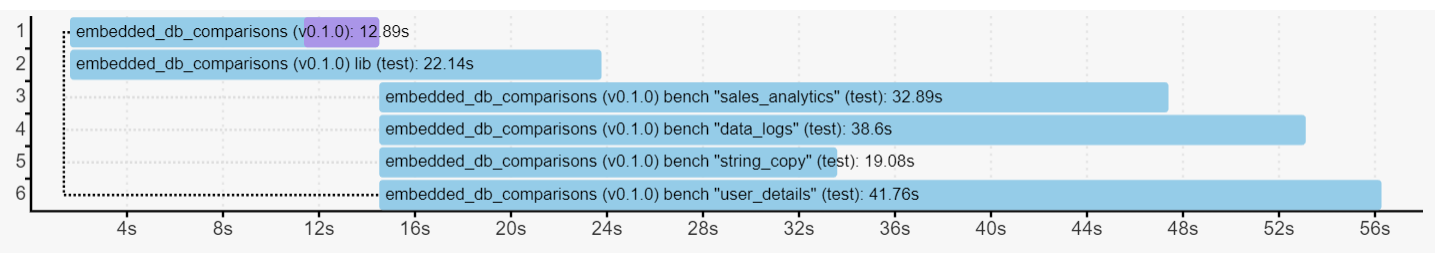
\includegraphics[width=\textwidth]{evaluation/images/recompile.png}
    \caption{Cargo timings for a recompile on no change of the embedded database comparison benchmarks.}
    \label{fig:recompile}
\end{figure}
\begin{figure}[h!]
    \centering
    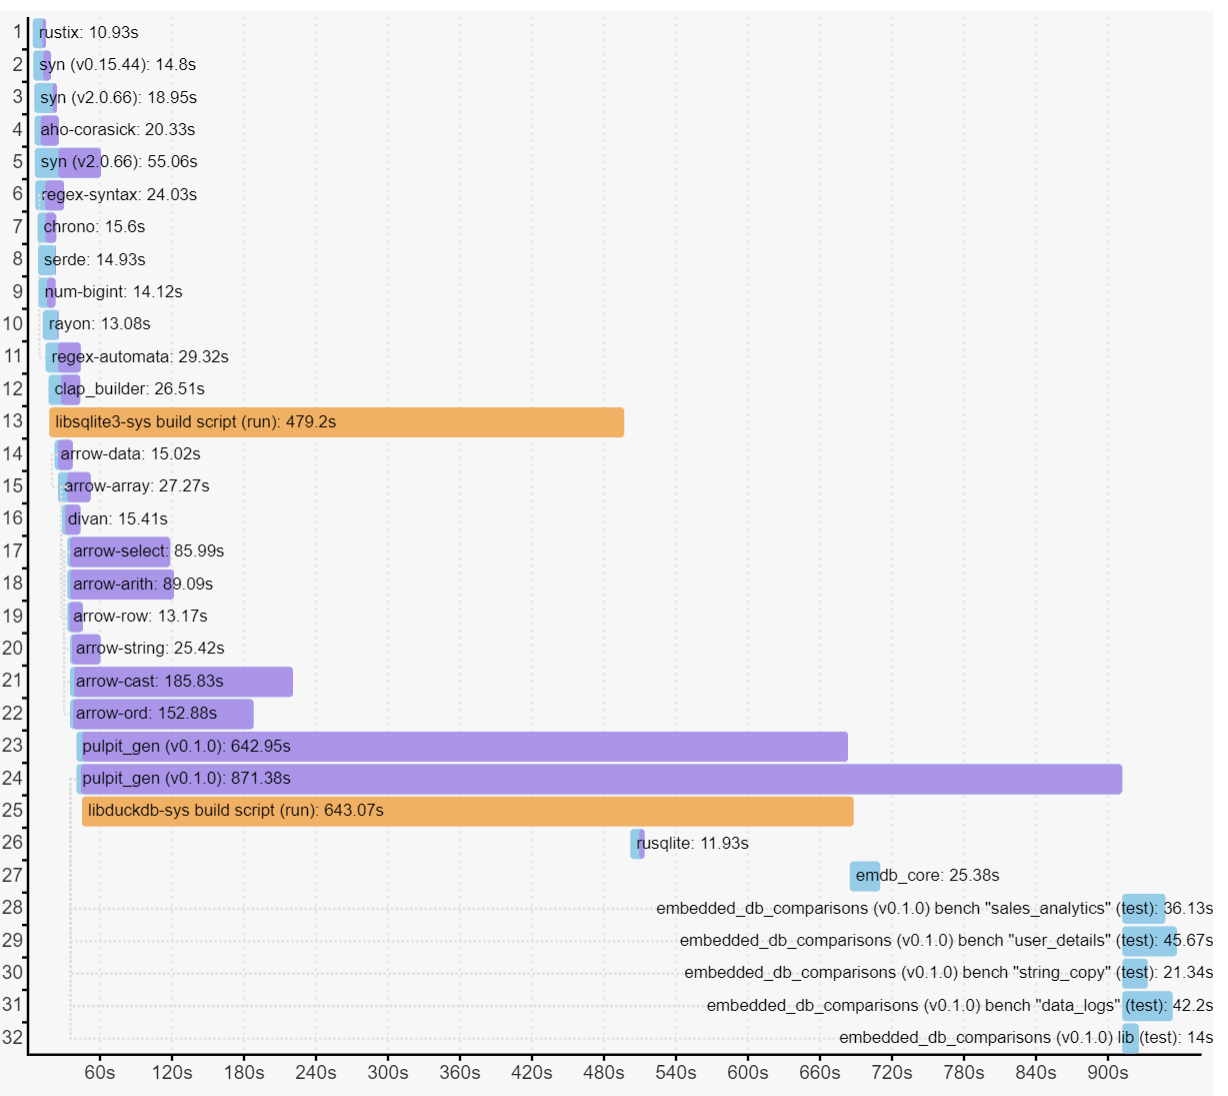
\includegraphics[width=\textwidth]{evaluation/images/fresh.png}
    \caption{Cargo timings for a fresh compilation of the embedded database comparison benchmarks.}
    \label{fig:freshcompile}
\end{figure}
\begin{itemize}
    \setlength\itemsep{0em}
    \item The initial compile takes significant time, however incremental builds afterward are fast enough for a responsive IDE experience.
    \item The cost of compiling DuckDB and SQLite is comparably large.
\end{itemize}
\begin{futurebox}{Feature gating crates}
    Improvements to the initial/from fresh compile time can be gained by feature gating unused features included in the emDB crate.
    \begin{itemize}
        \item Pulpit table generation macros are included in the emDB crate, for convenience, but are not a requirement to use the emQL macro.
    \end{itemize}
\end{futurebox}
\newpage
\begin{futurebox}{Improved trait resolution}
    Trait resolution\cite{TraitSolving} is an expensive operation. The heavy reliance on traits to define parameters for Combi combinators 
    is therefore a considerable cost to the initial/from fresh compile of emDB.
    \\
    \\ Combi is in fact so expensive, that some constructs cannot be compiled by the latest nightly or stable compilers (as of \mintinline{bash}{rustc 1.80.0-nightly (032af18af 2024-06-02)}).
    \\ (from \github{https://github.com/OliverKillane/emDB/blob/main/crates/pulpit_gen/src/macros/new_simple.rs}{emDB/pulpit\_gen/src/macros/new\_simple}).
    \begin{minted}{rust}
        mapall( MustField::new("name", getident),
        ( DefaultField::new("transactions", on_off, ||false),
          ( DefaultField::new("deletions", on_off, ||false),
            ( /* ... singificant nesting of Fields which construct a combinator tree ... */ )
         )
       )
    ).gen(':'),
    \end{minted}
    This will hopefully be improved through both performance improvements to rustc and in future the a Chalk-based trait solver.\cite{ChalktraitSolver}
\end{futurebox}

\section{[Qualitative] Ease of Use}
\begin{minted}{toml}
# in rust project `Cargo.toml`
[dependencies]
emdb = { git = "https://github.com/OliverKillane/emDB.git" }
\end{minted}
emDB generates rust diagnostics, which are already integrated with rust supporting IDEs.
This is not possible with either SQLite or DuckDB without using a tool like sqlx.
\begin{itemize}
    \setlength\itemsep{0em}
    \item The sqlx project contains several database access libraries, including the
          \mintinline{rust}{sqlx::query!} macro, which connects to a live database to syntax
          \& semantics check the queries.
    \item This requires the developer to keep a development database running for access. But also
          allows sqlx to work with a variety of different databases \& SQL variants.
    \item sqlx cannot propagate errors back to individual spans inside a query string.
\end{itemize}
\begin{figure}[h]
    \centering
    \includegraphics[width=\textwidth]{evaluation/_diagrams/compile_stages.pdf}
    \caption{Stages of error message generation}
    \label{fig:error_message_gen}
\end{figure}
A significant weakness of emDB is that the correctness of user embedded code depends on the optimisations applied to data structures.
\begin{itemize}
    \setlength\itemsep{0em}
    \item Values versus references for items gotten from tables, only known after analyzing all queries and determining the data structure to use.
    \item Structure selection requires the full context, so no code is generated (and hence user code checked) if there are any emQL semantic or syntactic errors.
\end{itemize}
Multiple syntax errors is managed by the Combi library (a part of this project), which allows for multiple syntax errors without error AST nodes, keeping the semantic analysis code relatively simple.

\begin{futurebox}{Allow both syntax and semantic Errors}
    Some language features are independent.
    \begin{itemize}
        \setlength\itemsep{0em}
        \item The emql syntax and semantics of independent queries.
        \item Queries that do not use a given table are independent of syntax or semantic errors with the table.
    \end{itemize}
    By adding some error AST nodes, or alternatively hoisting some of the semantic analysis in to Combi reporting more errors could be facilitated.
\end{futurebox}

\begin{center}
    \begin{tabular}{l | l l l l }
        \textbf{feature}                                  & \textbf{emDB} & \textbf{DuckDB} & \textbf{SQLite} & \textbf{SQLite + sqlx} \\
        \hline
        \textbf{\mintinline{bash}{Cargo.toml} only setup} & Yes           & Yes             & Yes             & No                     \\
        \textbf{Compile Time Checks}                      & Yes           & No              & No              & Yes                    \\
        \textbf{Identifier Precise Errors}                & Yes           & No              & No              & No                     \\
    \end{tabular}
\end{center}

\begin{futurebox}{User Survey}
    The syntax \& semantics of emql have been chosen through an iterative \textit{dogfooding} process, and lacks a more general justification.
    \begin{itemize}
        \setlength\itemsep{0em}
        \item User feedback requires a stabilization of the emQL interface and a commitment to support the library long term.
    \end{itemize}
\end{futurebox}

\section{Conclusion}
This project has been successful in implementing a novel, usable \& performant kind of embedded database that has not previously existed.
There remain significant opportunities to improve performance, both through optimising the current operator and table implementation, 
and by improving logical optimisations (most importantly incremental view maintenance). This will be aided by the simple, modular \& easy 
to use design of the emDB compiler.
